%%%%%%%%%%%%%%%%%%%%%%%%%%%%%%%%%%%%%%%%%%%%%%%%%%%%%%%%%%%%%%%%%%%%%%
% Overleaf (WriteLaTeX) Example: Molecular Chemistry Presentation
%
% Source: http://www.overleaf.com
%
% In these slides we show how Overleaf can be used with standard
% chemistry packages to easily create professional presentations.
%
% Feel free to distribute this example, but please keep the referral
% to overleaf.com
%
%%%%%%%%%%%%%%%%%%%%%%%%%%%%%%%%%%%%%%%%%%%%%%%%%%%%%%%%%%%%%%%%%%%%%%

\documentclass[xcolor={dvipsnames}]{beamer}

\mode<presentation>
{
  \usetheme{Madrid}       % or try default, Darmstadt, Warsaw, ...
  \usecolortheme{default} % or try albatross, beaver, crane, ...
  \usefonttheme{default}    % or try default, structurebold, ...
  \setbeamertemplate{navigation symbols}{}
  \setbeamertemplate{caption}[numbered]
}

\usepackage[english]{babel}
\usepackage[utf8x]{inputenc}
\usepackage{graphicx}
\usepackage{hyperref}
  \hypersetup{colorlinks=true}
  \hypersetup{urlcolor=blue}
  \hypersetup{linkcolor = .}
\usepackage{xcolor}
\usepackage{siunitx}
  \sisetup{separate-uncertainty = true}
\DeclareSIUnit\barn{b}
\usepackage{physics}
\usepackage[font=small,labelfont=bf]{caption}
\usepackage{subcaption}
\usepackage[en-GB]{datetime2}
\usepackage{overpic}
\usepackage{feynmp}
\DeclareGraphicsRule{*}{mps}{*}{}
\usepackage{scalerel}
\newcommand{\mylbrace}[2]{\vspace{#2pt}\hspace{6pt}\scaleleftright[\dimexpr5pt+#1\dimexpr0.06pt]{\lbrace}{\rule[\dimexpr2pt-#1\dimexpr0.5pt]{-4pt}{#1pt}}{.}}
\newcommand{\myrbrace}[2]{\vspace{#2pt}\scaleleftright[\dimexpr5pt+#1\dimexpr0.06pt]{.}{\rule[\dimexpr2pt-#1\dimexpr0.5pt]{-4pt}{#1pt}}{\rbrace}\hspace{6pt}}

% Trim in percent
\usepackage{adjustbox}

% No "Figure" prefix
\setbeamertemplate{caption}{\raggedright\insertcaption\par}

% Nice decay amplitude diagrams
\usepackage{amsmath,amssymb,tikz-cd}

% Strike out text
\usepackage[normalem]{ulem}

% For figures with text overlay
\usepackage{overpic}

% Arrows
\usepackage{tikz}
\newcommand{\tikzmark}[1]{\tikz[remember picture] \node[coordinate] (#1) {#1};}

% Colourbox with line breaks
\newcommand{\cbox}[2][lime!20]{%
  \colorbox{#1}{\parbox{\dimexpr\linewidth-2\fboxsep}{\strut #2\strut}}%
}

% Vector arrows
\usepackage[pdftex]{pict2e}

% Checkmark symbol
\def\checkmark{\tikz\fill[scale=0.4](0,.35) -- (.25,0) -- (1,.7) -- (.25,.15) -- cycle;}

% Here's where the presentation starts, with the info for the title slide
\title[RTA WP2 meeting]{Update on forward tracking parameterisation update}

\author[Martin Tat]{Martin Tat}
\institute[Heidelberg]{Heidelberg University}
\date{10th June 2025}

\titlegraphic{
\includegraphics[height = 2.3cm]{lhcb.jpg}\hspace{1.0cm}~%
              
\includegraphics[height = 2.3cm]{HeidelbergLogo.pdf}}

\begin{document}

\begin{frame}
  \titlepage
\end{frame}

% These three lines create an automatically generated table of contents.
\begin{frame}{Outline}
  \tableofcontents
\end{frame}

\section{Introduction and reminder of previous presentation}

\begin{frame}{Introduction}
  \vspace{0.0cm}
  {\Large I previously presented an update on the HLT2 forward tracking parameterisations}
  \vspace{0.5cm}
  \begin{itemize}
    \setlength\itemsep{1.0em}
    \item{\href{https://indico.cern.ch/event/1541826/\#13-update-of-pattern-recogniti}{Link to Indico here}}
    \item{Tracking algorithm described in three steps:}
    \begin{enumerate}
      \item{Trajectories based on equations of motion and detector geometry}
      \item{Parameterise complex calculations using polynomials}
      \item{Determine coefficients by fits to MC}
    \end{enumerate}
    \item{Parameterisations updated using new MC samples}
    \begin{itemize}
      \item{New magnetic field map (presented \href{https://indico.cern.ch/event/1539235/\#3-update-magnetic-field-map}{here})}
      \item{Initially worked with a private MC production}
      \item{Moved to centrally produced samples \href{https://gitlab.cern.ch/lhcb-simulation/mc-requests/-/merge_requests/1208}{here}}
    \end{itemize}
  \end{itemize}
\end{frame}

\begin{frame}{Reminder: Parameterisations in HLT2 forward tracking}
  \vspace{0.0cm}
  {\large Last time I presented these parameterisations:}
  \vspace{0.2cm}
  \begin{enumerate}
    \setlength\itemsep{0.5em}
    \item{$z$ magnet kick position}
    \item{$x$ fringe field correction}
    \item{Stereo angle $y$ correction}
    \item{Hough histogram binning}
    \item{$z$ hit correction with SciFi $yz$ tilt}
    \item{Magnetic field integral}
  \end{enumerate}
\end{frame}

\begin{frame}{Reminder: Parameterisations in HLT2 forward tracking}
  \vspace{0.0cm}
  {\large Last time I presented these parameterisations:}
  \vspace{0.2cm}
  \begin{enumerate}
    \setlength\itemsep{0.5em}
    \item{$z$ magnet kick position $\leftarrow$ Caused some issues}
    \item{$x$ fringe field correction}
    \item{Stereo angle $y$ correction}
    \item{Hough histogram binning}
    \item{$z$ hit correction with SciFi $yz$ tilt}
    \item{Magnetic field integral}
  \end{enumerate}
\end{frame}

\begin{frame}{Reminder: Parameterisations in HLT2 forward tracking}
  \vspace{0.0cm}
  {\large Last time I presented these parameterisations:}
  \vspace{0.2cm}
  \begin{enumerate}
    \setlength\itemsep{0.5em}
    \item{$z$ magnet kick position}
    \item{$x$ fringe field correction}
    \item{Stereo angle $y$ correction}
    \item{Hough histogram binning}
    \item{$z$ hit correction with SciFi $yz$ tilt}
    \item{Magnetic field integral $\leftarrow$ Improves momentum resolution estimate}
  \end{enumerate}
\end{frame}

\begin{frame}{Reminder: $z_{\rm mag}$ parameterisation}
  \vspace{0.0cm}
  \begin{figure}[htb]
    \centering
    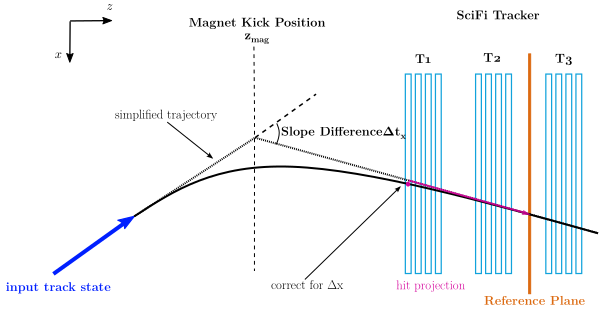
\includegraphics[width=0.75\textwidth]{Plots/MagnetKinkPosition.png}
    \caption*{\small From CERN-THESIS-2023-097}
  \end{figure}
  \begin{itemize}
    \item{Simplified track model: Assume magnet ``kicks'' particle at $z = z_{\rm mag}$}
    \item{Parameterise $z_{\rm mag}$ as:}
  \end{itemize}
  \begin{equation*}
    z_{\rm mag} = c_0 + c_1t_x^2 + c_3t_y^2 + \Delta t_x^\prime(c_2t_x + c_4\Delta t_x^\prime)
  \end{equation*}
\end{frame}

\begin{frame}{Reminder: Hit mapping to reference plane}
  \vspace{0.0cm}
  \begin{figure}[htb]
    \centering
    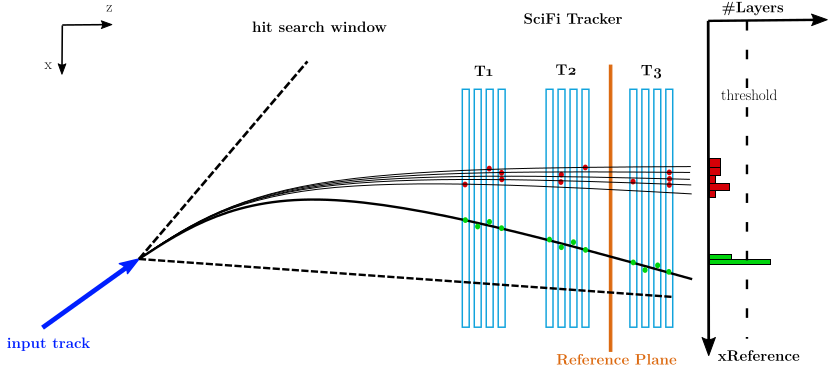
\includegraphics[width=1\textwidth]{Plots/HoughTransform.png}
  \caption*{\small From CERN-THESIS-2023-097}
  \end{figure}
  \vspace{-0.3cm}
  \begin{itemize}
    \item{Once all SciFi hits are parameterised, map hits to reference plane}
    \item{Hits from real tracks show peaks in ``Hough histogram''}
  \end{itemize}
\end{frame}

\begin{frame}{Reminder: Hit mapping to reference plane}
  \vspace{0.0cm}
  \begin{figure}[htb]
    \centering
    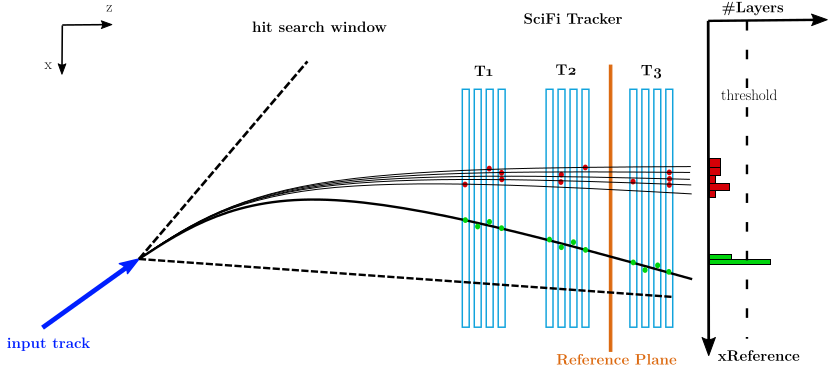
\includegraphics[width=1\textwidth]{Plots/HoughTransform.png}
  \caption*{\small From CERN-THESIS-2023-097}
  \end{figure}
  \vspace{-0.3cm}
  \begin{itemize}
    \item{Mapping depends on momentum, as low momentum tracks bend more}
    \item{Define a search window by assuming $p = p_{\rm min} = 1500$~MeV/c}
  \end{itemize}
\end{frame}

\begin{frame}{Reminder: Tracking efficiencies with new parameterisation}
  \vspace{0.0cm}
  {\Large Previously: Performance found to be worse after update}
  \vspace{0.5cm}
  \begin{itemize}
    \setlength\itemsep{1.0em}
    \item{Traced back to the $z_{\rm mag}$ parameterisation}
    \item{Reverting back to old $z_{\rm mag}$ parameterisation}
    \begin{itemize}
      \item[-]{Negligible change in performance compared to \texttt{2025-patches}}
    \end{itemize}
    \item{Possible explanation: Biases in $z_{\rm mag}$ are larger with new MC}
  \end{itemize}
\end{frame}

\begin{frame}{Reminder: Tracking efficiencies with new parameterisation}
  \vspace{0.0cm}
  \begin{figure}[htb]
    \centering
    \begin{subfigure}{0.45\textwidth}
      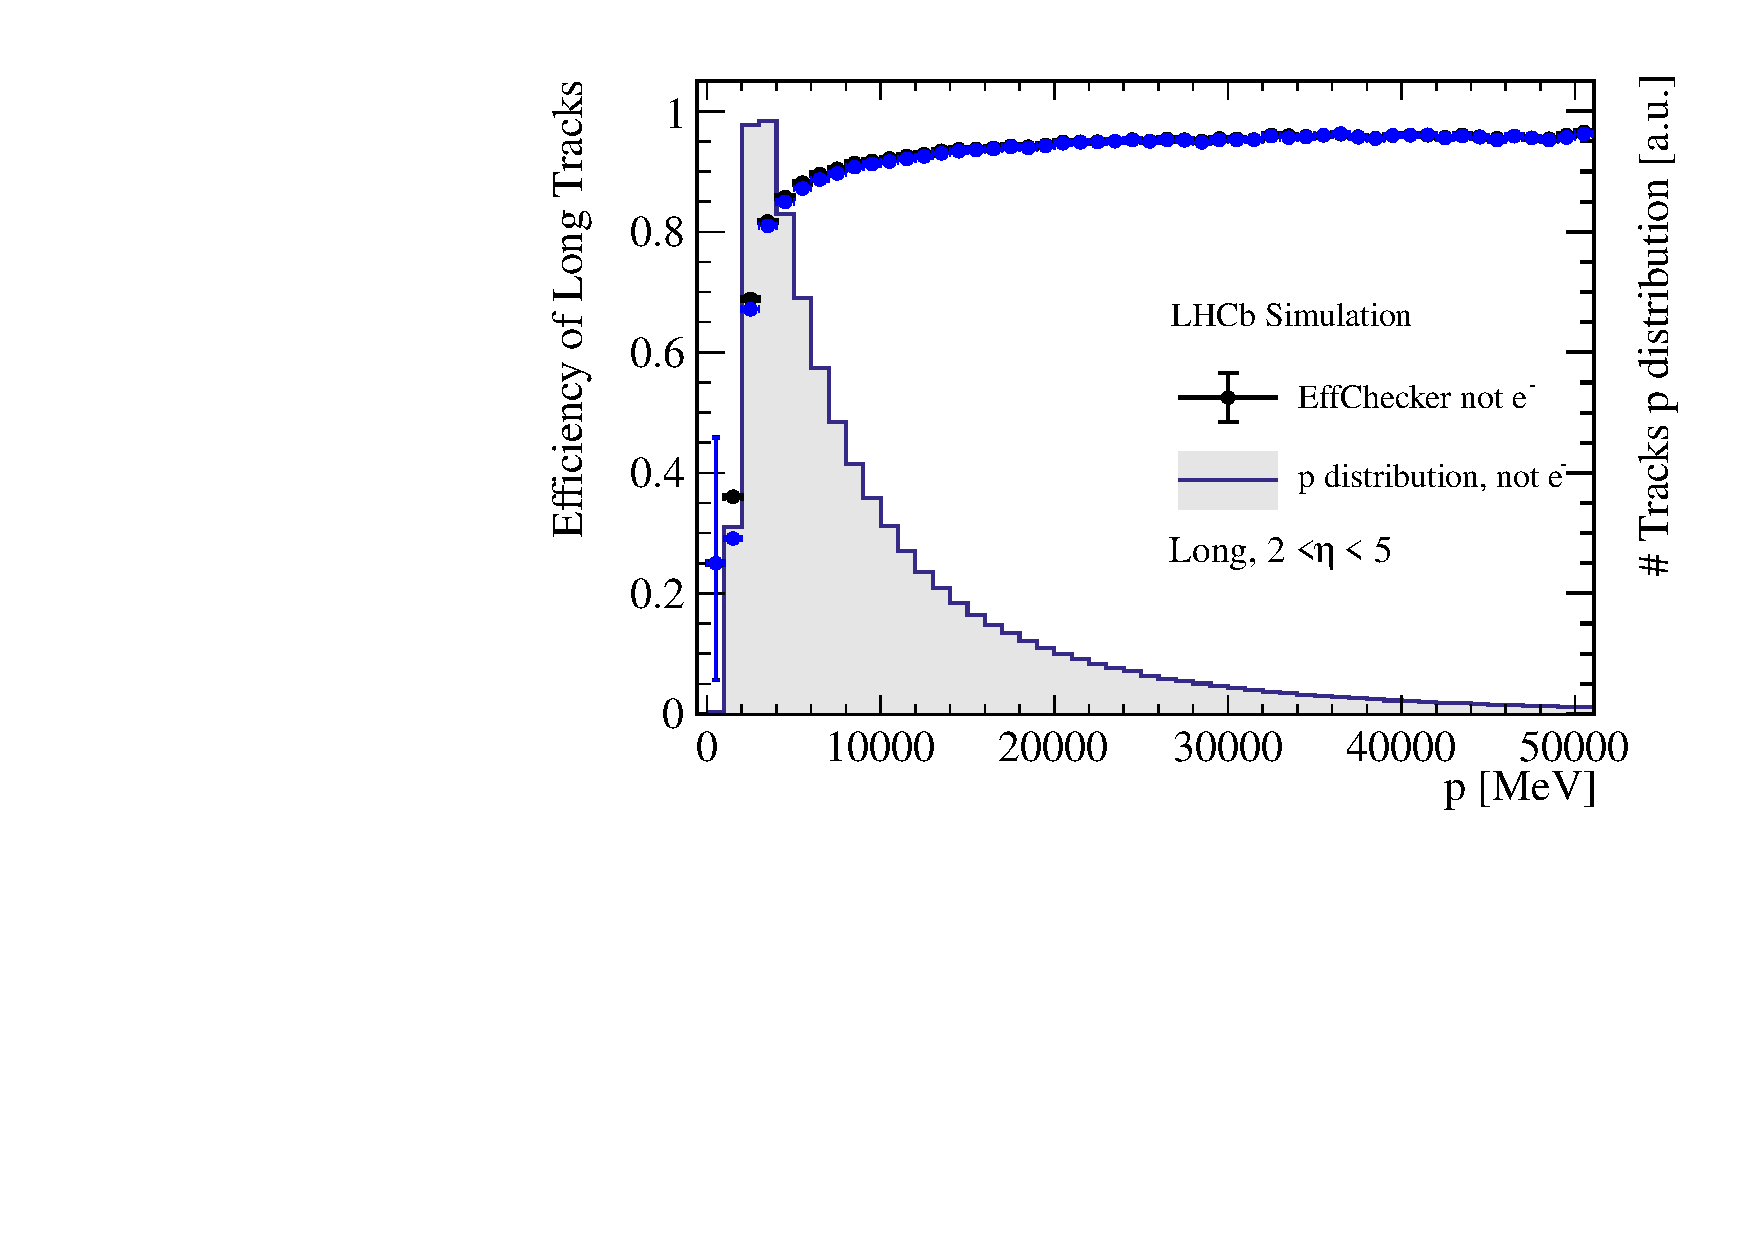
\includegraphics[width=1\textwidth]{Plots/TrackEfficiency_p_bad_MC_parameterisation.pdf}
    \end{subfigure}%
    \begin{subfigure}{0.45\textwidth}
      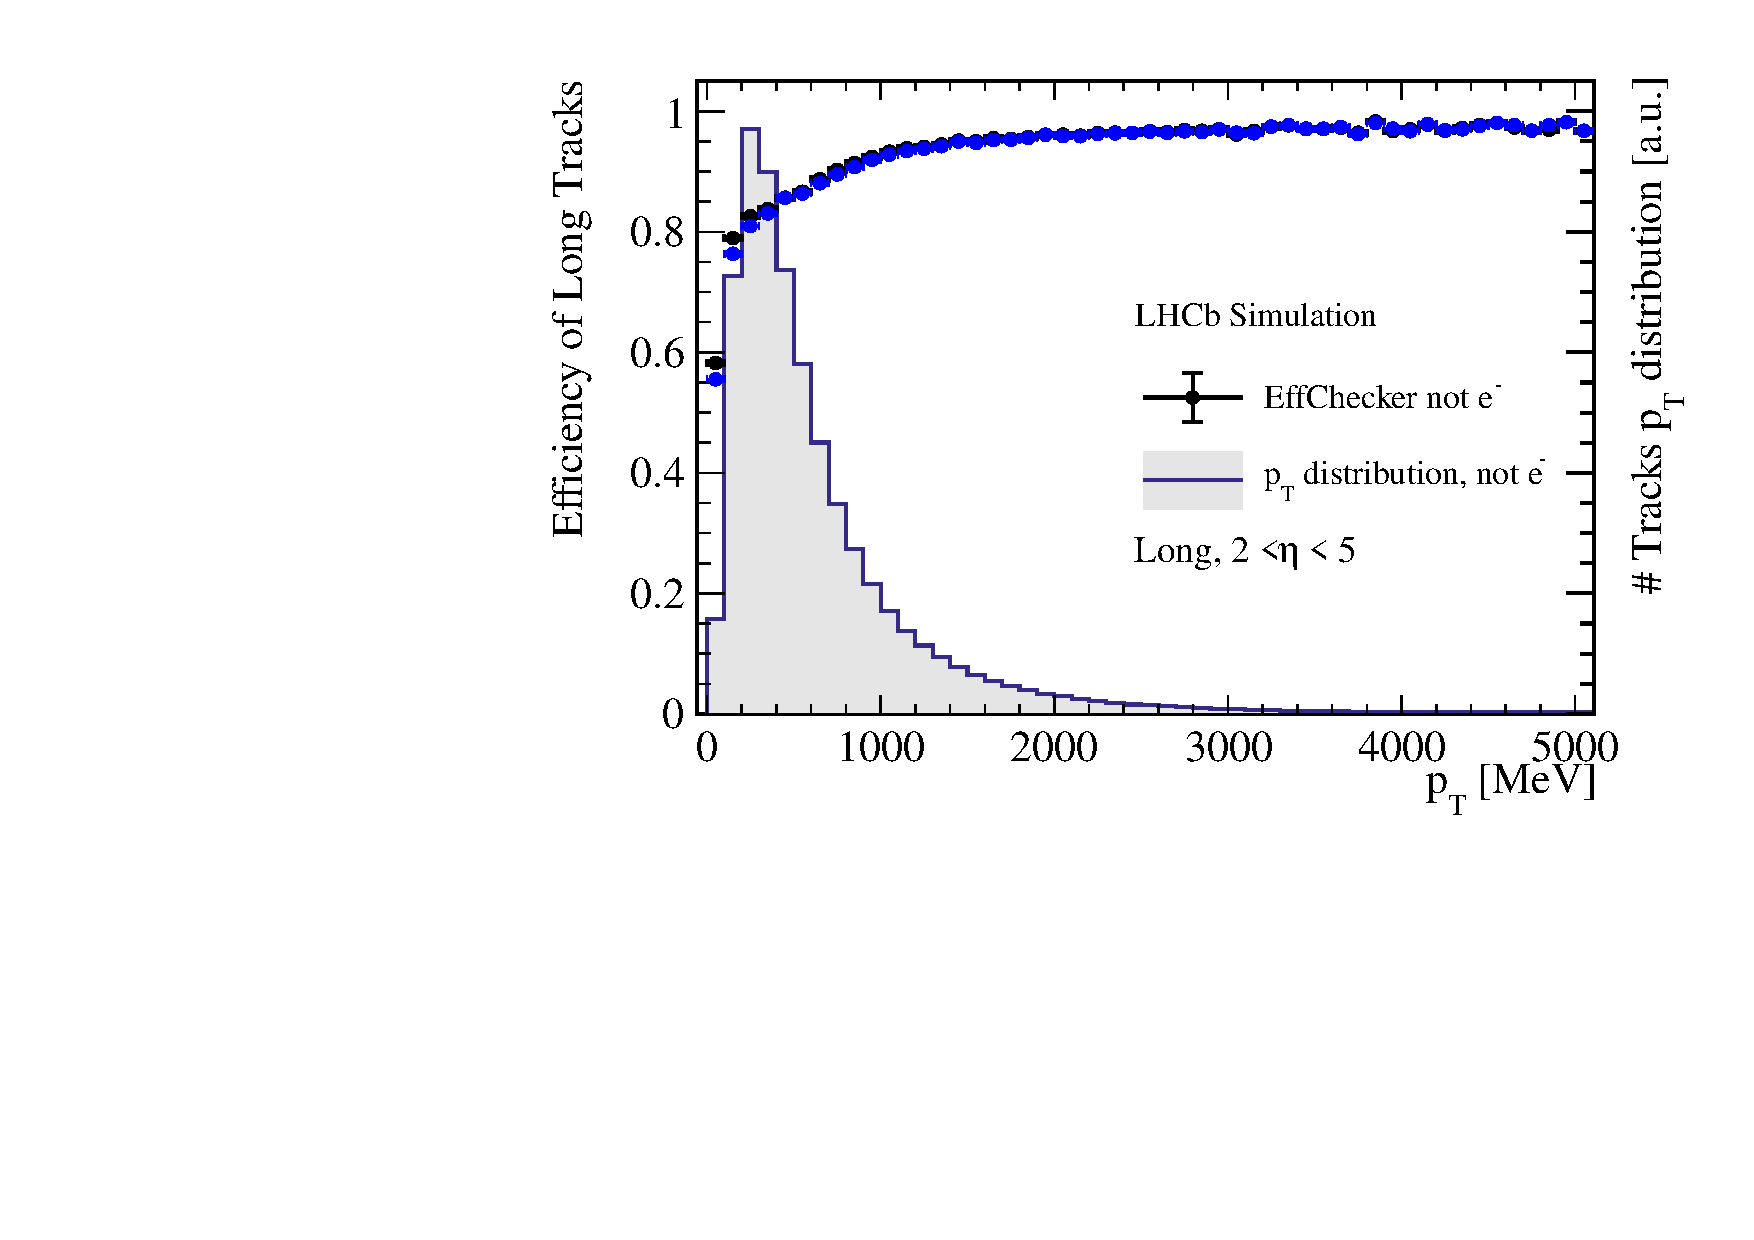
\includegraphics[width=1\textwidth]{Plots/TrackEfficiency_pt_bad_MC_parameterisation.pdf}
    \end{subfigure}
    \begin{subfigure}{0.45\textwidth}
      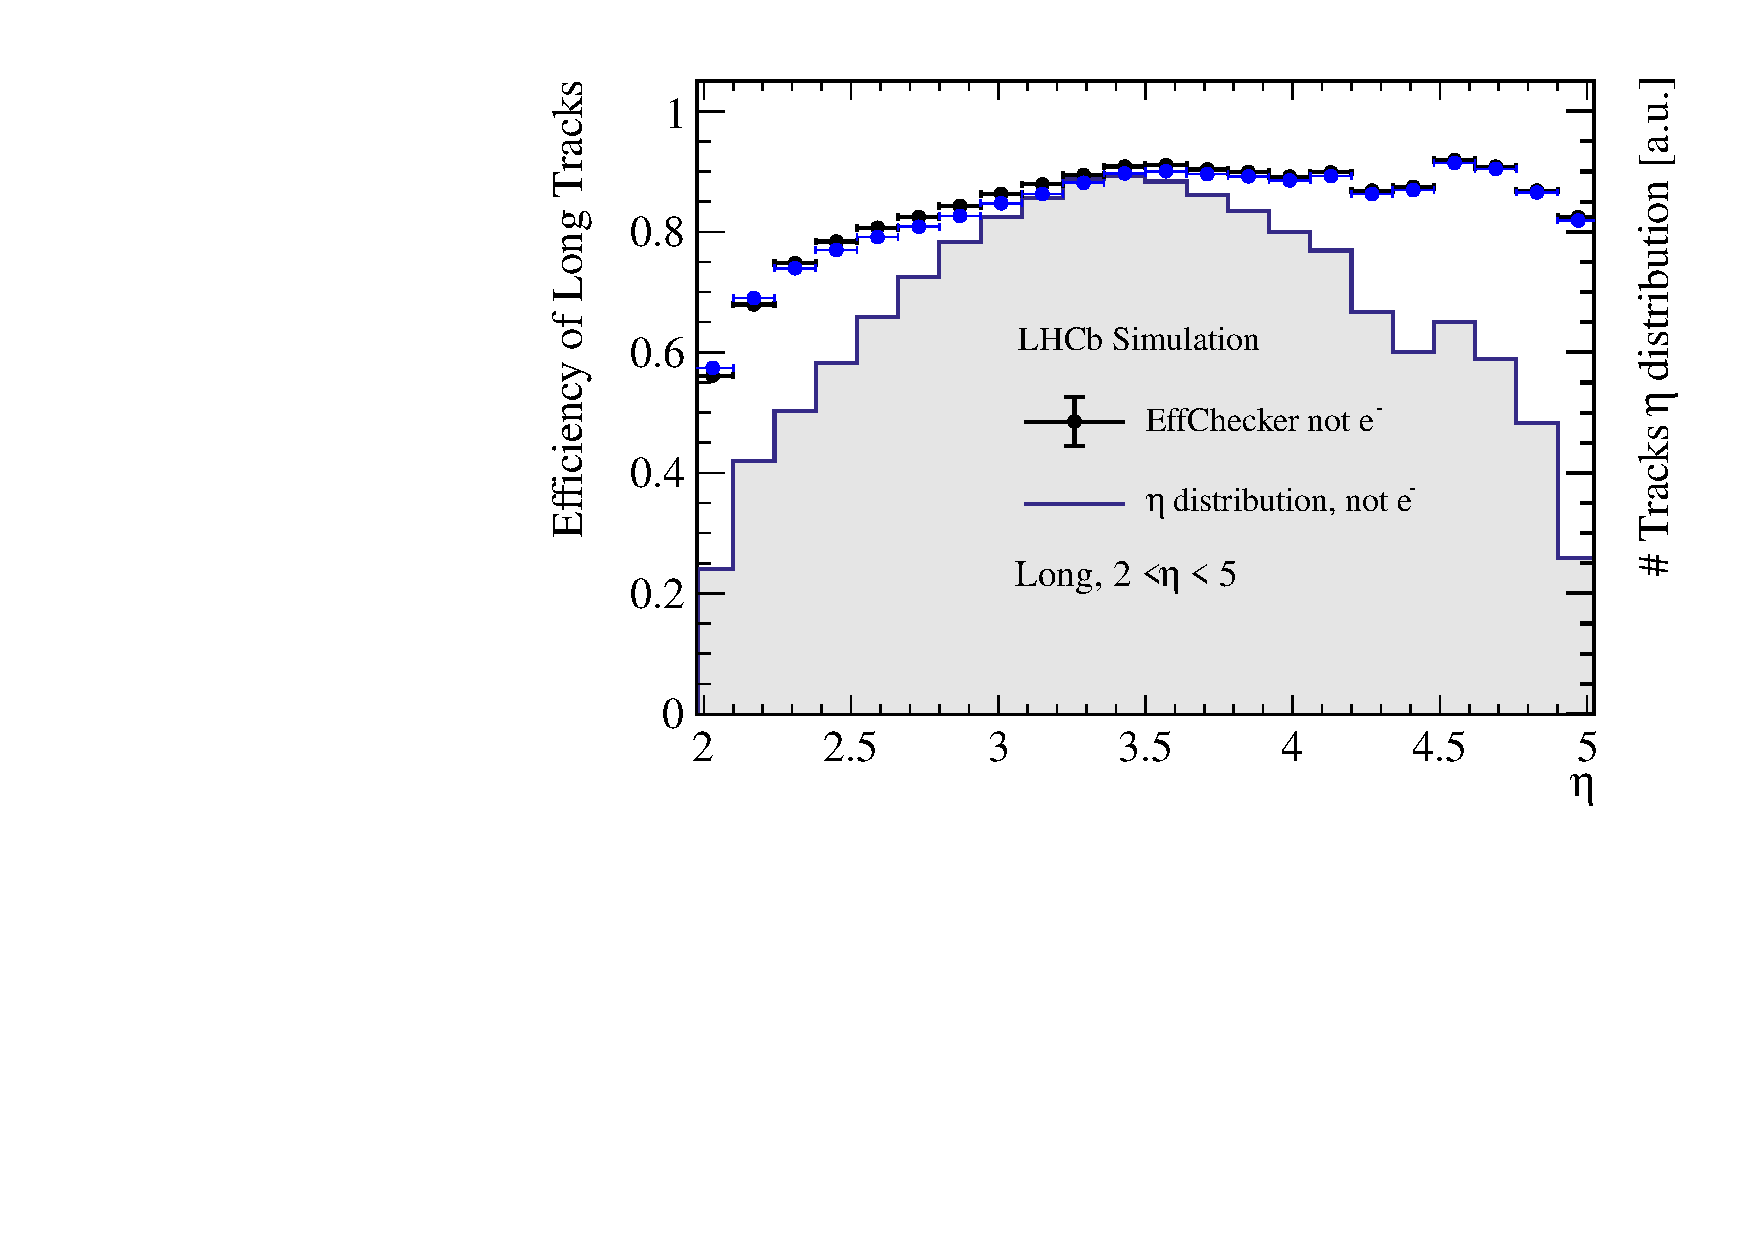
\includegraphics[width=1\textwidth]{Plots/TrackEfficiency_eta_bad_MC_parameterisation.pdf}
    \end{subfigure}%
    \begin{subfigure}{0.45\textwidth}
      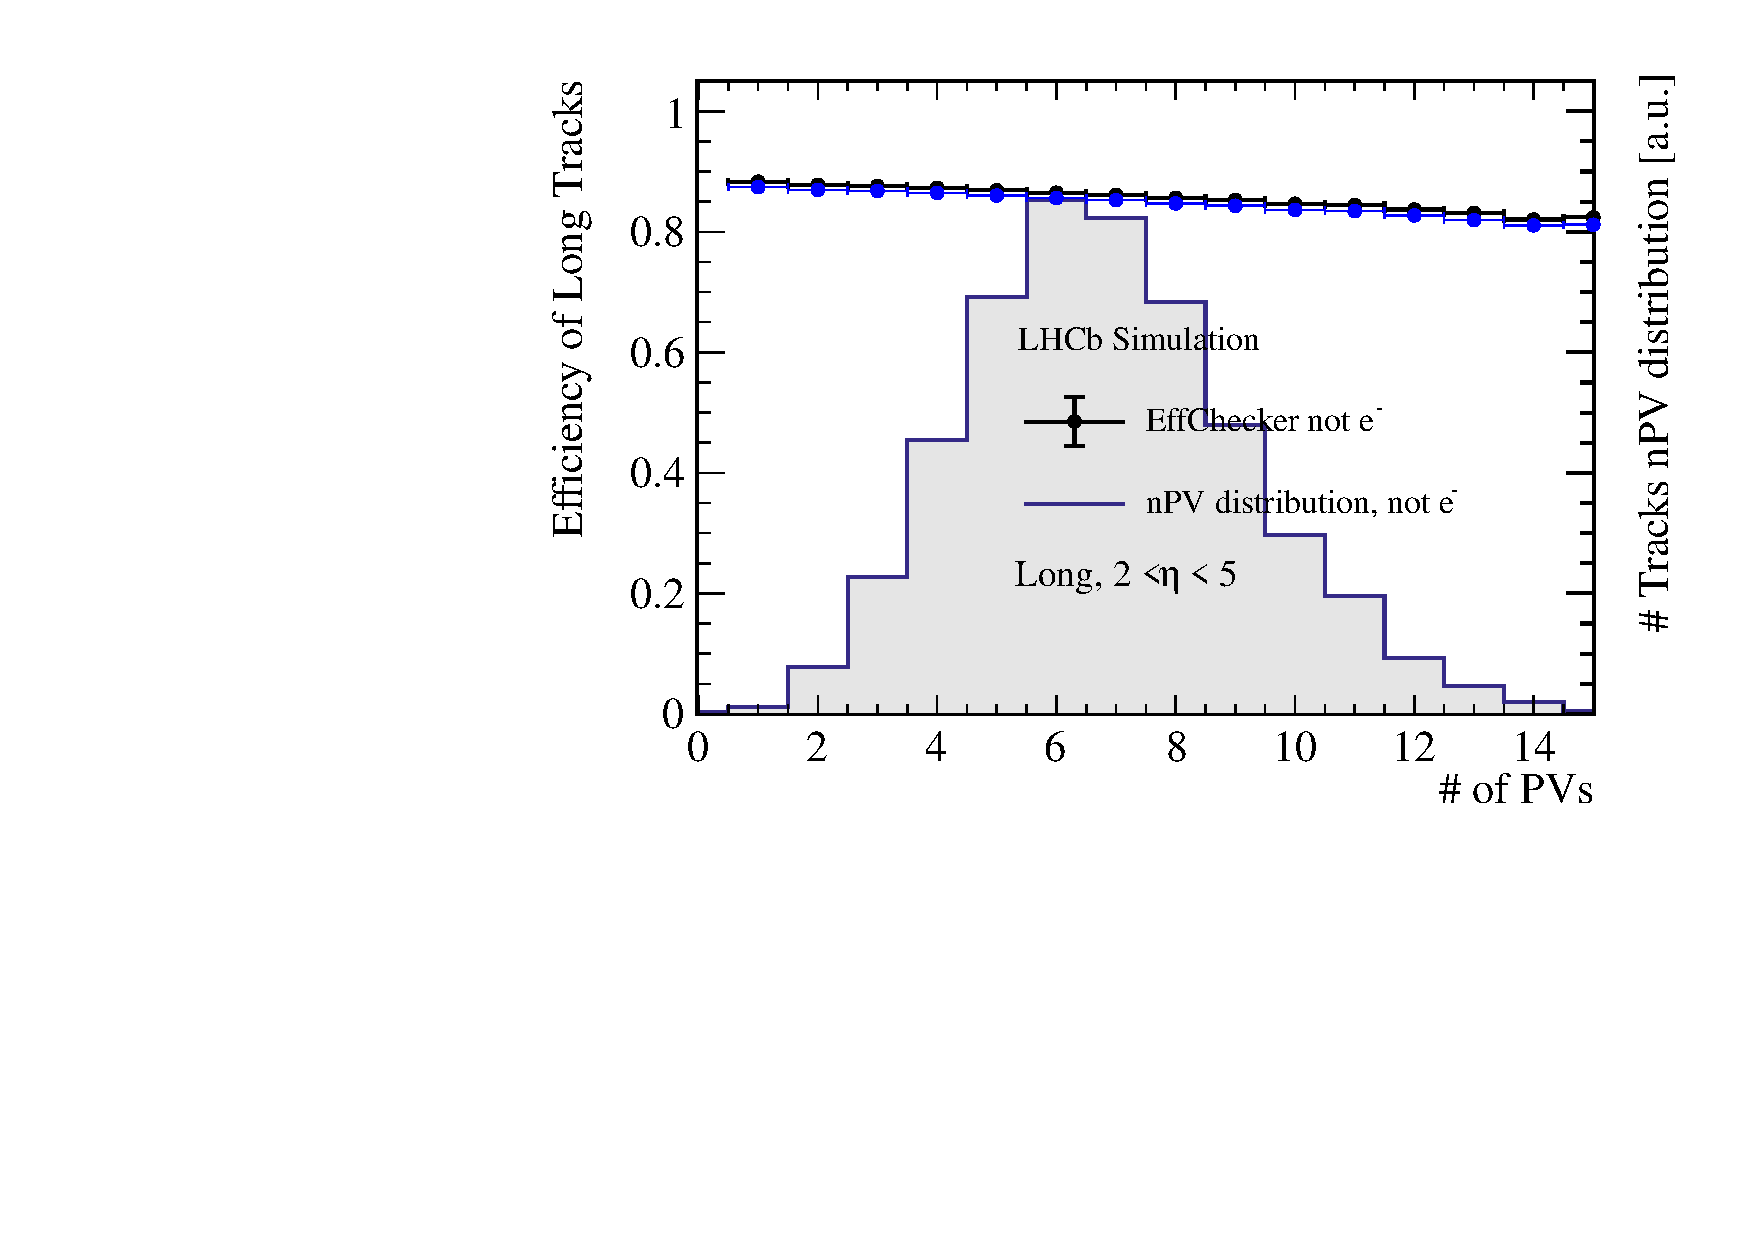
\includegraphics[width=1\textwidth]{Plots/TrackEfficiency_nPV_bad_MC_parameterisation.pdf}
    \end{subfigure}
    \vspace{-0.2cm}
    \caption*{Black: Old parameterisation. {\color{blue}Blue: Updated parameterisation}.}
  \end{figure}
\end{frame}

\begin{frame}{Reminder: Tracking efficiencies with new parameterisation}
  \vspace{0.0cm}
  \begin{figure}[htb]
    \centering
    \begin{subfigure}{0.45\textwidth}
      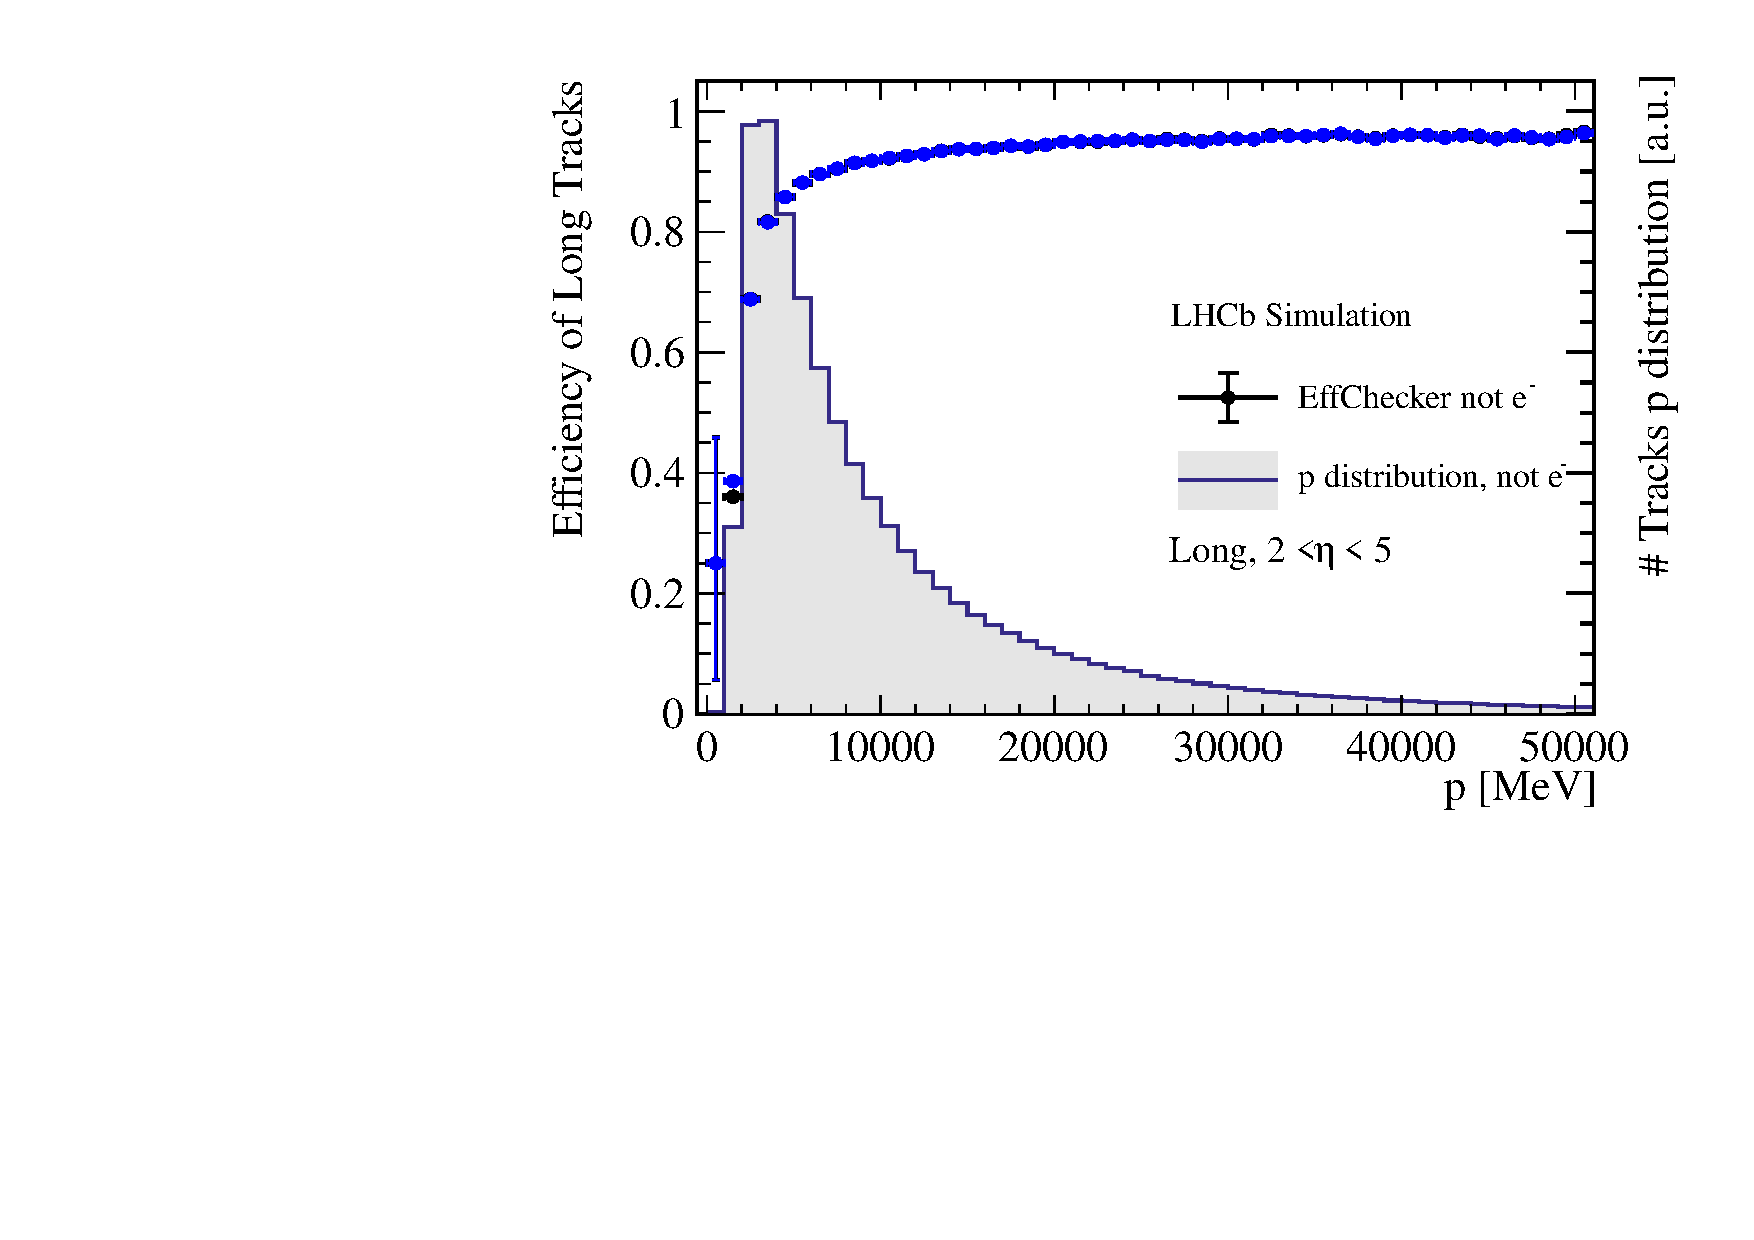
\includegraphics[width=1\textwidth]{Plots/TrackEfficiency_p_improved_MC_parameterisation.pdf}
    \end{subfigure}%
    \begin{subfigure}{0.45\textwidth}
      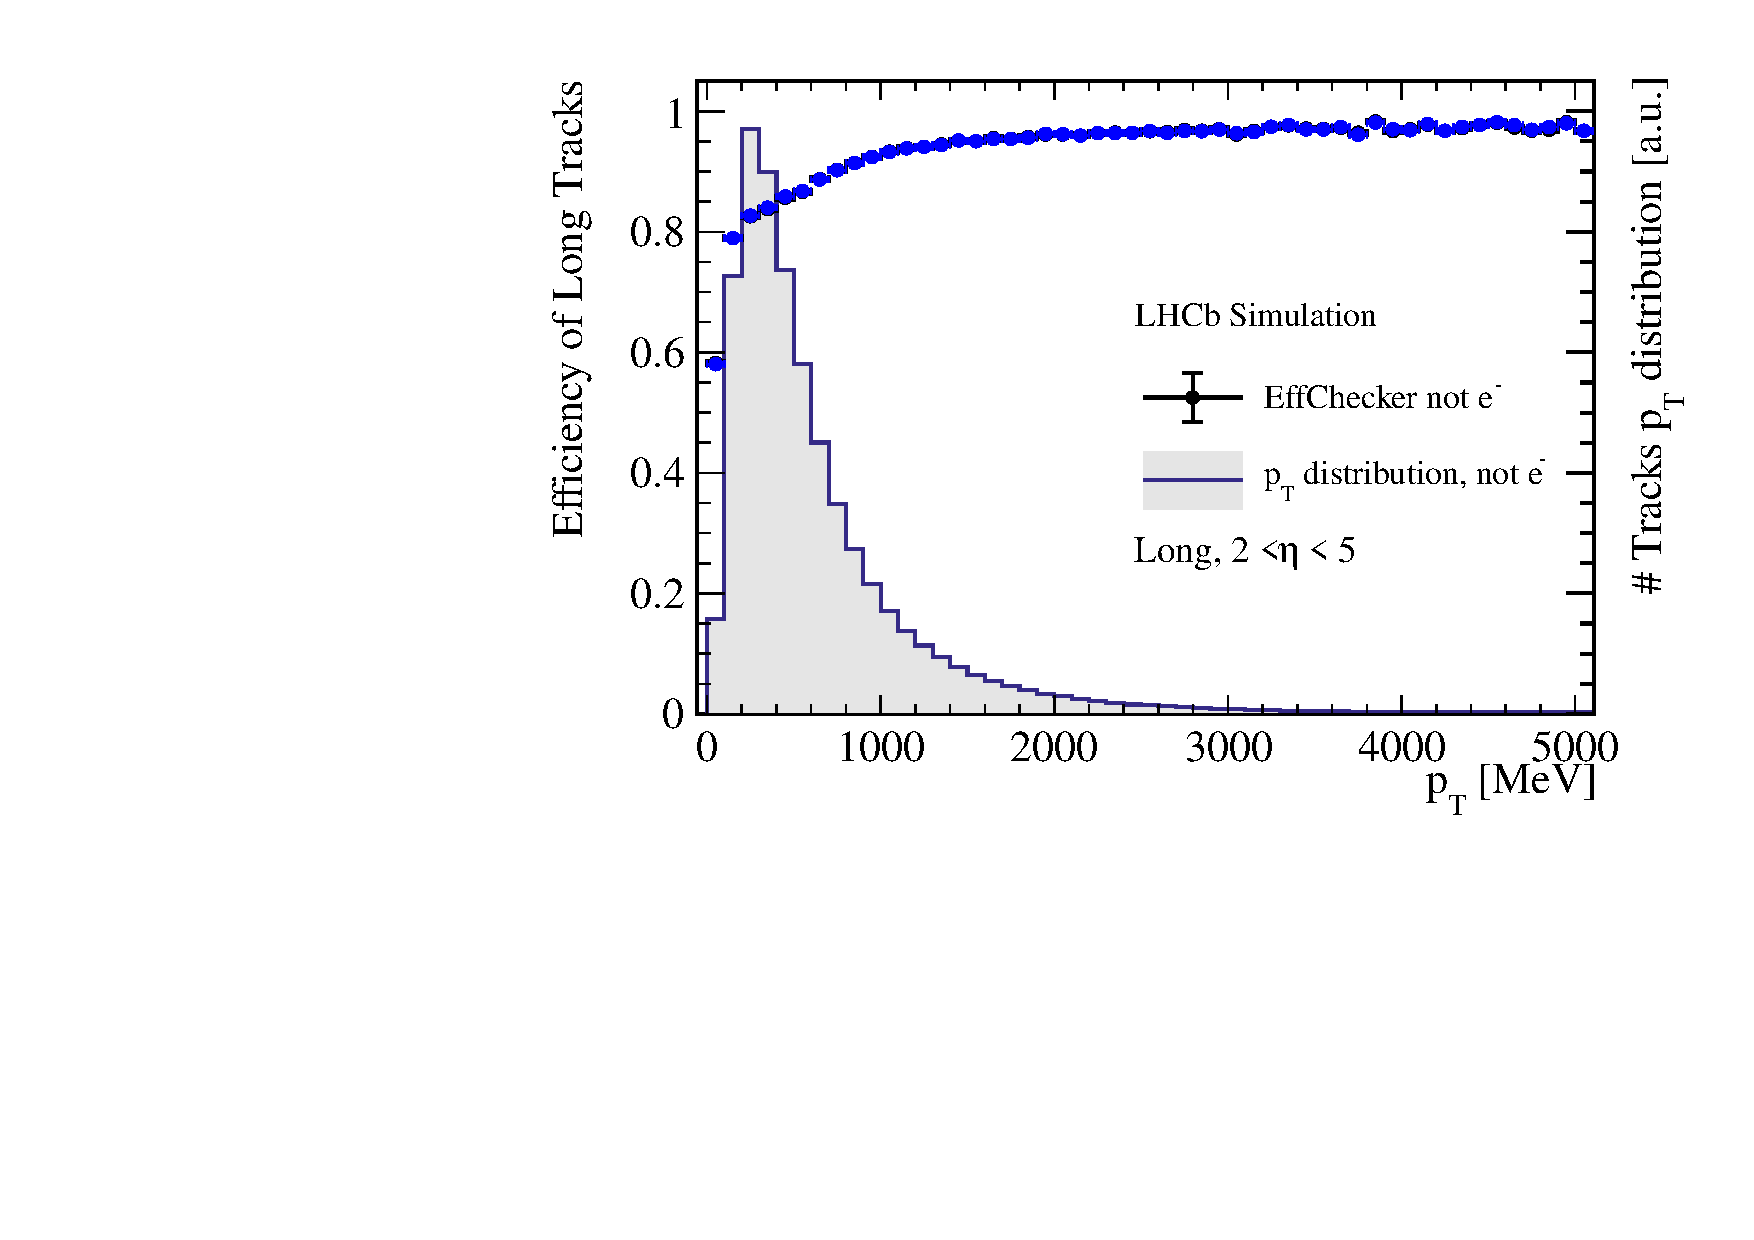
\includegraphics[width=1\textwidth]{Plots/TrackEfficiency_pt_improved_MC_parameterisation.pdf}
    \end{subfigure}
    \begin{subfigure}{0.45\textwidth}
      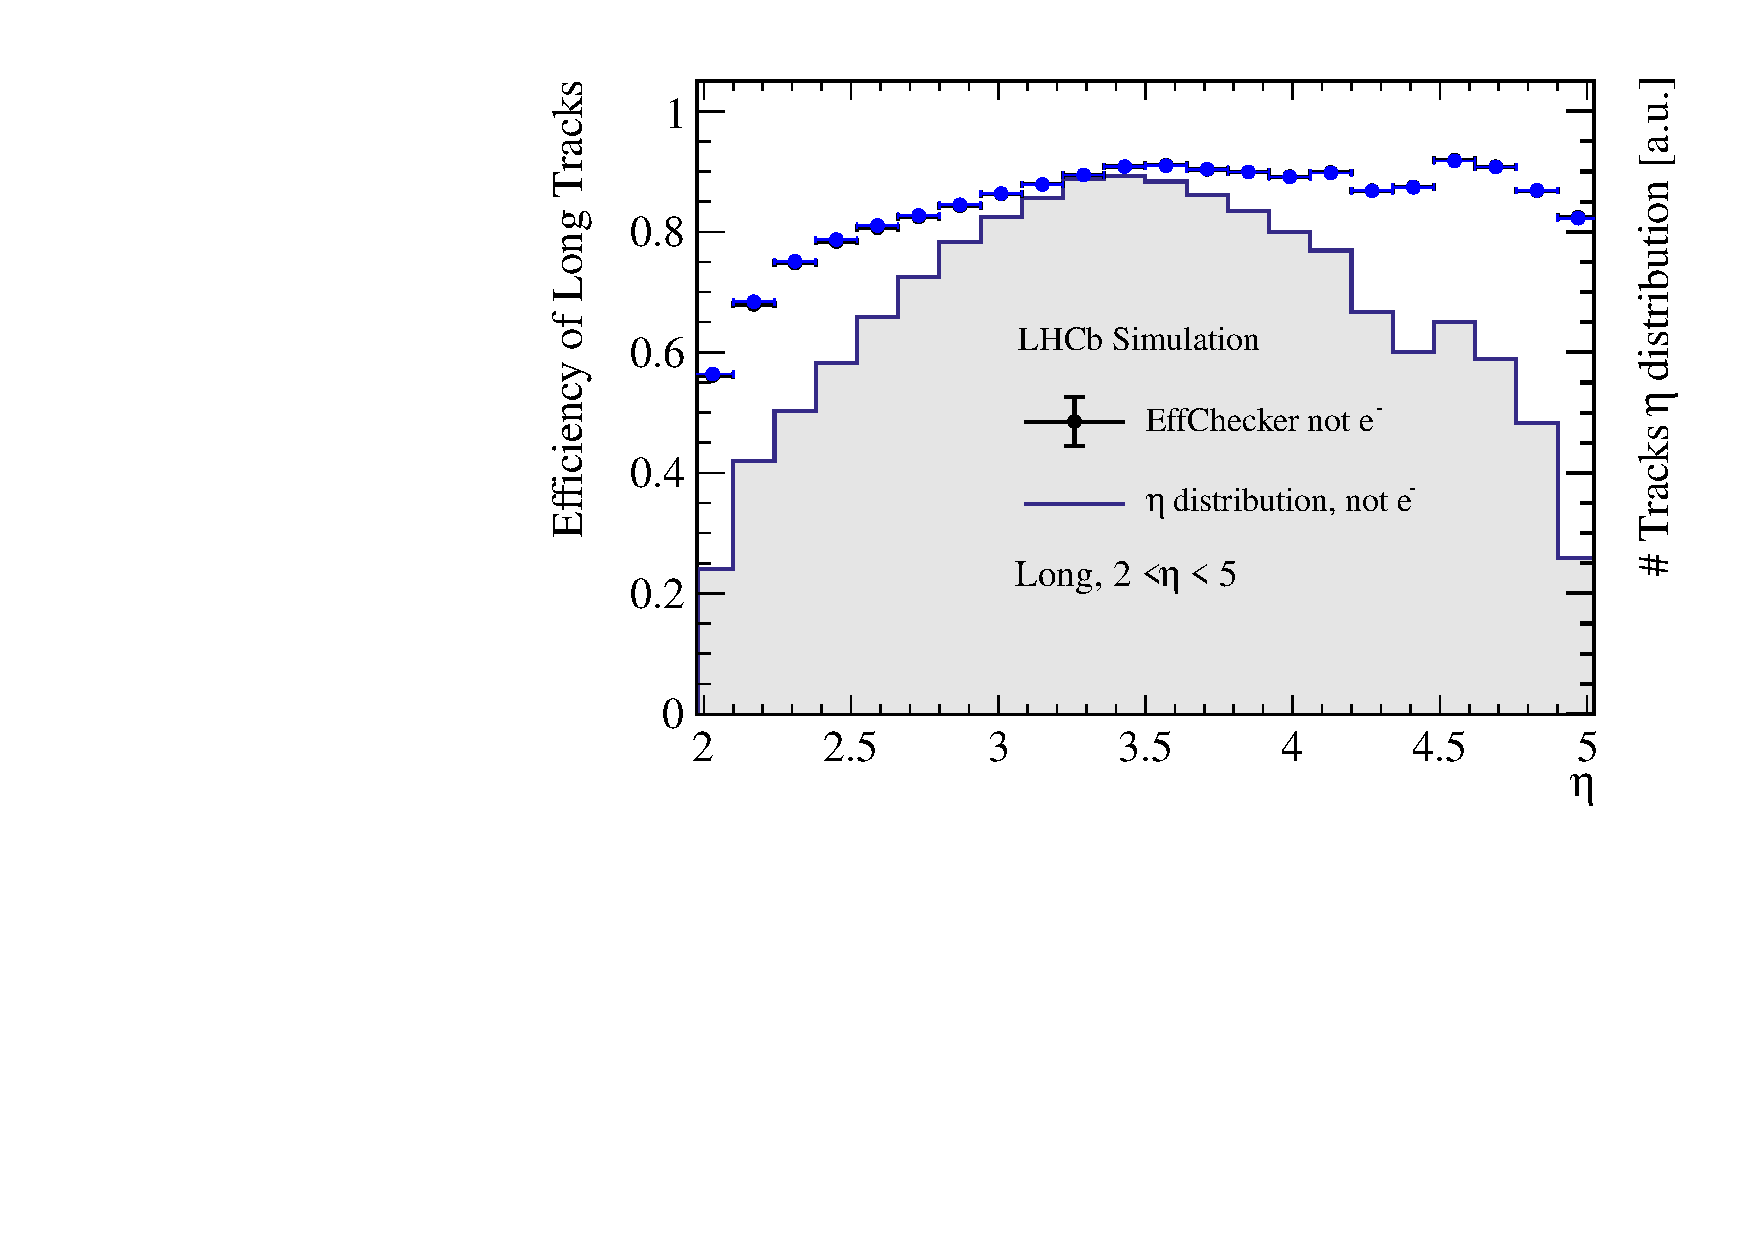
\includegraphics[width=1\textwidth]{Plots/TrackEfficiency_eta_improved_MC_parameterisation.pdf}
    \end{subfigure}%
    \begin{subfigure}{0.45\textwidth}
      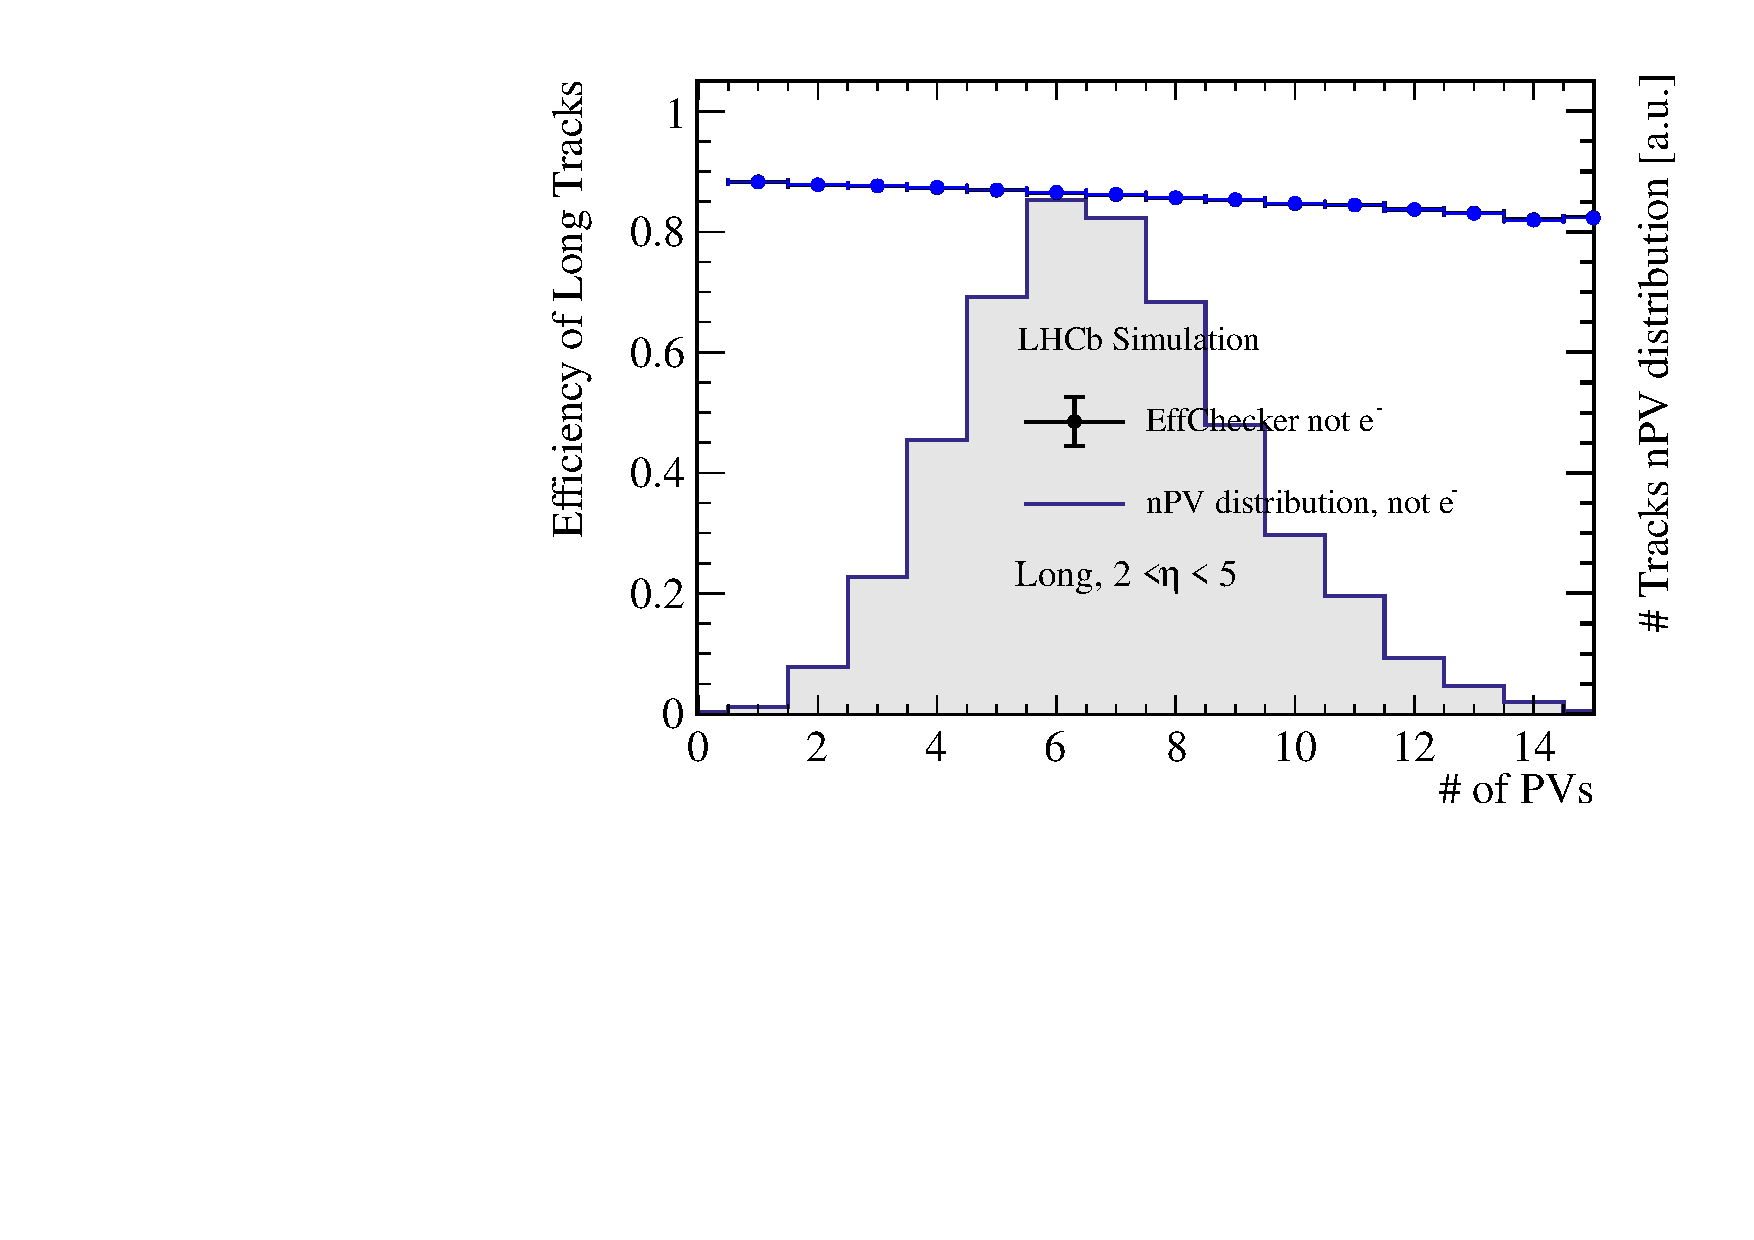
\includegraphics[width=1\textwidth]{Plots/TrackEfficiency_nPV_improved_MC_parameterisation.pdf}
    \end{subfigure}
    \vspace{-0.2cm}
    \caption*{Black: Old parameterisation. {\color{blue}Blue: Updated parameterisation with old $z_{\rm mag}$}.}
  \end{figure}
\end{frame}

\begin{frame}{Reminder: Momentum resolution}
  \vspace{0.0cm}
  {\Large Despite difficulties with $z_{\rm mag}$, it would be ideal to update parameterisations using the new field map}
  \begin{figure}[htb]
    \centering
    \begin{subfigure}{0.50\textwidth}
      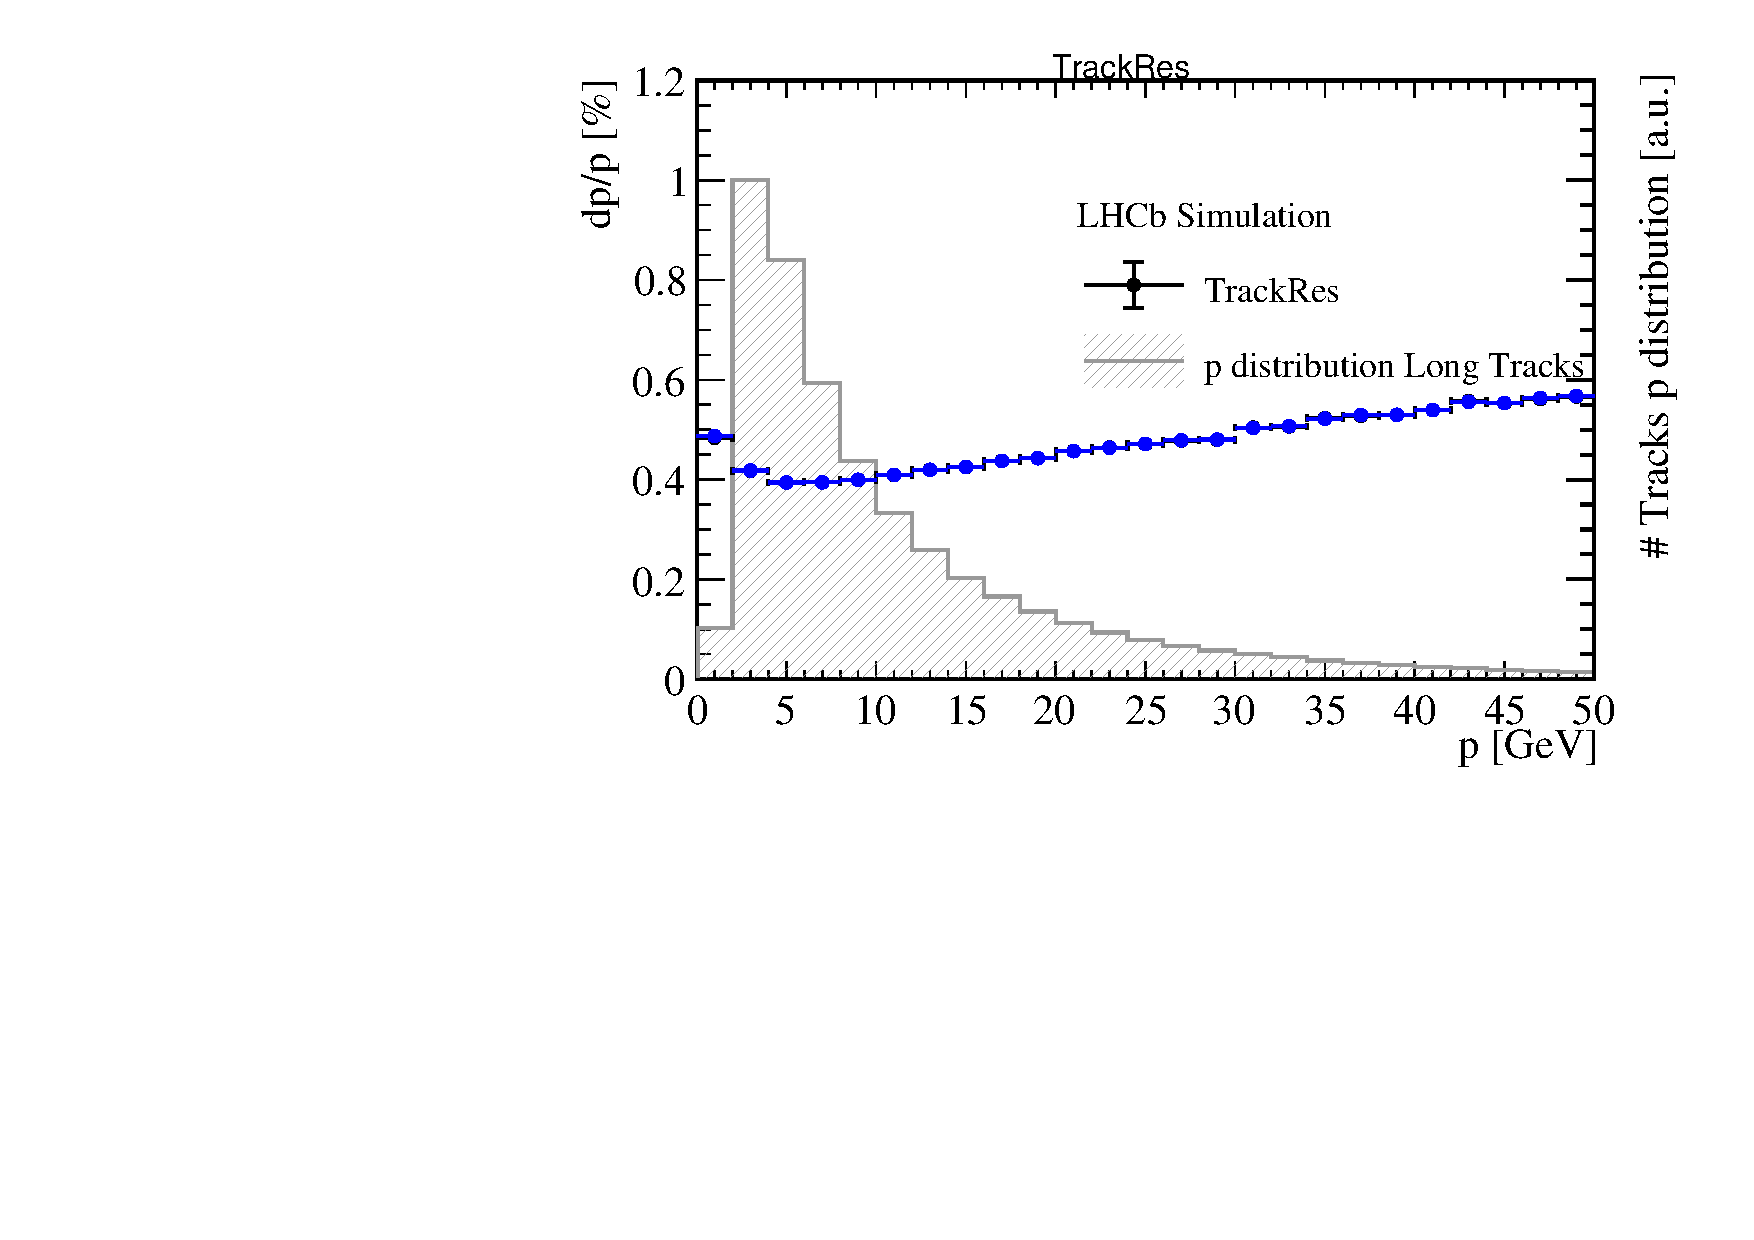
\includegraphics[width=1\textwidth]{Plots/Track_resolution_p_comparison.pdf}
    \end{subfigure}%
    \begin{subfigure}{0.50\textwidth}
      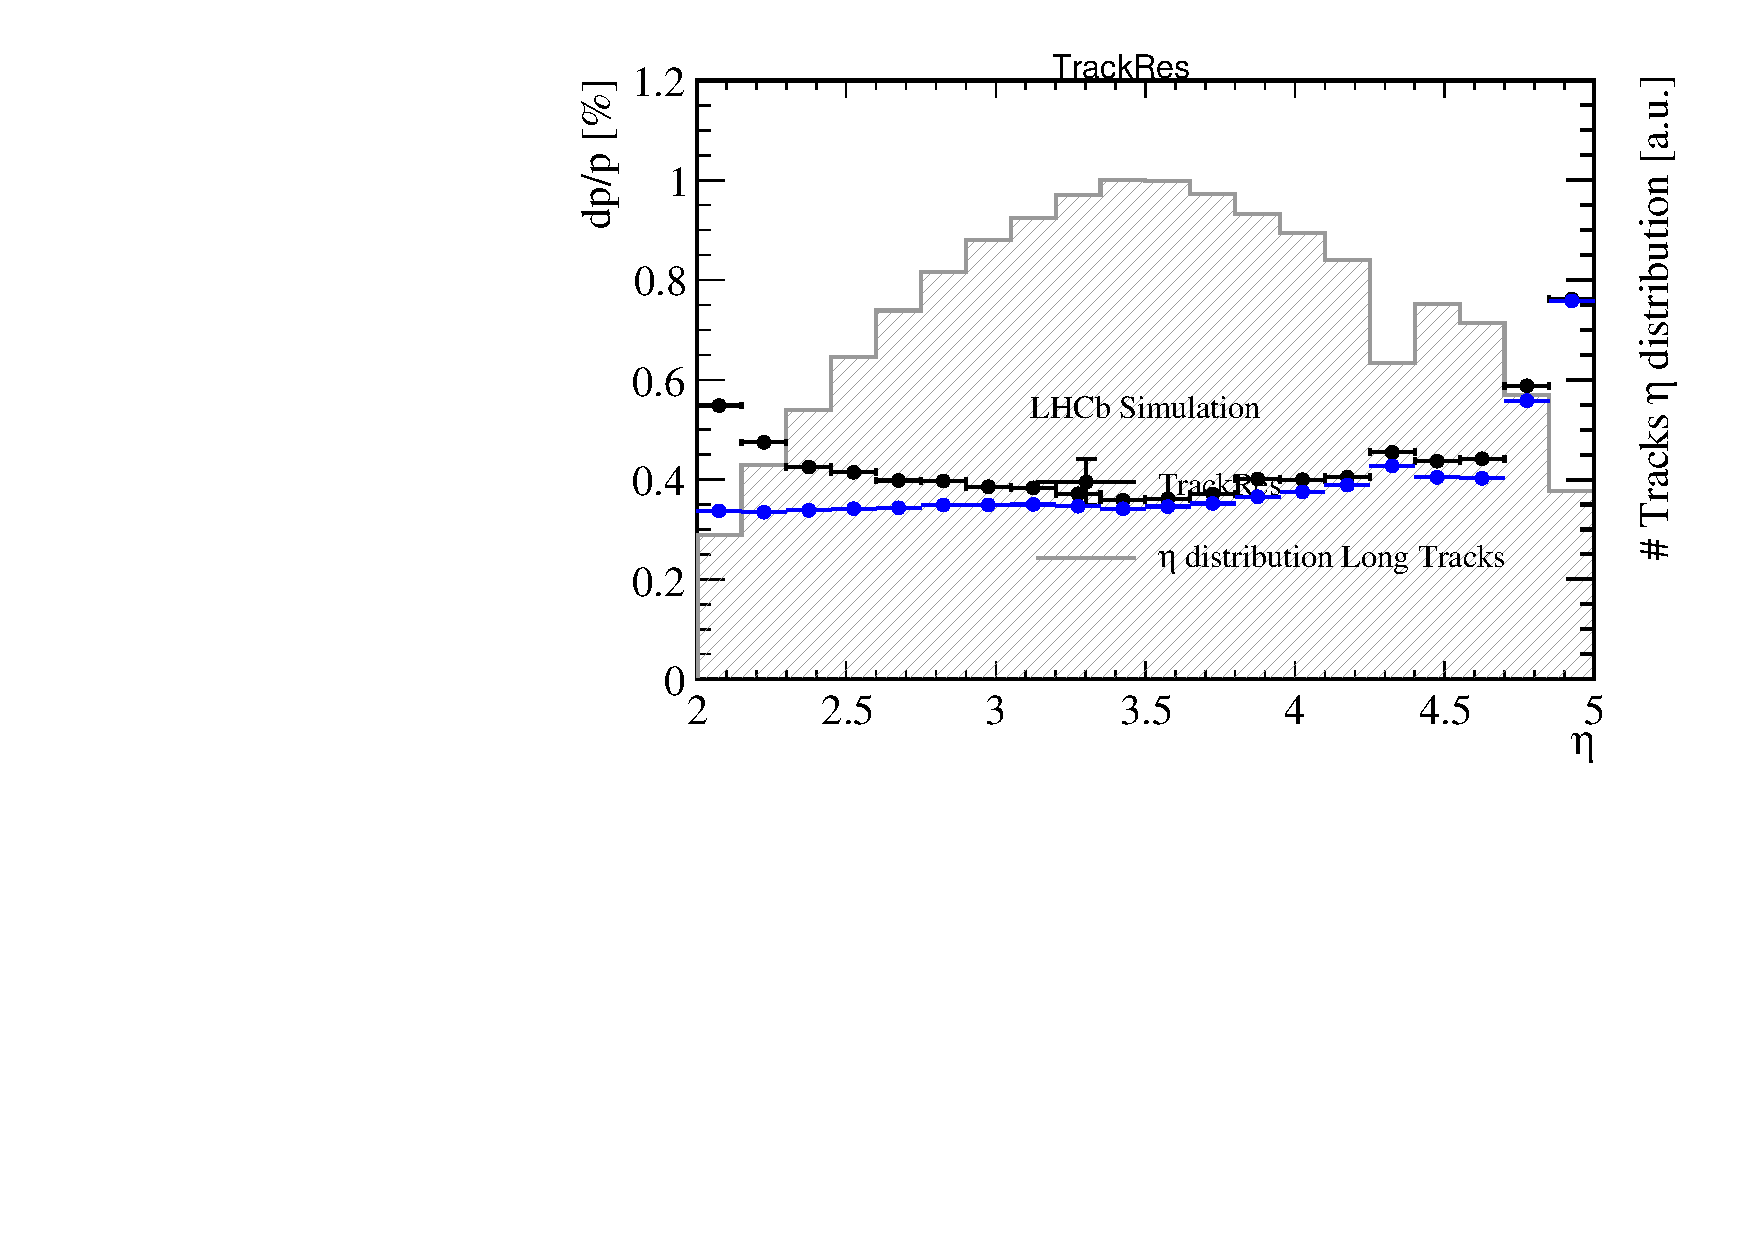
\includegraphics[width=1\textwidth]{Plots/Track_resolution_eta_comparison.pdf}
    \end{subfigure}
    \vspace{-0.2cm}
    \caption*{Black: Old parameterisation. {\color{blue}Blue: Updated parameterisation with old $z_{\rm mag}$}.}
  \end{figure}
  {\Large Clear improvement in momentum resolution!}
\end{frame}

\section{Closer study of \texorpdfstring{$z_{\rm mag}$}{zMag} parameterisation}

\begin{frame}{Study of $z_{\rm mag}$ bias}
  \vspace{0.0cm}
  {\Large Study bias $z_{\rm mag}^{\rm pred} - z_{\rm mag}$ of original parameterisation:}
  \begin{figure}[htb]
    \centering
    \begin{subfigure}{0.50\textwidth}
      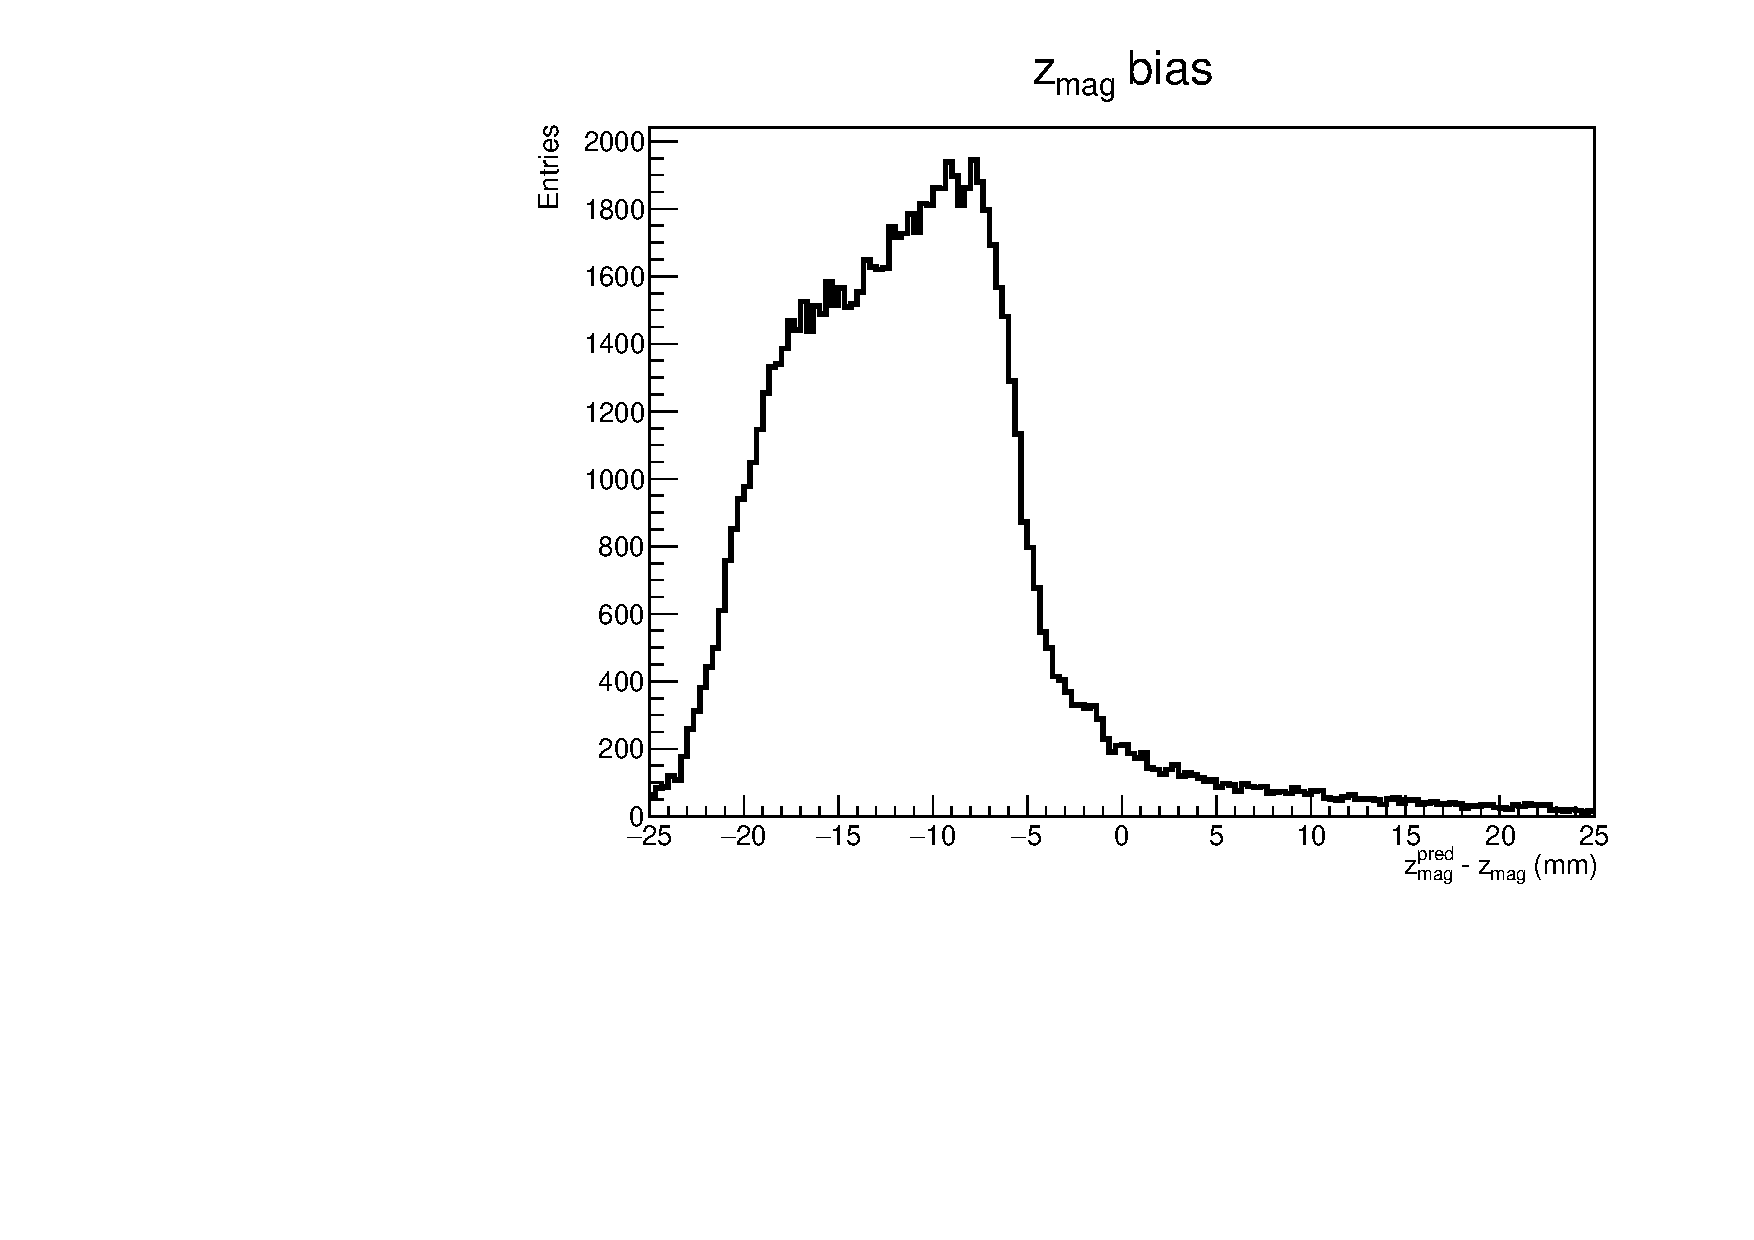
\includegraphics[width=1\textwidth]{Plots/z_mag_position_bias_old_parameterisation_low_p.pdf}
    \end{subfigure}%
    \begin{subfigure}{0.50\textwidth}
      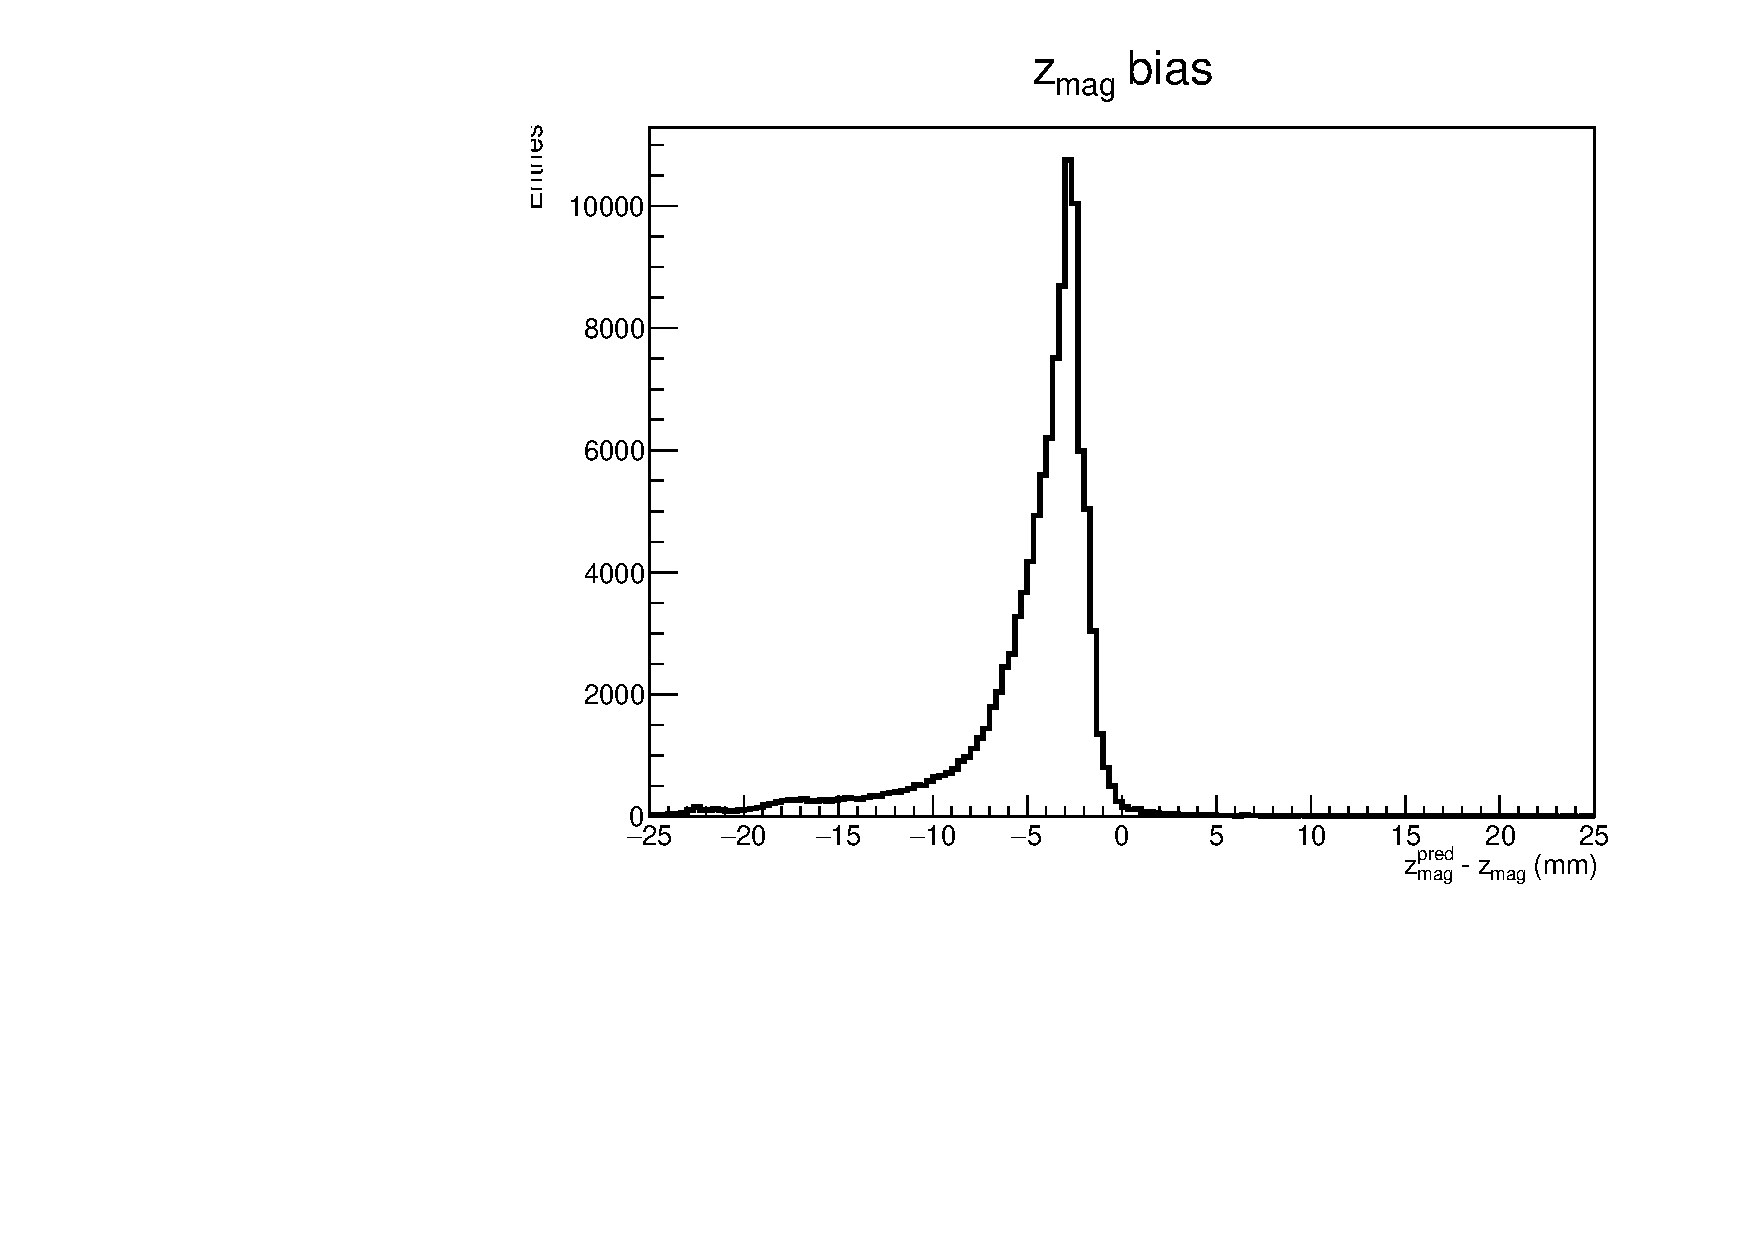
\includegraphics[width=1\textwidth]{Plots/z_mag_position_bias_old_parameterisation_high_p.pdf}
    \end{subfigure}
    \vspace{-0.2cm}
    \caption*{Left: $p < 7$~GeV. Right: $p > 7$~GeV.}
  \end{figure}
  \vspace{-0.5cm}
  \begin{itemize}
    \item{Parameterisation struggles a low momentum}
    \begin{itemize}
      \item[-]{Large negative bias}
      \item[-]{Very wide distribution}
    \end{itemize}
  \end{itemize}
\end{frame}

\begin{frame}{Study of $z_{\rm mag}$ bias}
  \vspace{0.0cm}
  {\Large Study bias $z_{\rm mag}^{\rm pred} - z_{\rm mag}$ of original parameterisation:}
  \begin{figure}[htb]
    \centering
    \begin{subfigure}{0.50\textwidth}
      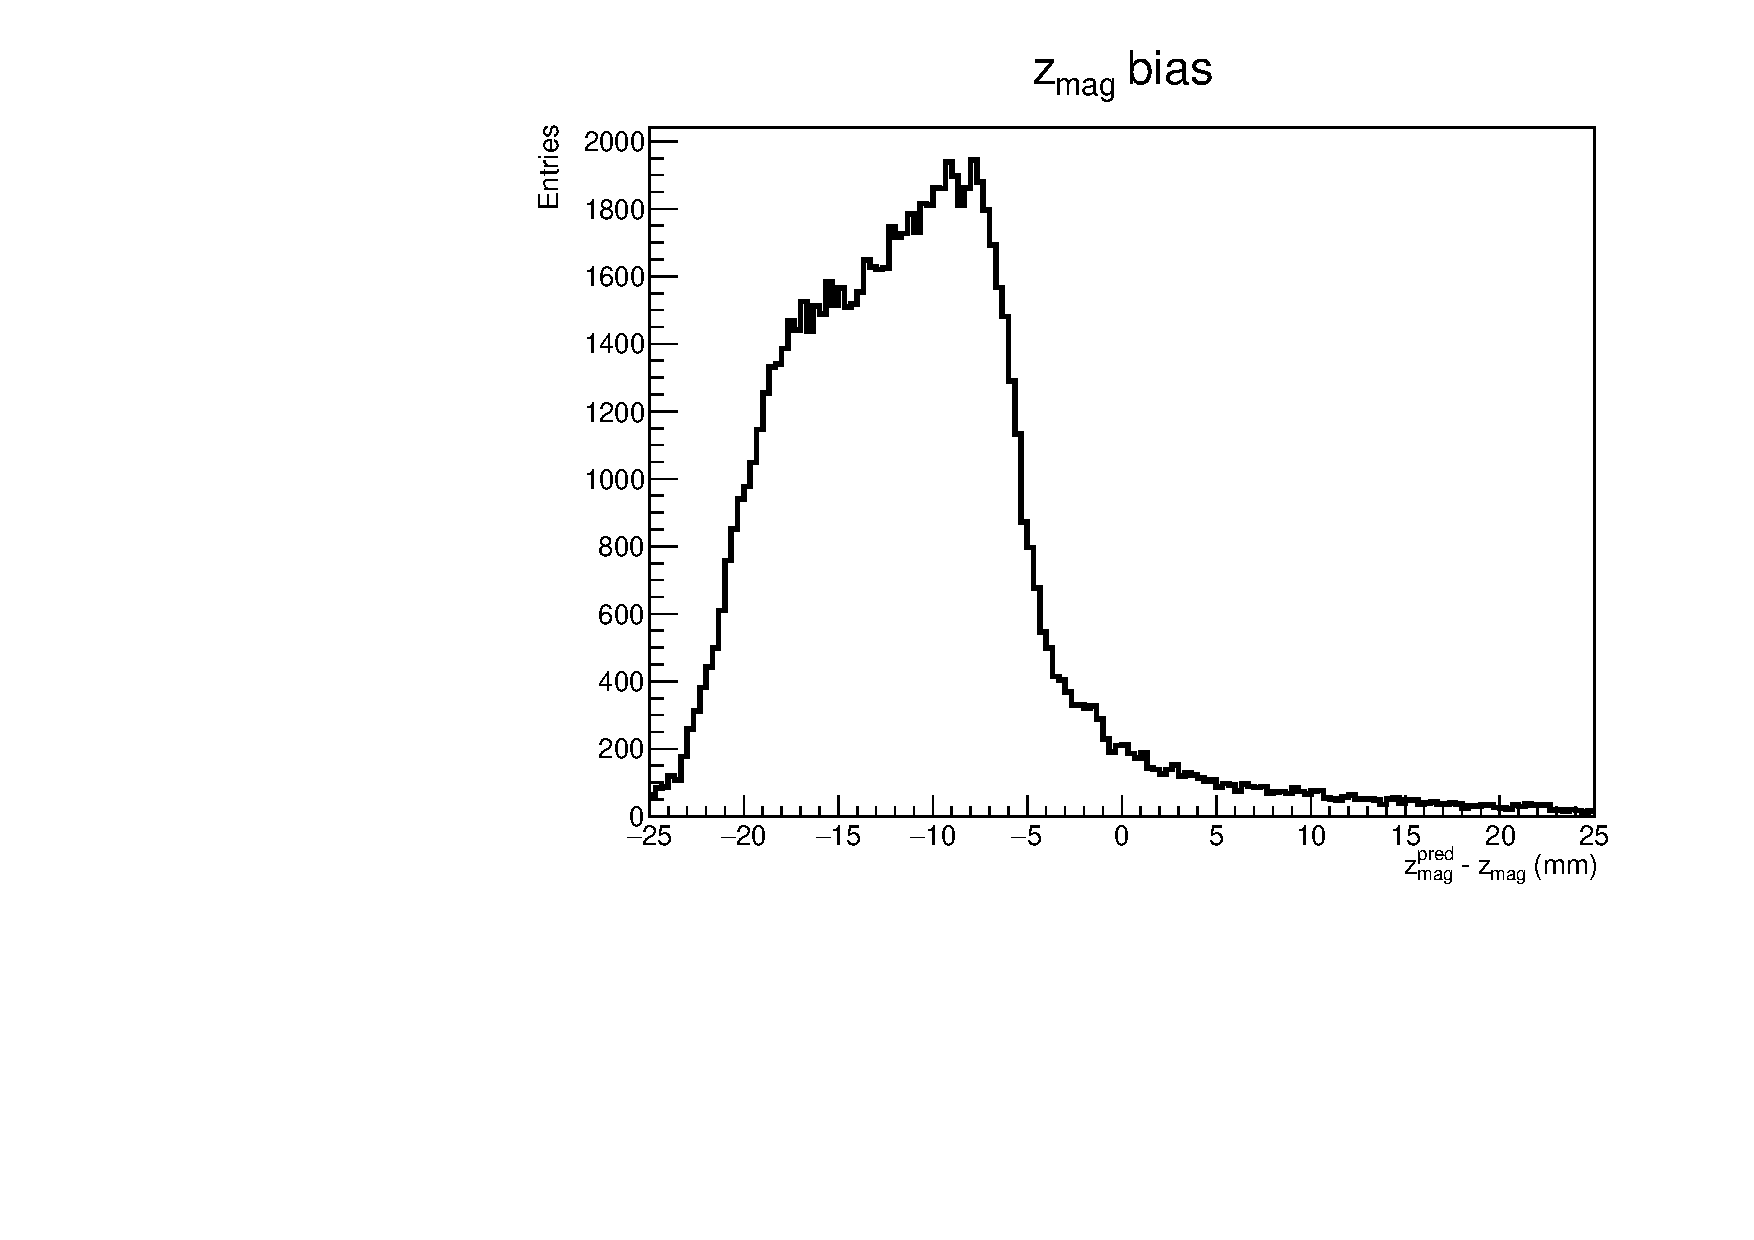
\includegraphics[width=1\textwidth]{Plots/z_mag_position_bias_old_parameterisation_low_p.pdf}
    \end{subfigure}%
    \begin{subfigure}{0.50\textwidth}
      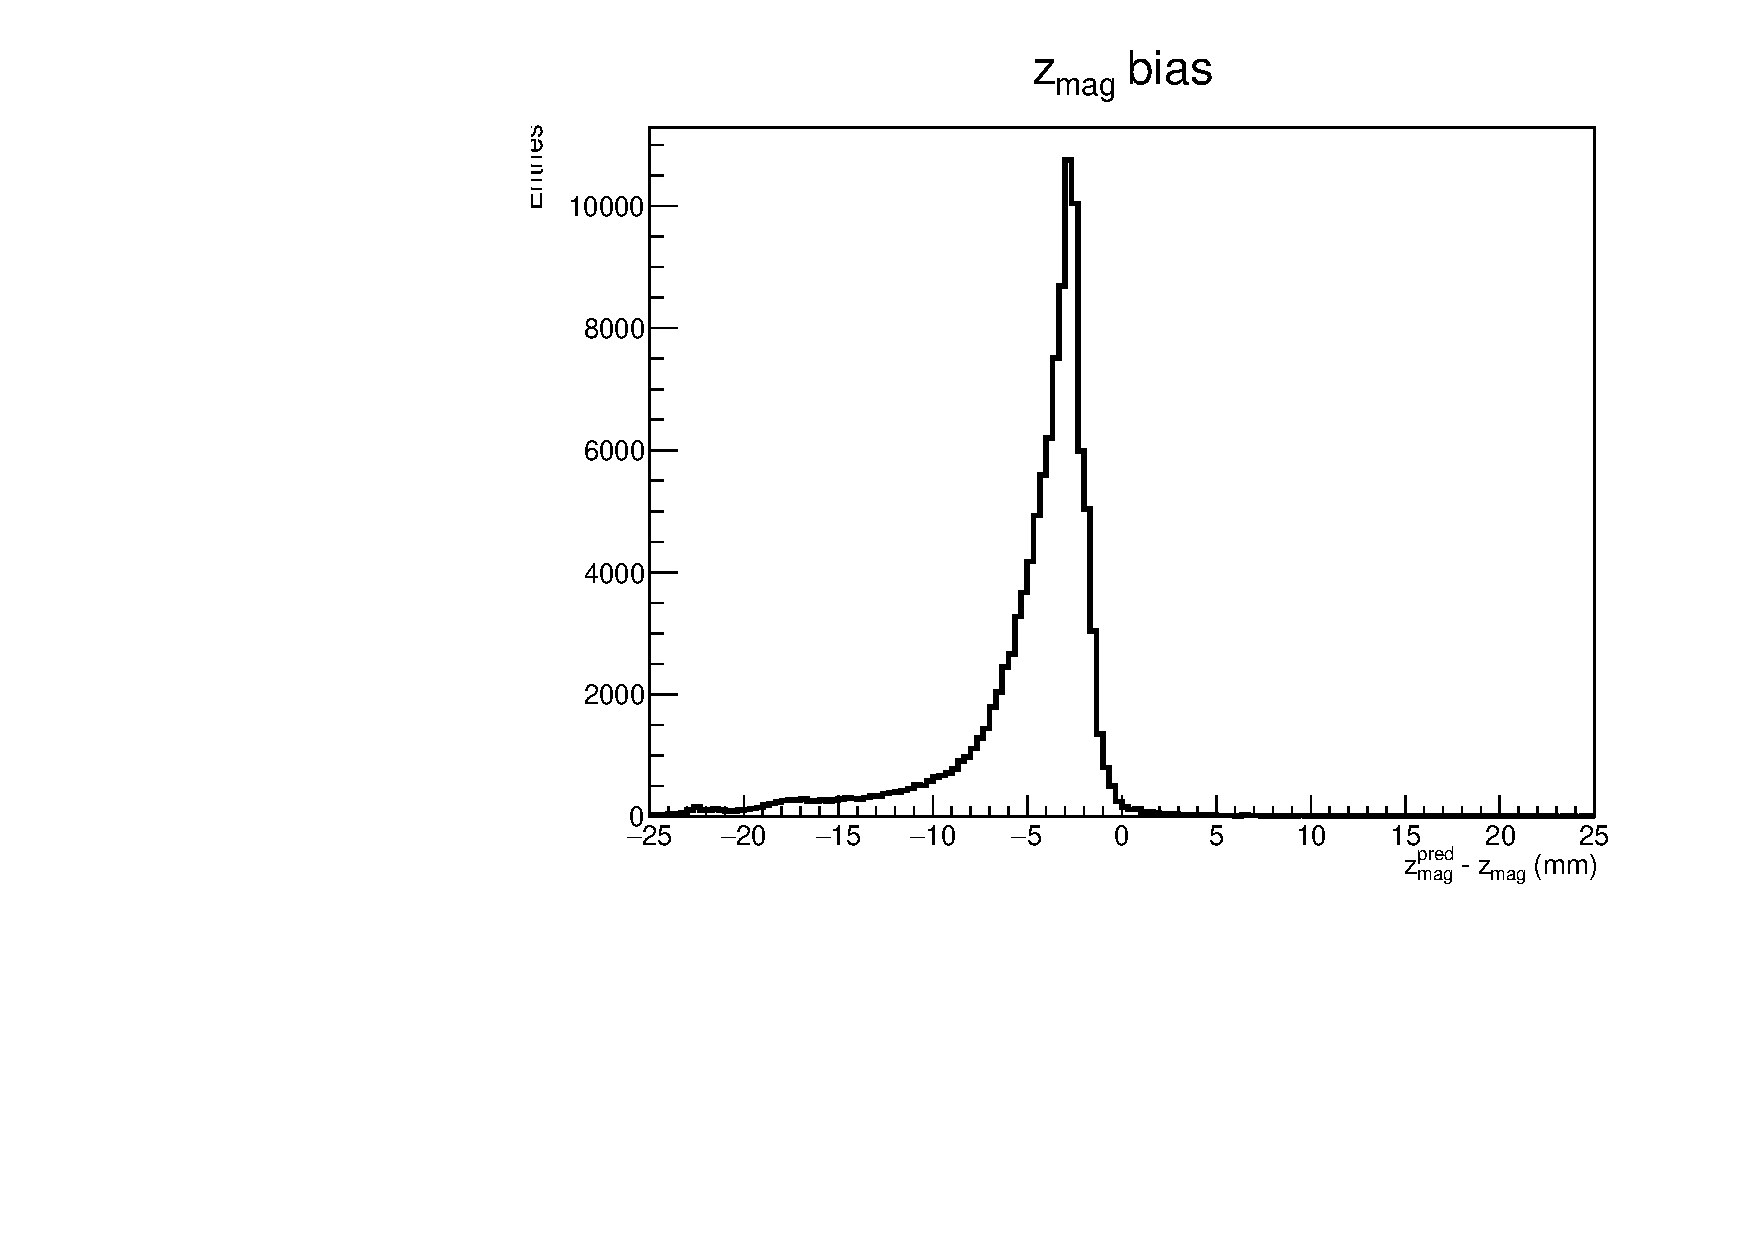
\includegraphics[width=1\textwidth]{Plots/z_mag_position_bias_old_parameterisation_high_p.pdf}
    \end{subfigure}
    \vspace{-0.2cm}
    \caption*{Left: $p < 7$~GeV. Right: $p > 7$~GeV.}
  \end{figure}
  \vspace{-0.5cm}
  \begin{itemize}
    \item{Parameterisation works well at high momentum}
    \begin{itemize}
      \item[-]{Small and almost negligible bias}
      \item[-]{Very small variance}
    \end{itemize}
  \end{itemize}
\end{frame}

\begin{frame}{Study of $z_{\rm mag}$ bias}
  \vspace{0.0cm}
  {\Large If we only update coefficients of $z_{\rm mag}$ parameterisation:}
  \begin{figure}[htb]
    \centering
    \begin{subfigure}{0.50\textwidth}
      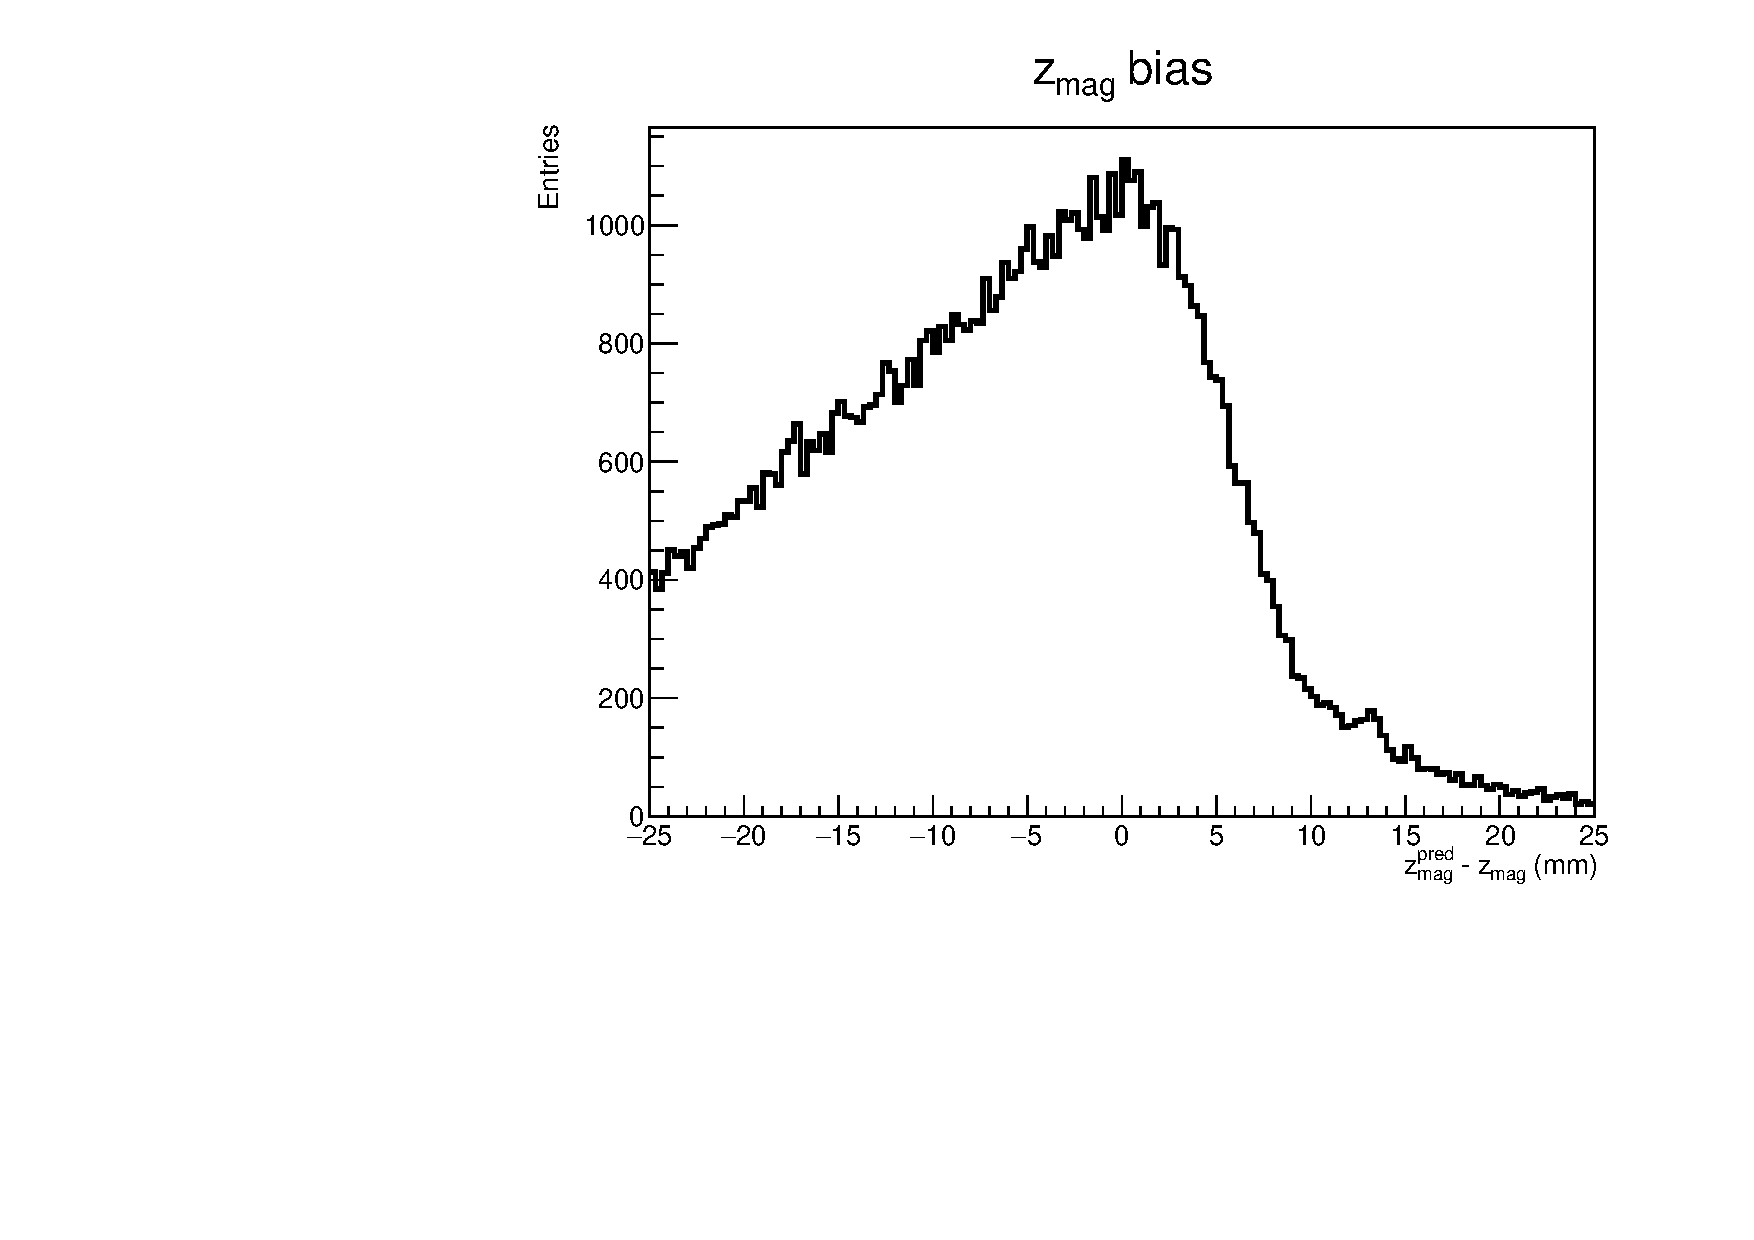
\includegraphics[width=1\textwidth]{Plots/z_mag_position_bias_bad_parameterisation_low_p.pdf}
    \end{subfigure}%
    \begin{subfigure}{0.50\textwidth}
      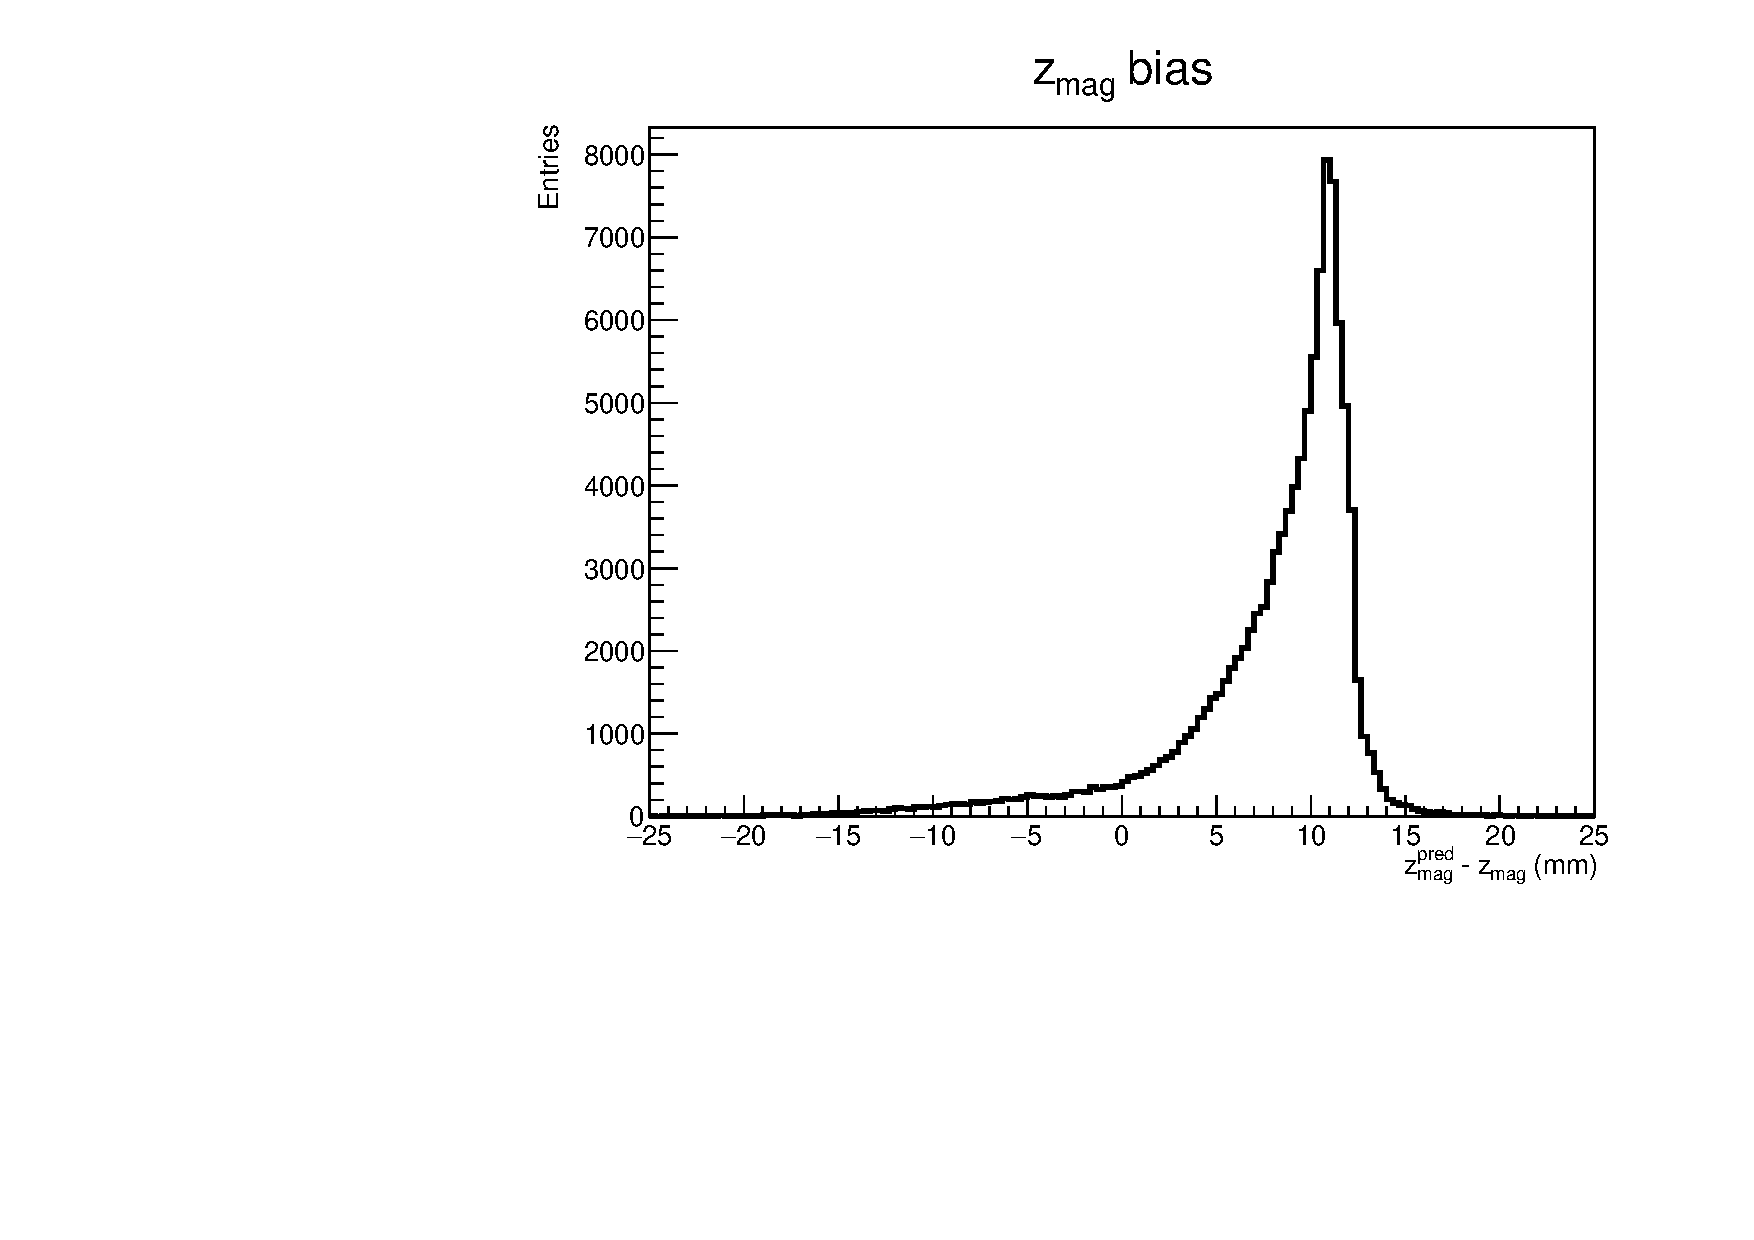
\includegraphics[width=1\textwidth]{Plots/z_mag_position_bias_bad_parameterisation_high_p.pdf}
    \end{subfigure}
    \vspace{-0.2cm}
    \caption*{Left: $p < 7$~GeV. Right: $p > 7$~GeV.}
  \end{figure}
  \vspace{-0.5cm}
  \begin{itemize}
    \item{Potential explanation of worse performance with new coefficients:}
    \begin{itemize}
      \item[-]{Bias is generally worse}
      \item[-]{Parameterisation doesn't describe $z_{\rm mag}$ well}
    \end{itemize}
  \end{itemize}
\end{frame}

\begin{frame}{Reminder: $z_{\rm mag}$ parameterisation}
  \vspace{0.0cm}
  \begin{figure}[htb]
    \centering
    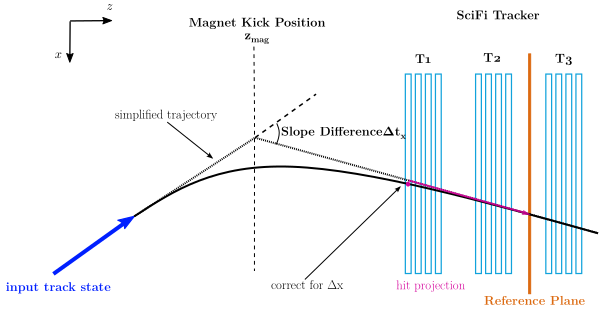
\includegraphics[width=0.75\textwidth]{Plots/MagnetKinkPosition.png}
    \caption*{\small From CERN-THESIS-2023-097}
  \end{figure}

  \begin{itemize}
    \item{Original $z_{\rm mag}$ parameterisation:}
  \end{itemize}
  \begin{align*}
    z_{\rm mag} =& c_0 + c_1t_x^2 + c_3t_y^2 + \Delta t_x^\prime(c_2t_x + c_4\Delta t_x^\prime) \\
  \end{align*}
\end{frame}

\begin{frame}{Improved $z_{\rm mag}$ parameterisation}
  \vspace{0.0cm}
  \begin{figure}[htb]
    \centering
    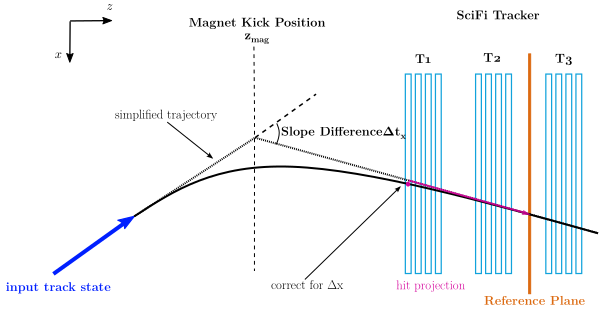
\includegraphics[width=0.75\textwidth]{Plots/MagnetKinkPosition.png}
    \caption*{\small From CERN-THESIS-2023-097}
  \end{figure}
  \begin{itemize}
    \item{After trial and error, this parameterisation was obtained:}
  \end{itemize}
  \begin{align*}
    z_{\rm mag} =& c_0 + c_1t_x^2 + c_3t_y^2 + \Delta t_x^\prime(c_2t_x + c_4\Delta t_x^\prime) \\
    +& (c_5 + tx^2 + ty^2 + \lvert\Delta t_x^\prime\rvert^2)\lvert\Delta t_x^\prime\rvert
  \end{align*}
\end{frame}

\begin{frame}{Study of $z_{\rm mag}$ bias}
  \vspace{0.0cm}
  {\Large Check biases with new improved parameterisation:}
  \begin{figure}[htb]
    \centering
    \begin{subfigure}{0.50\textwidth}
      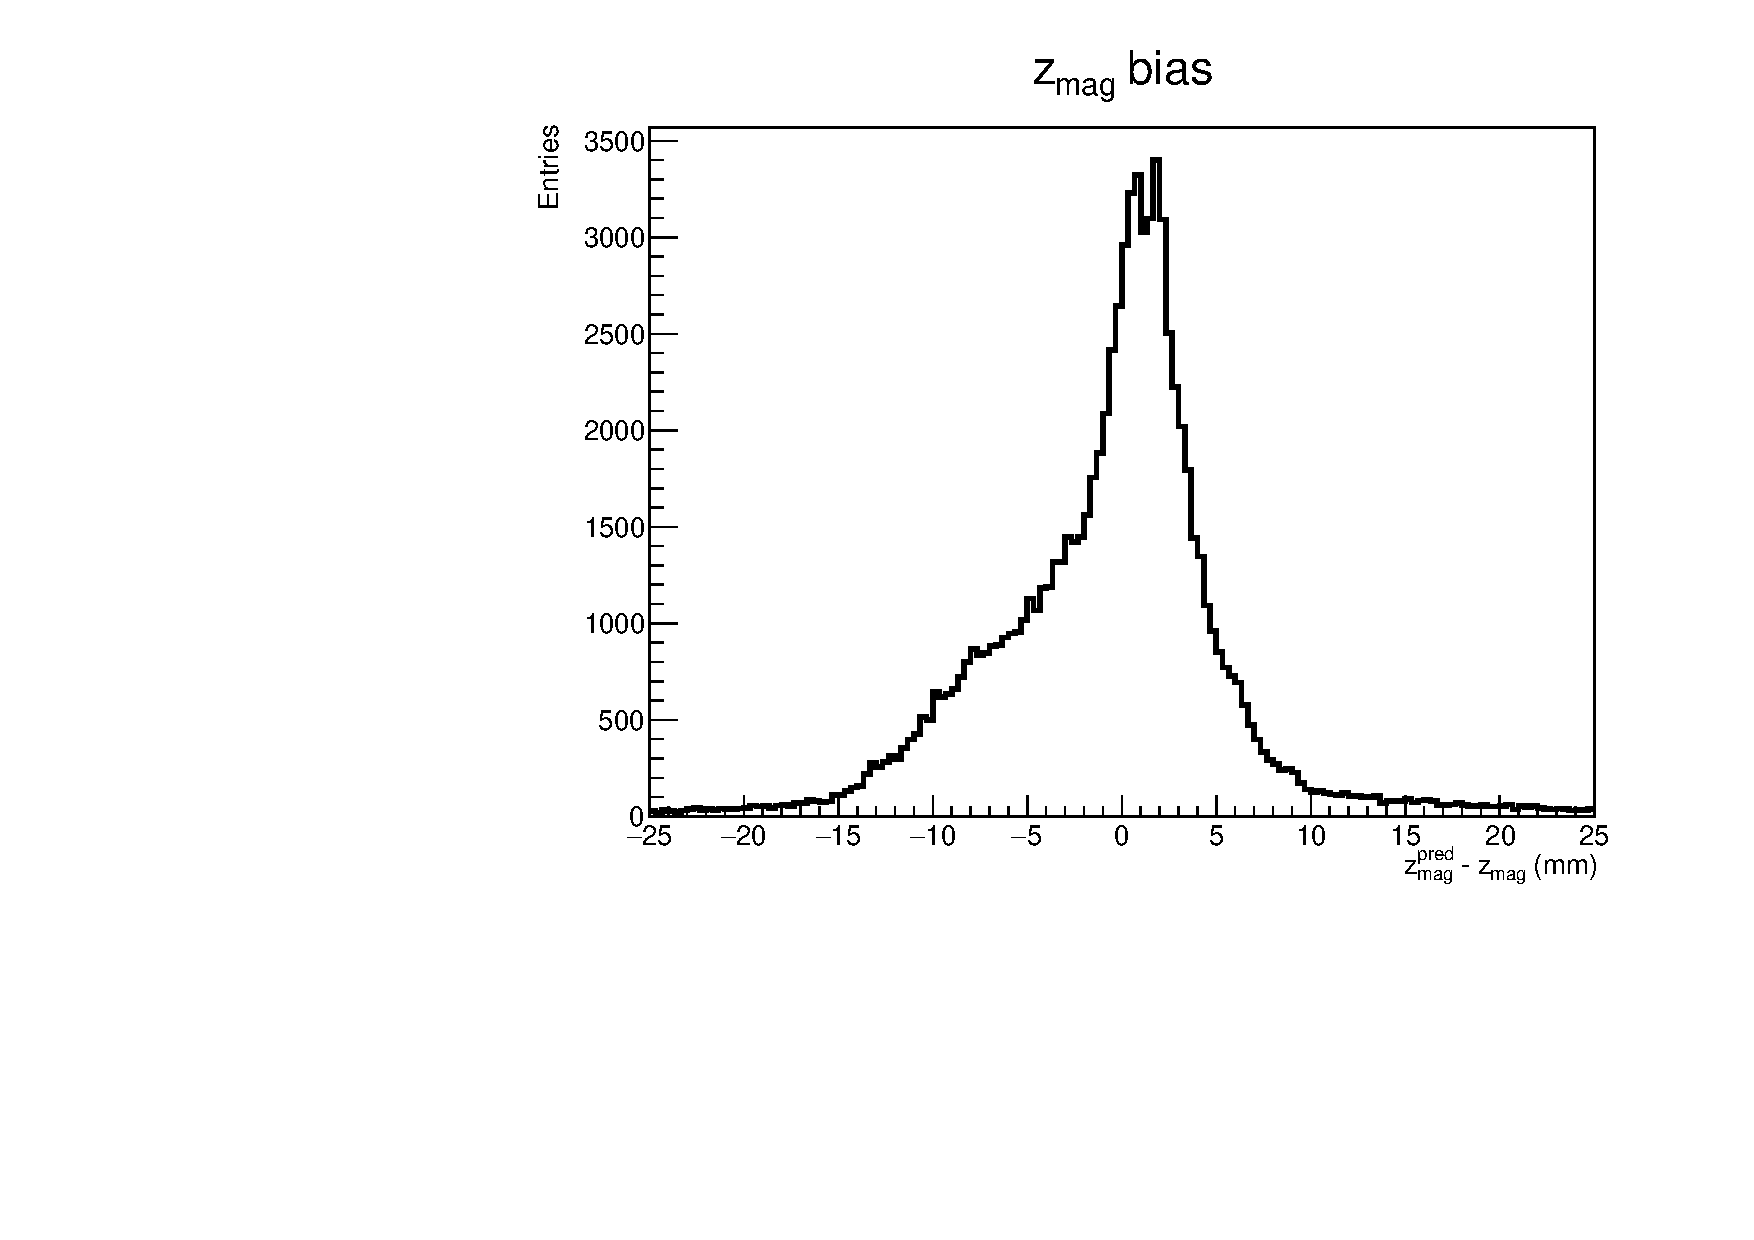
\includegraphics[width=1\textwidth]{Plots/z_mag_position_bias_new_parameterisation_low_p.pdf}
    \end{subfigure}%
    \begin{subfigure}{0.50\textwidth}
      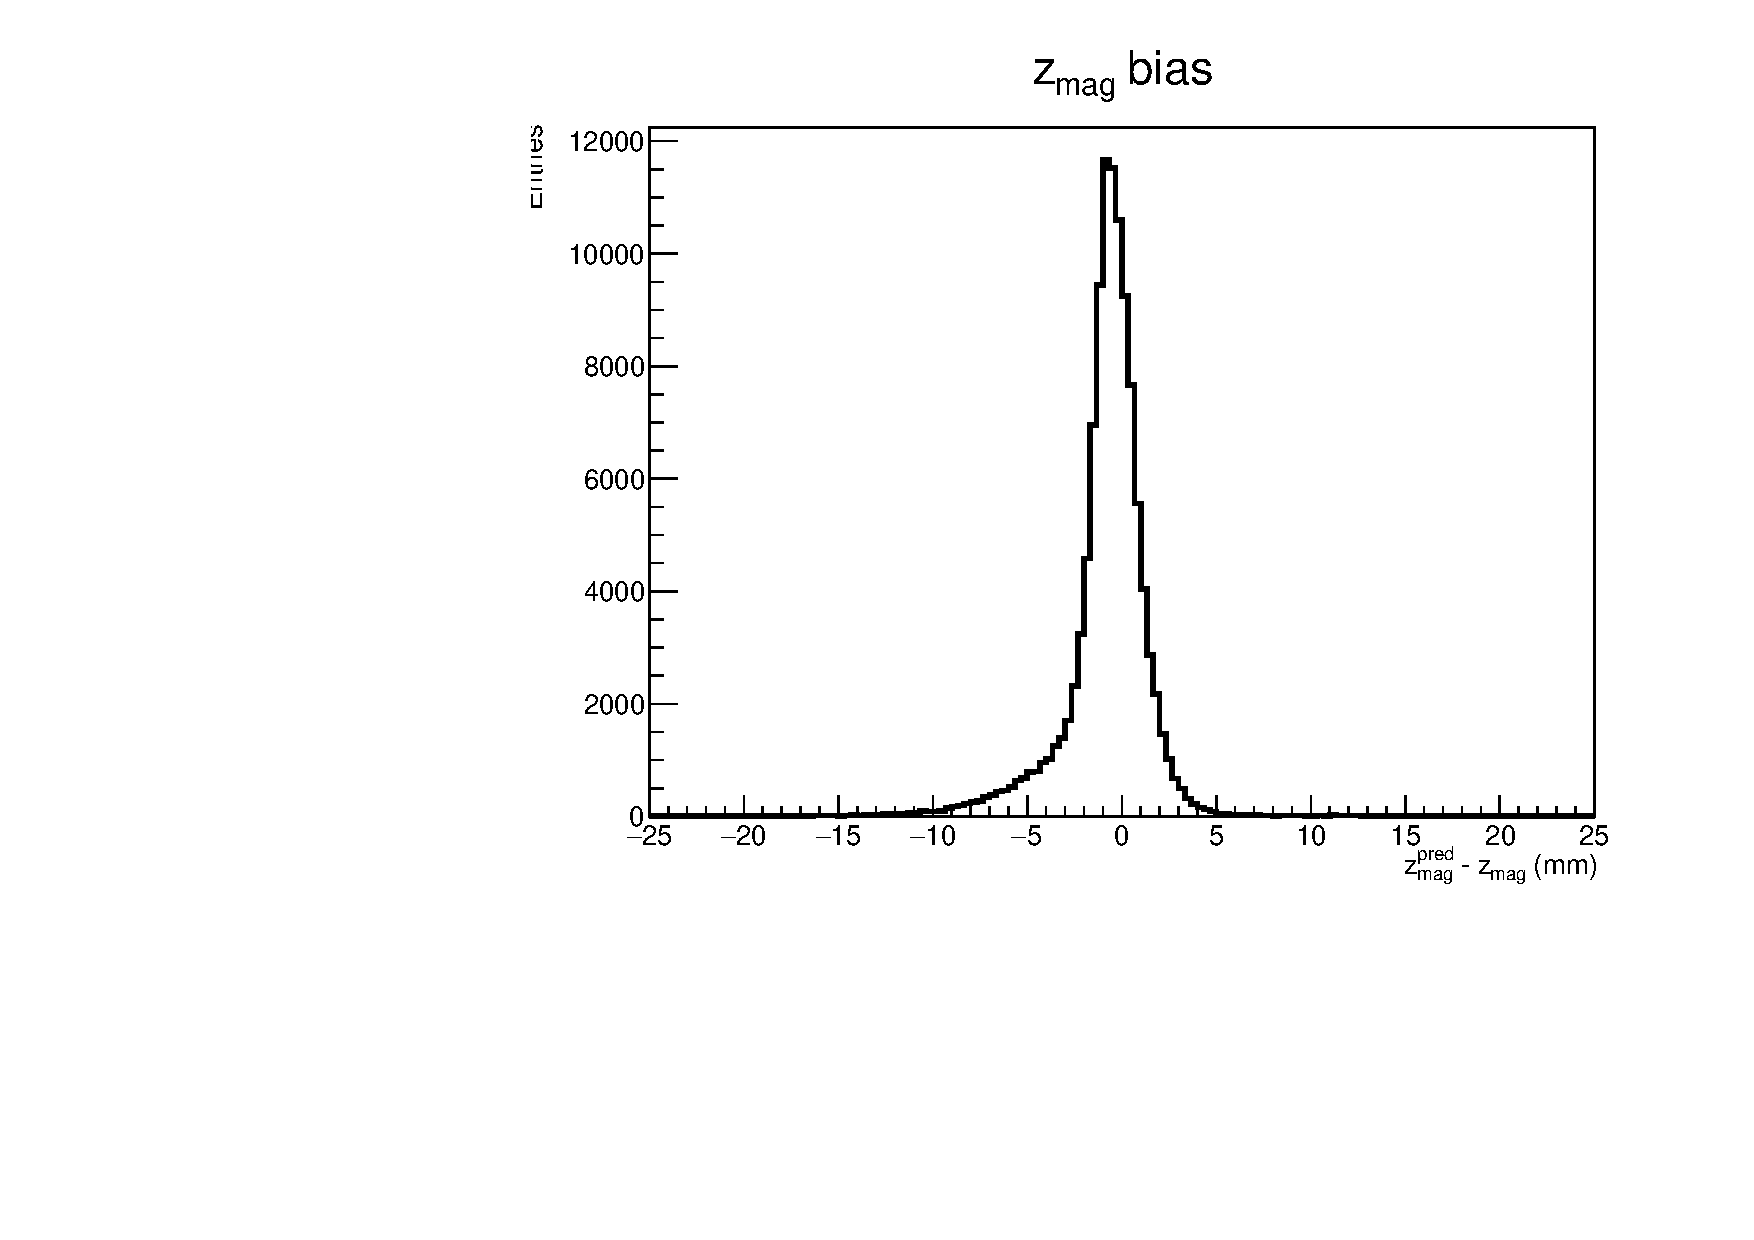
\includegraphics[width=1\textwidth]{Plots/z_mag_position_bias_new_parameterisation_high_p.pdf}
    \end{subfigure}
    \vspace{-0.2cm}
    \caption*{Left: $p < 7$~GeV. Right: $p > 7$~GeV.}
  \end{figure}
  \vspace{-0.5cm}
  \begin{itemize}
    \item{Huge improvement in biases:}
    \begin{itemize}
      \item[-]{Almost symmetric and unbiased distribution at high momentum}
      \item[-]{Mostly unbiased at low momentum, with a left tail}
    \end{itemize}
  \end{itemize}
\end{frame}

\begin{frame}{Tracking efficiencies with new improved parameterisation}
  \vspace{0.0cm}
  \begin{figure}[htb]
    \centering
    \begin{subfigure}{0.45\textwidth}
      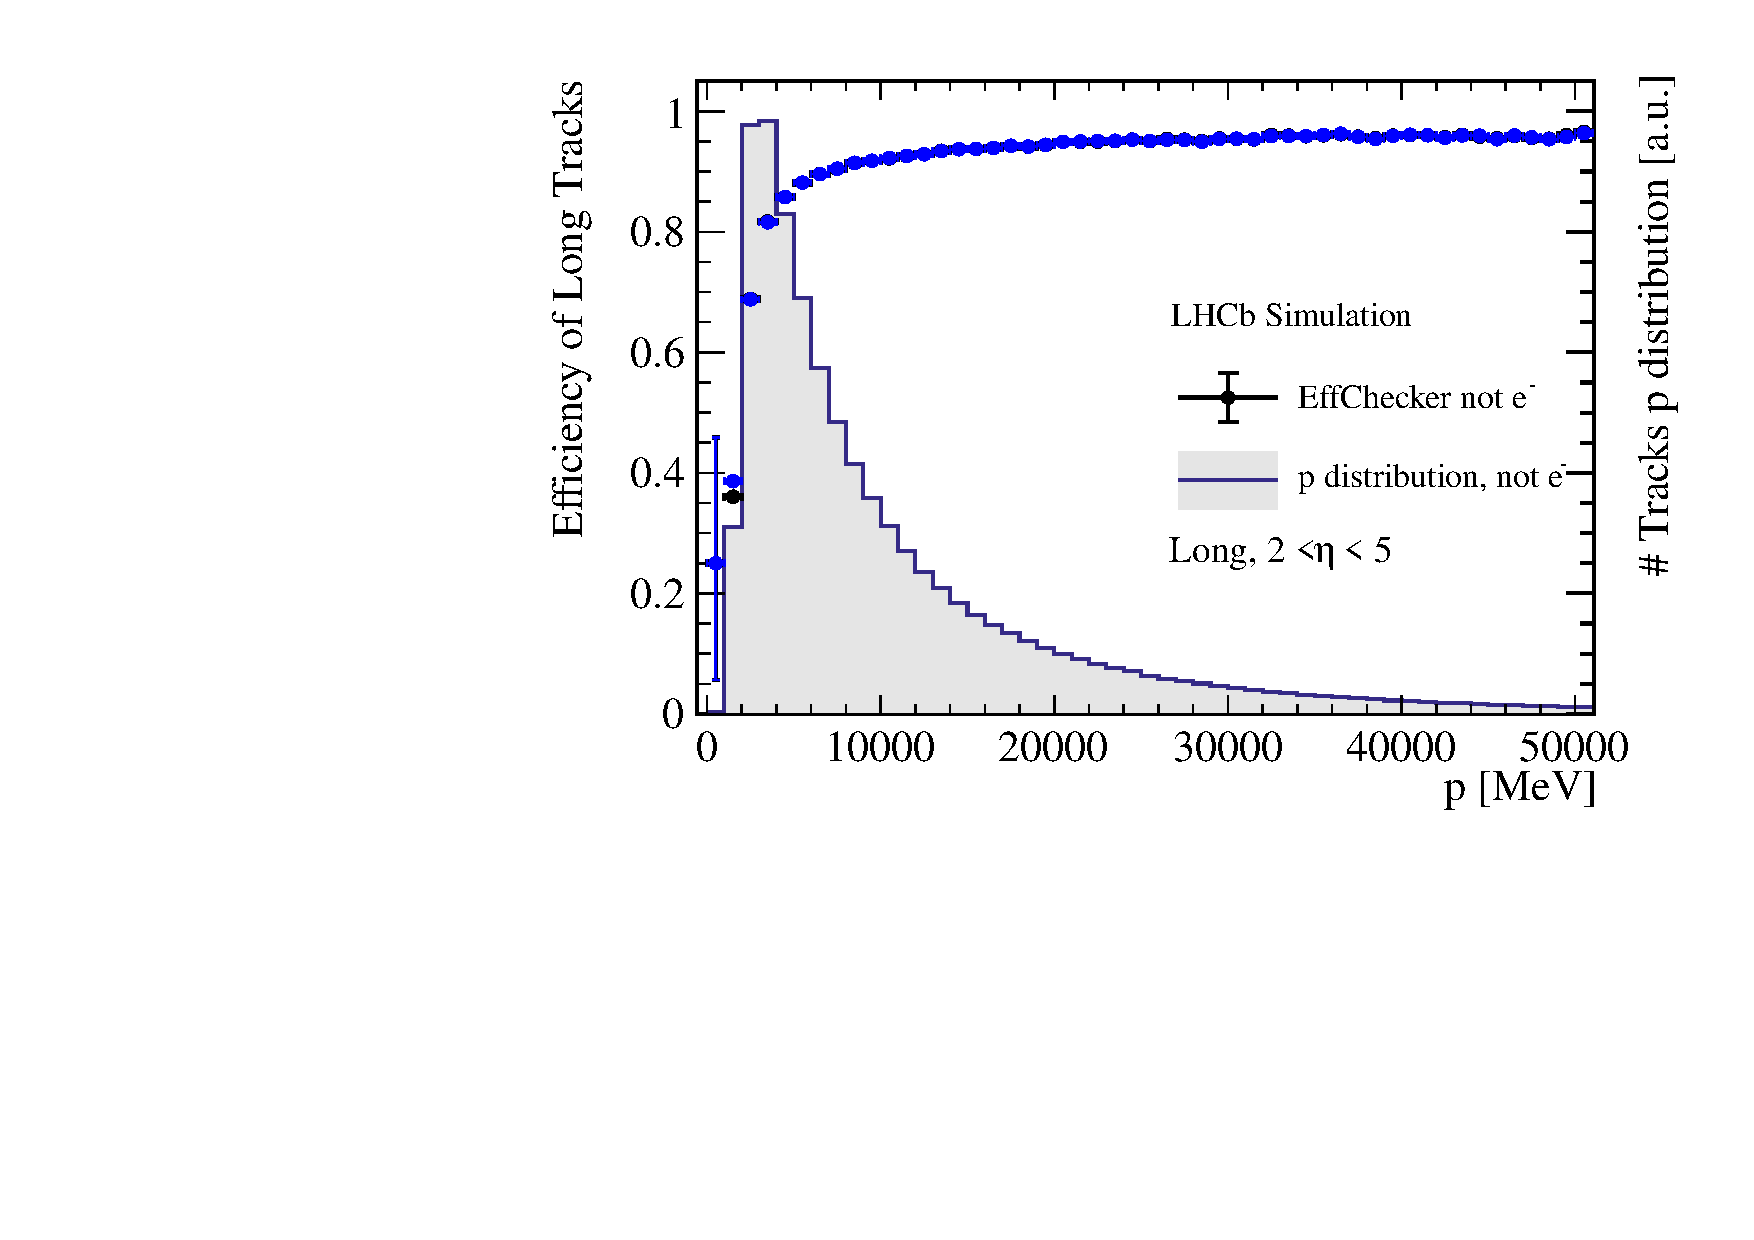
\includegraphics[width=1\textwidth]{Plots/TrackEfficiency_p_improved_MC_parameterisation.pdf}
    \end{subfigure}%
    \begin{subfigure}{0.45\textwidth}
      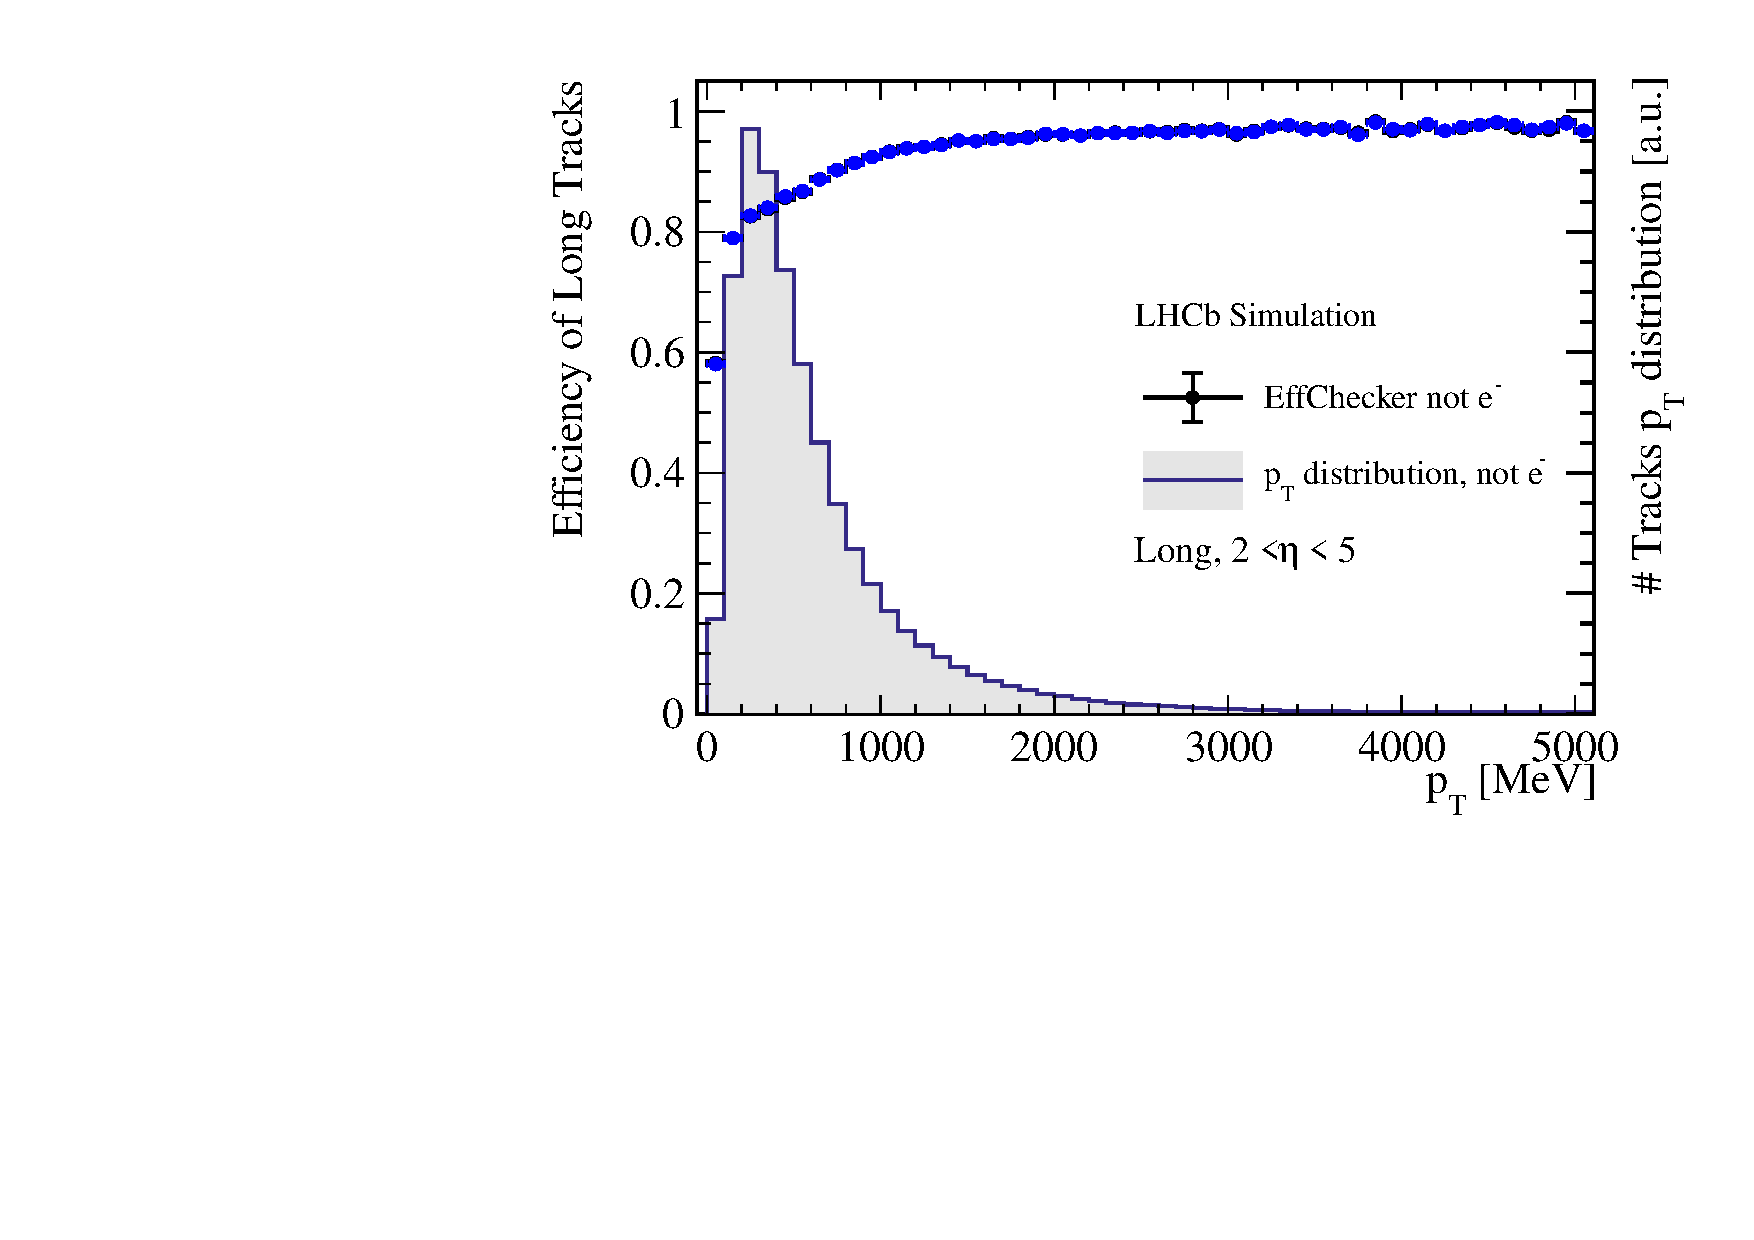
\includegraphics[width=1\textwidth]{Plots/TrackEfficiency_pt_improved_MC_parameterisation.pdf}
    \end{subfigure}
    \begin{subfigure}{0.45\textwidth}
      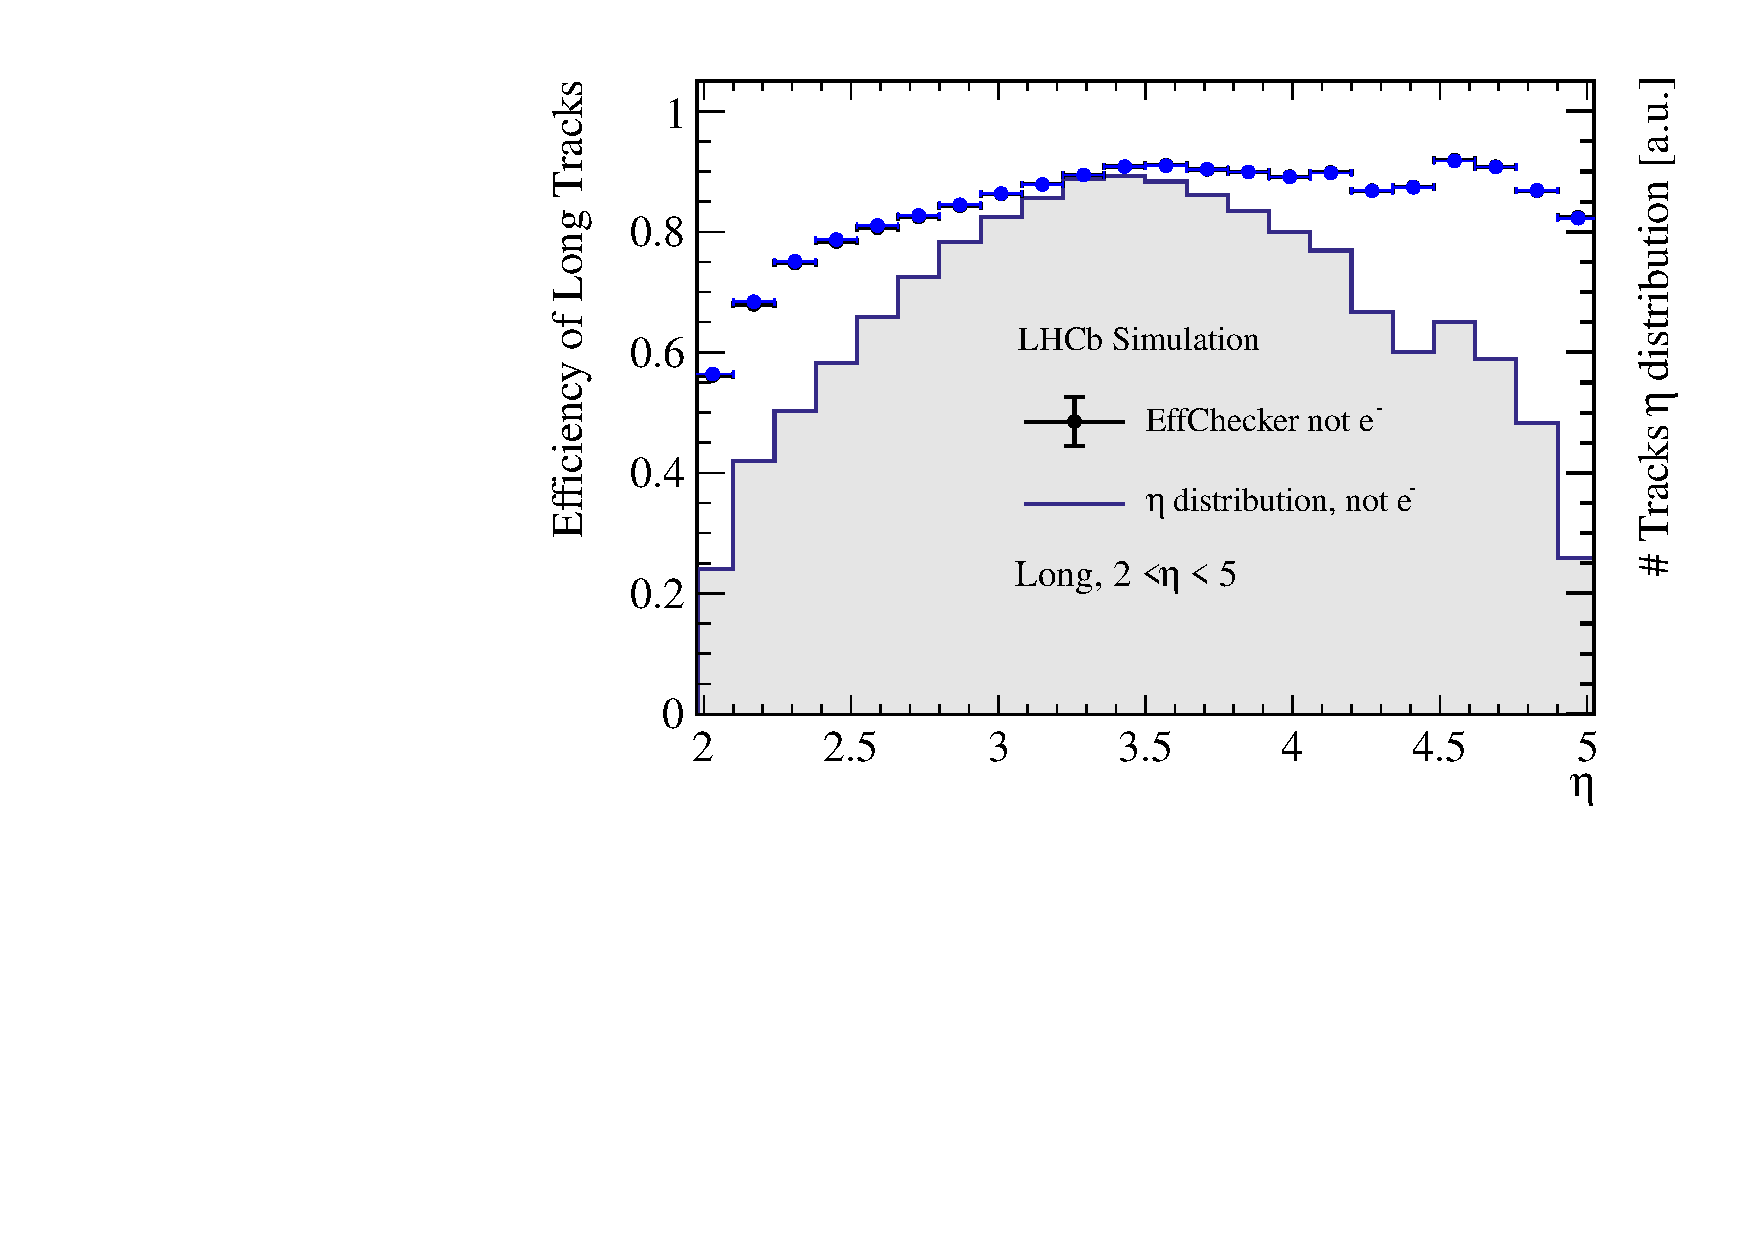
\includegraphics[width=1\textwidth]{Plots/TrackEfficiency_eta_improved_MC_parameterisation.pdf}
    \end{subfigure}%
    \begin{subfigure}{0.45\textwidth}
      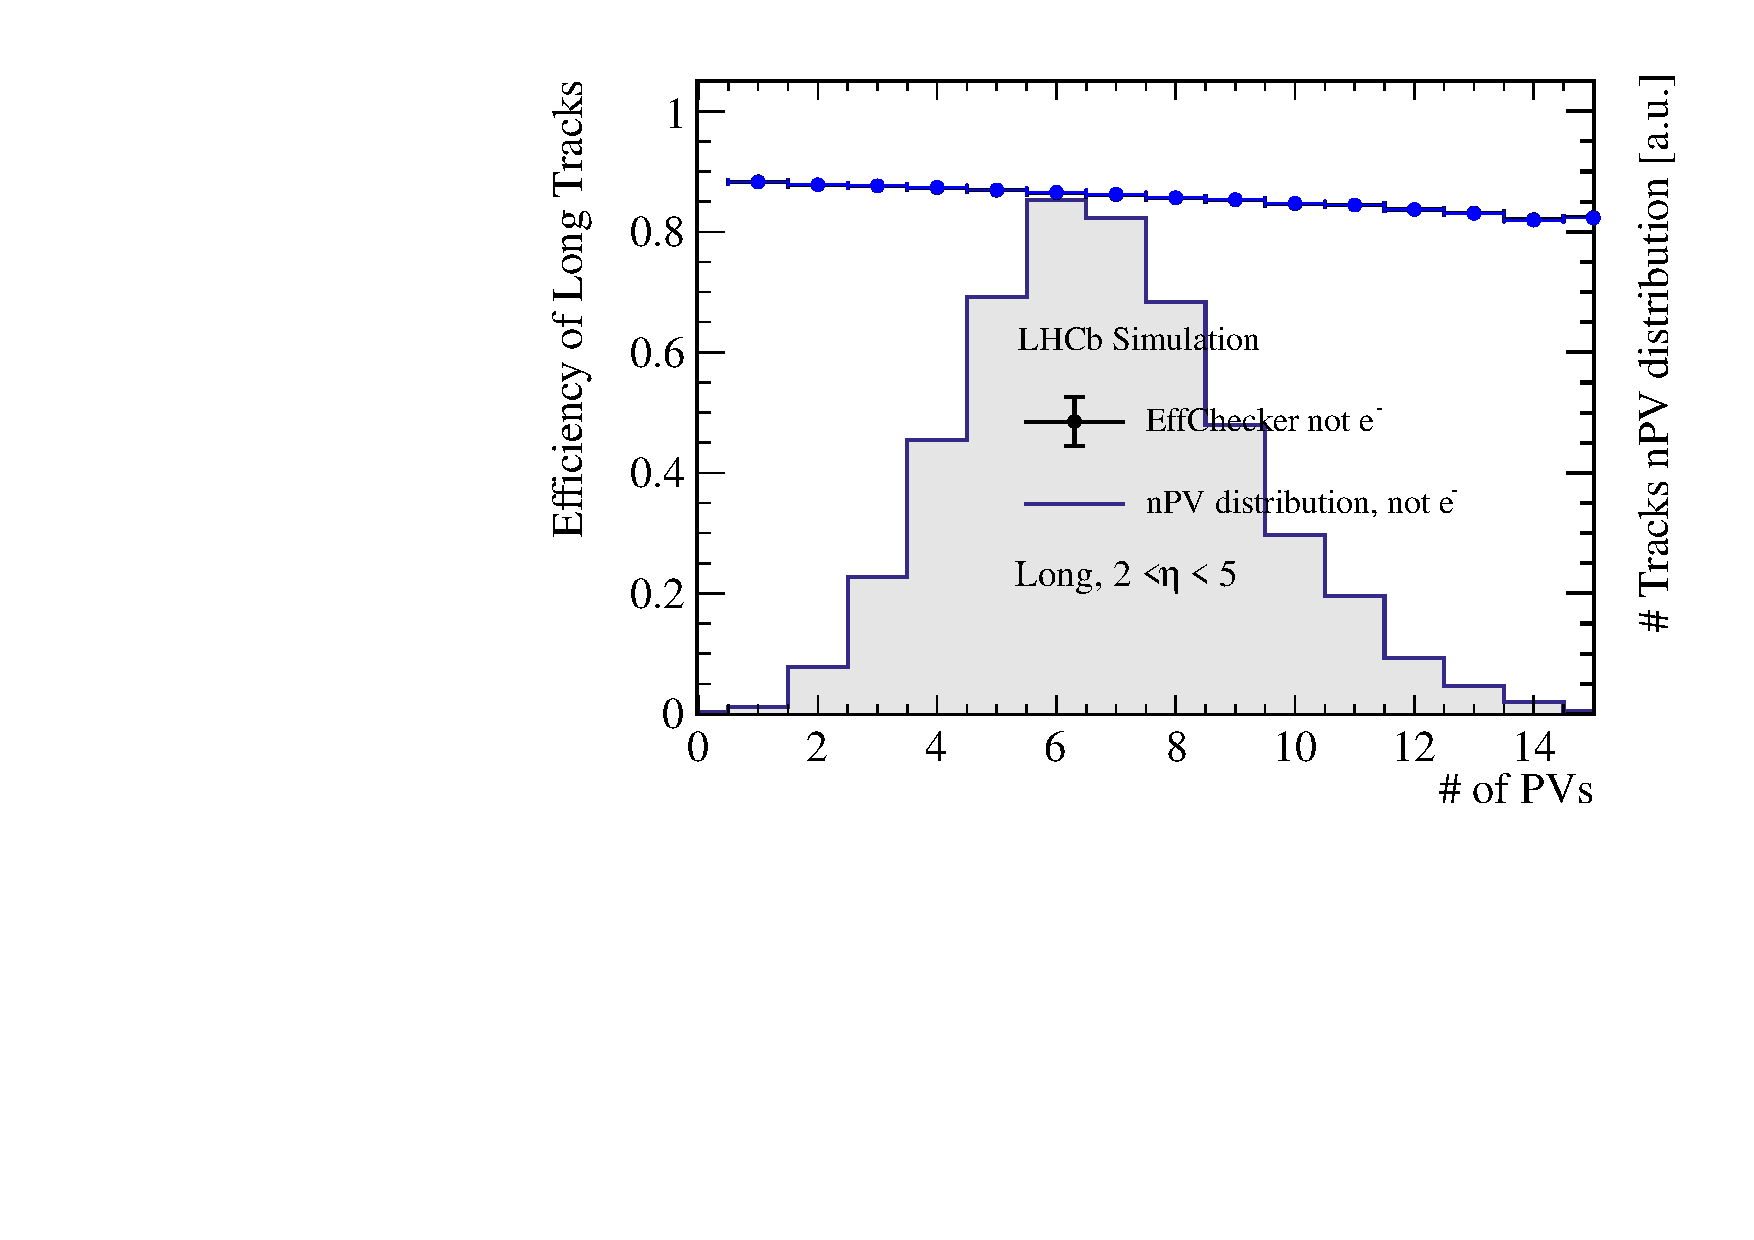
\includegraphics[width=1\textwidth]{Plots/TrackEfficiency_nPV_improved_MC_parameterisation.pdf}
    \end{subfigure}
    \vspace{-0.2cm}
    \caption*{Black: Old parameterisation. {\color{blue}Blue: Improved parameterisation of $z_{\rm mag}$} {\color{red}need to update these plots}.}
  \end{figure}
\end{frame}

\begin{frame}{Tracking efficiencies with new improved parameterisation}
  \vspace{0.0cm}
  \begin{itemize}
    \setlength\itemsep{1.0em}
    \item{I propose that we keep the original $z_{\rm mag}$ parameterisation}
    \begin{itemize}
      \item{Determined by Andre G{\"u}nther using DC19 MC}
    \end{itemize}
    \item{Somehow, tracking efficiencies get \underline{worse} when using a more accurate parameterisation...}
    \item{...but perhaps in this case doing the wrong thing is better}
    \item{Is there a straightforward explanation for this...?}
  \end{itemize}
\end{frame}

\begin{frame}{Reminder: Hit mapping to reference plane}
  \vspace{0.0cm}
  \begin{figure}[htb]
    \centering
    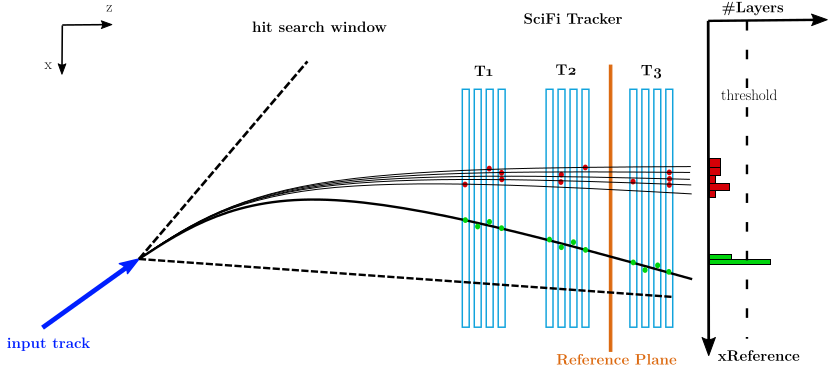
\includegraphics[width=0.8\textwidth]{Plots/HoughTransform.png}
  \caption*{\small From CERN-THESIS-2023-097}
  \end{figure}
  \vspace{-0.3cm}
  \begin{itemize}
    \item{Define a search window by assuming $p = p_{\rm min} = 1500$~MeV/c}
    \item{My understanding is:}
    \begin{itemize}
      \item[-]{$z_{\rm mag}$ is underestimated $\to$ Search window becomes larger!}
      \item[-]{$\to$ Add negative bias at low momentum to improve performance}
    \end{itemize}
  \end{itemize}
\end{frame}

\begin{frame}{Tracking efficiencies with biased $z_{\rm mag}$ parameterisation}
  \vspace{0.0cm}
  \begin{figure}[htb]
    \centering
    \begin{subfigure}{0.45\textwidth}
      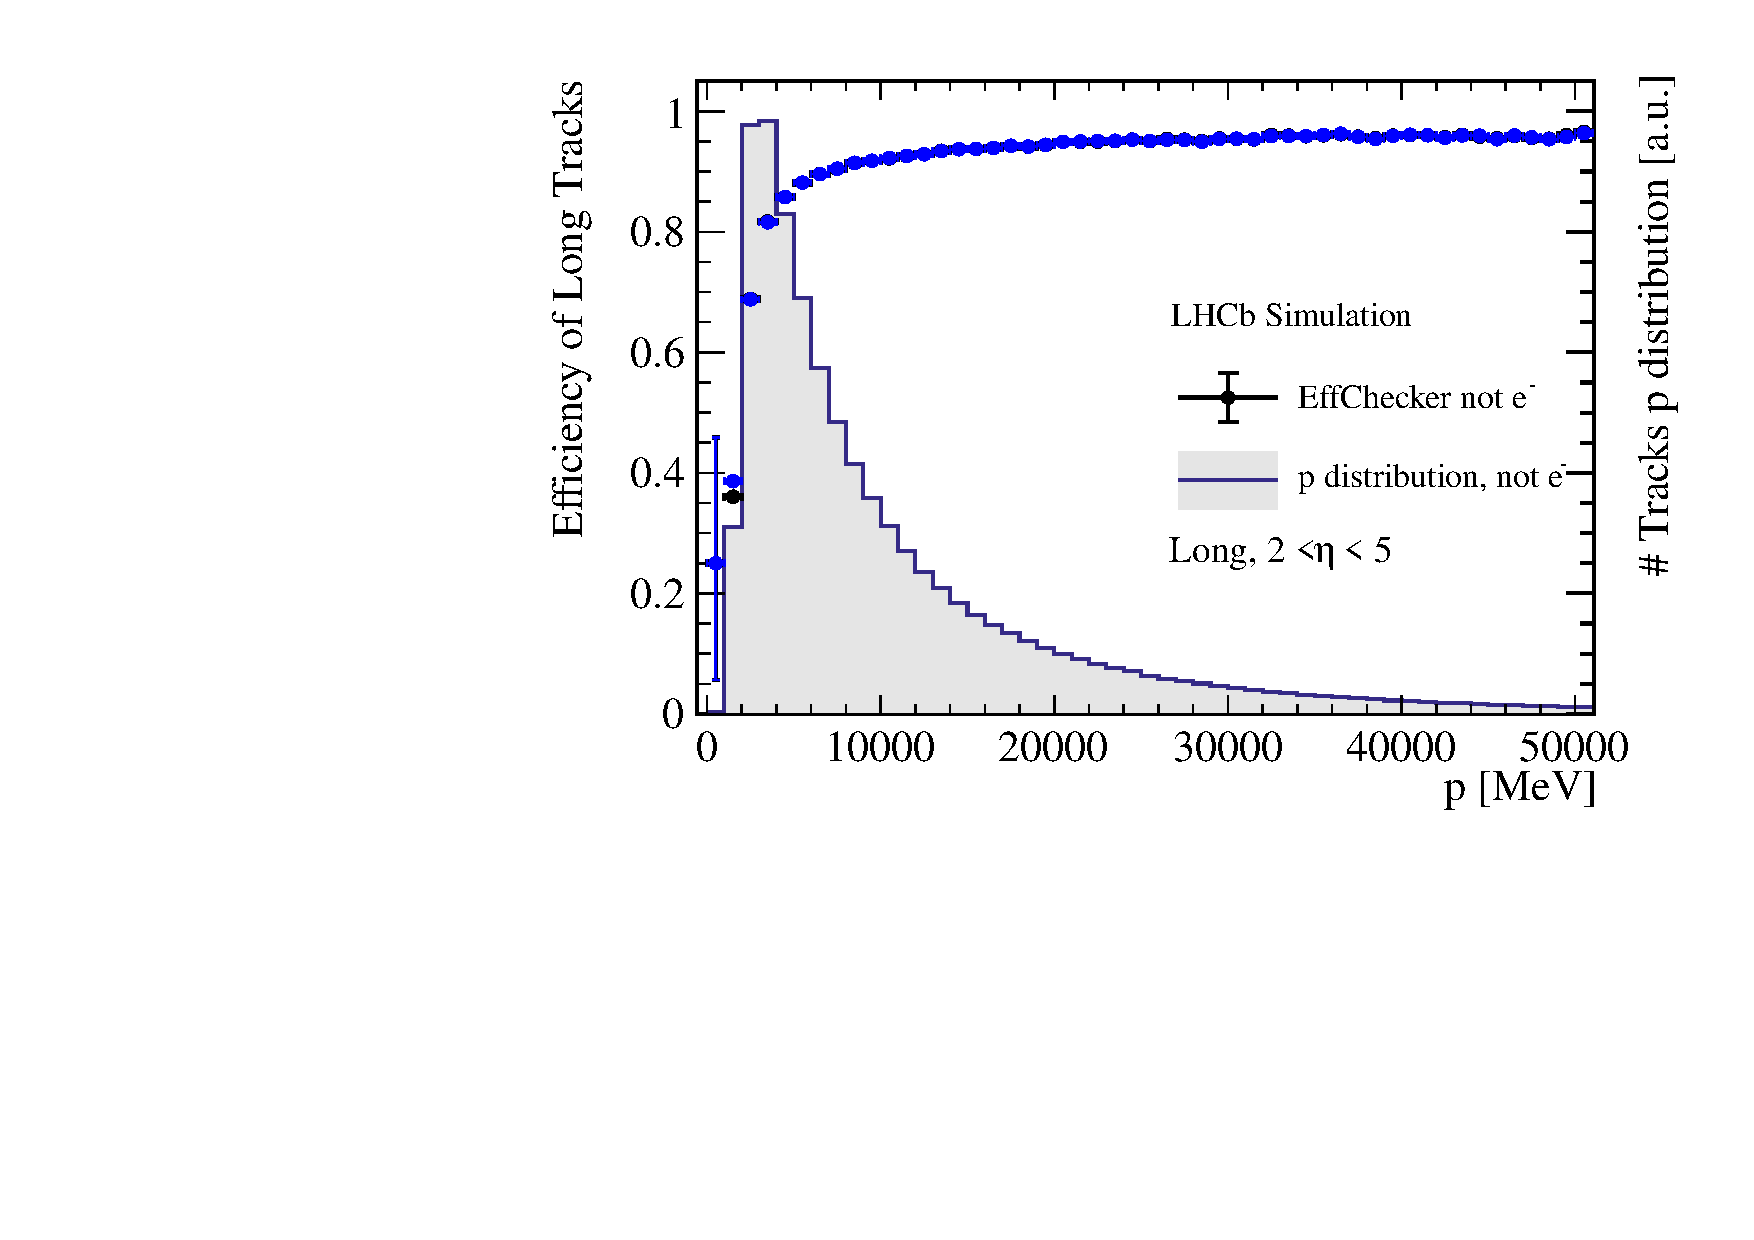
\includegraphics[width=1\textwidth]{Plots/TrackEfficiency_p_improved_MC_parameterisation.pdf}
    \end{subfigure}%
    \begin{subfigure}{0.45\textwidth}
      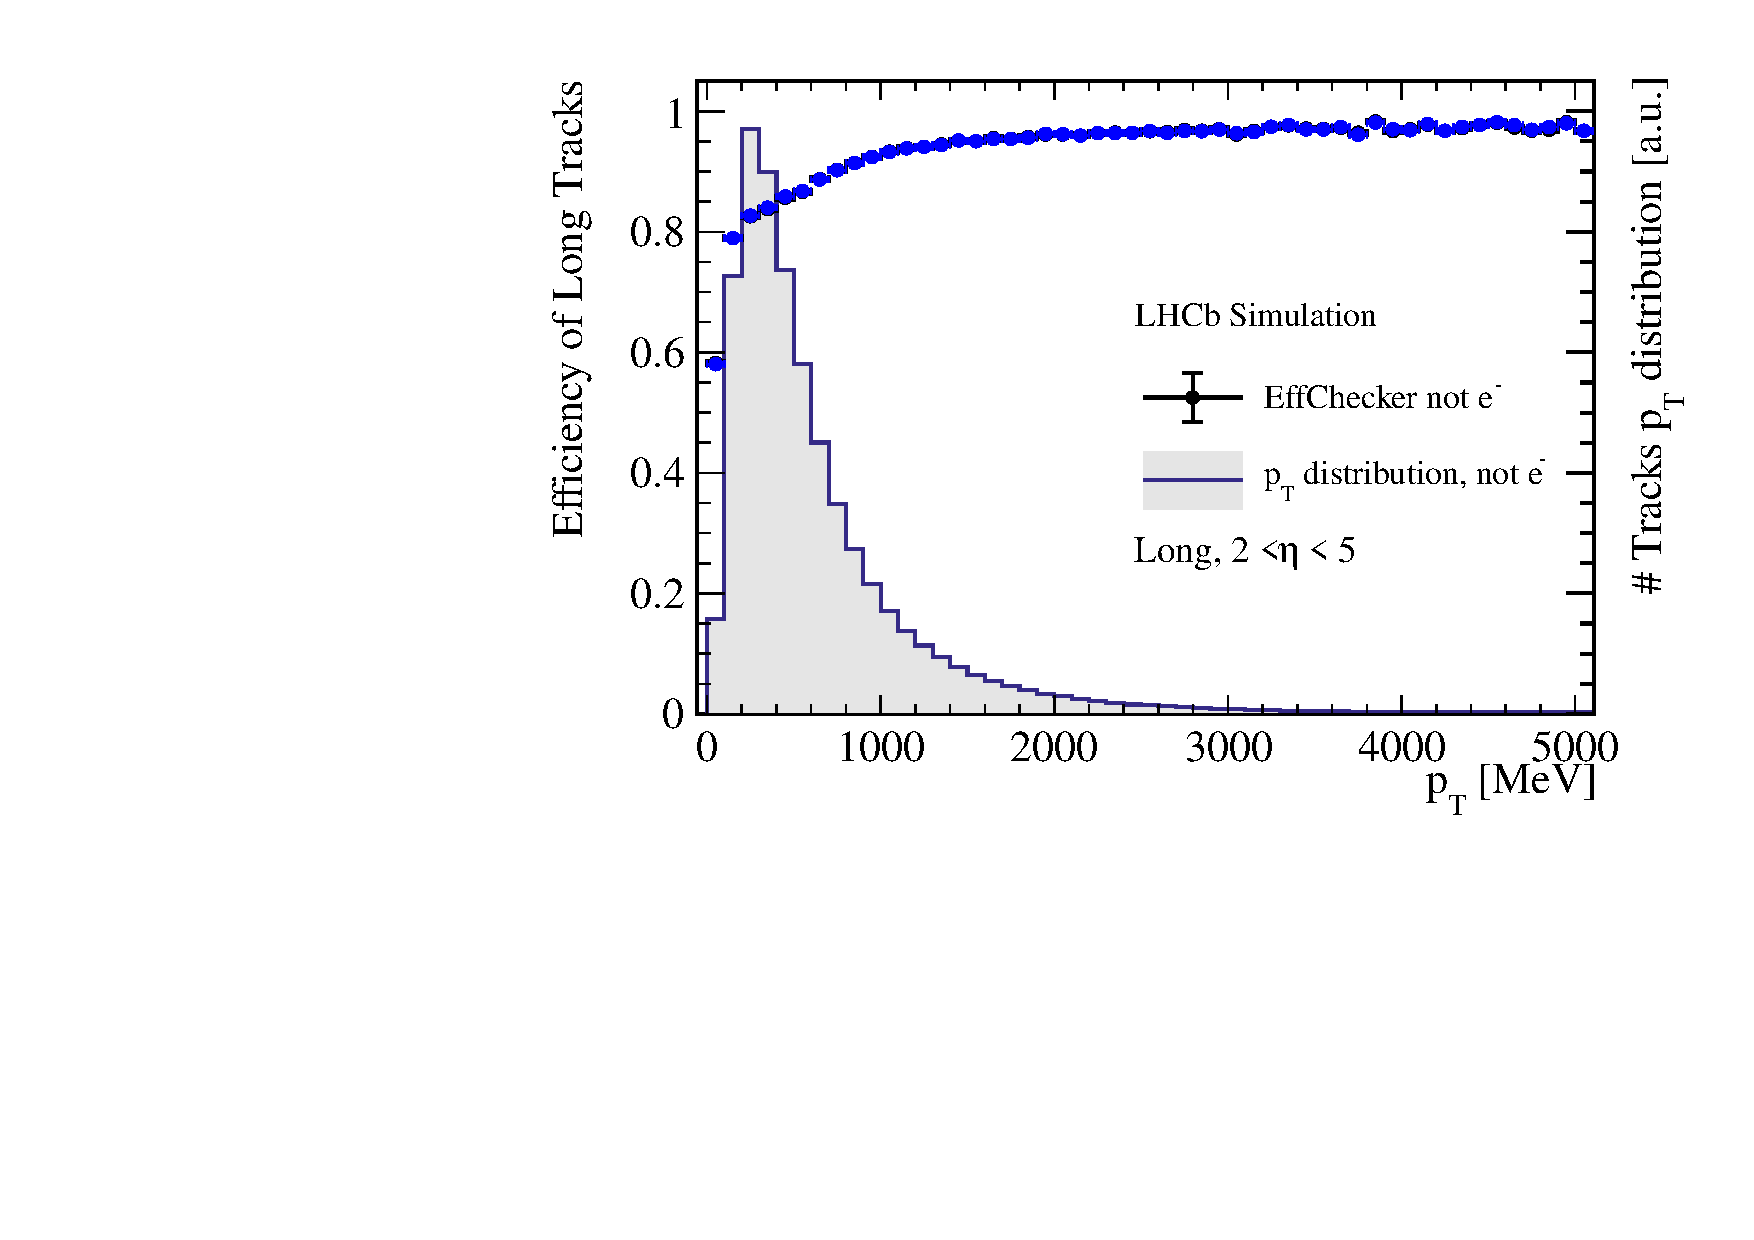
\includegraphics[width=1\textwidth]{Plots/TrackEfficiency_pt_improved_MC_parameterisation.pdf}
    \end{subfigure}
    \begin{subfigure}{0.45\textwidth}
      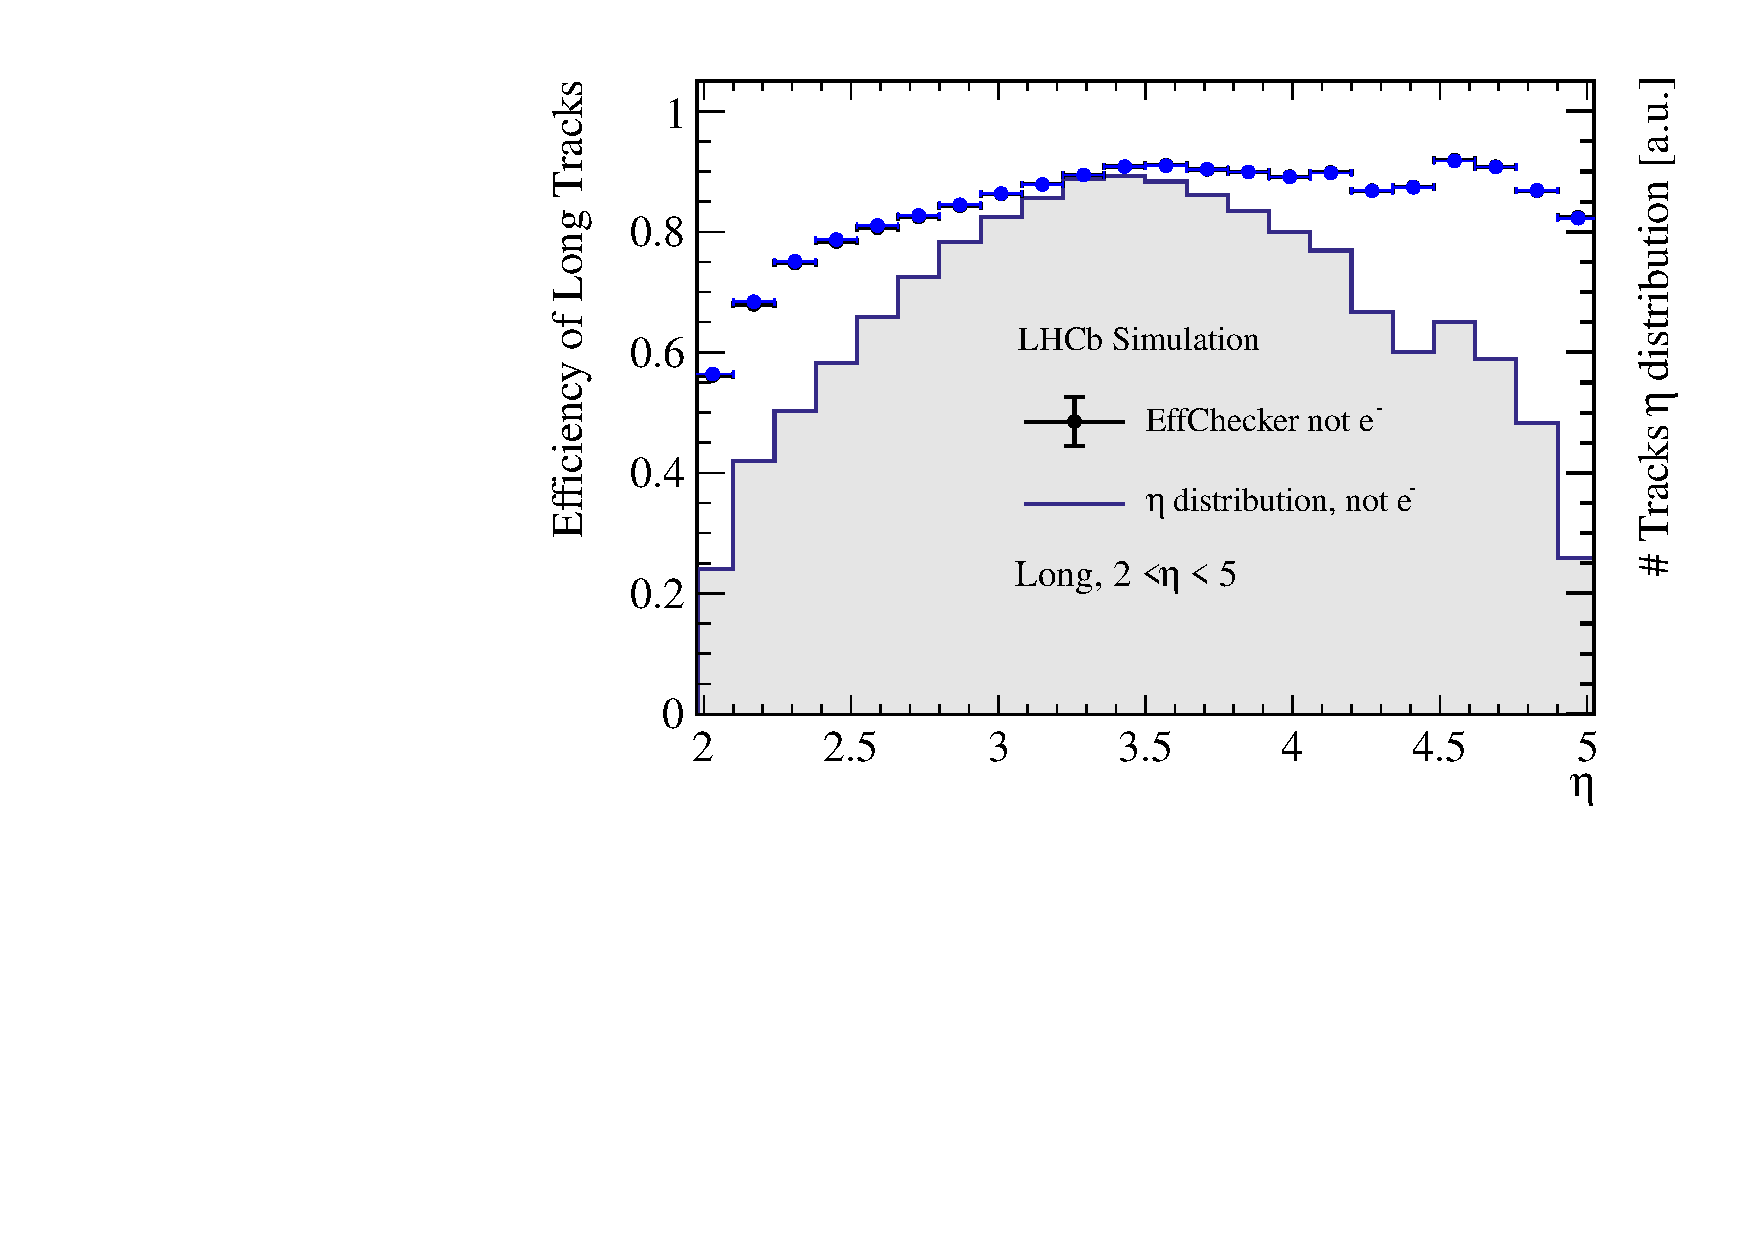
\includegraphics[width=1\textwidth]{Plots/TrackEfficiency_eta_improved_MC_parameterisation.pdf}
    \end{subfigure}%
    \begin{subfigure}{0.45\textwidth}
      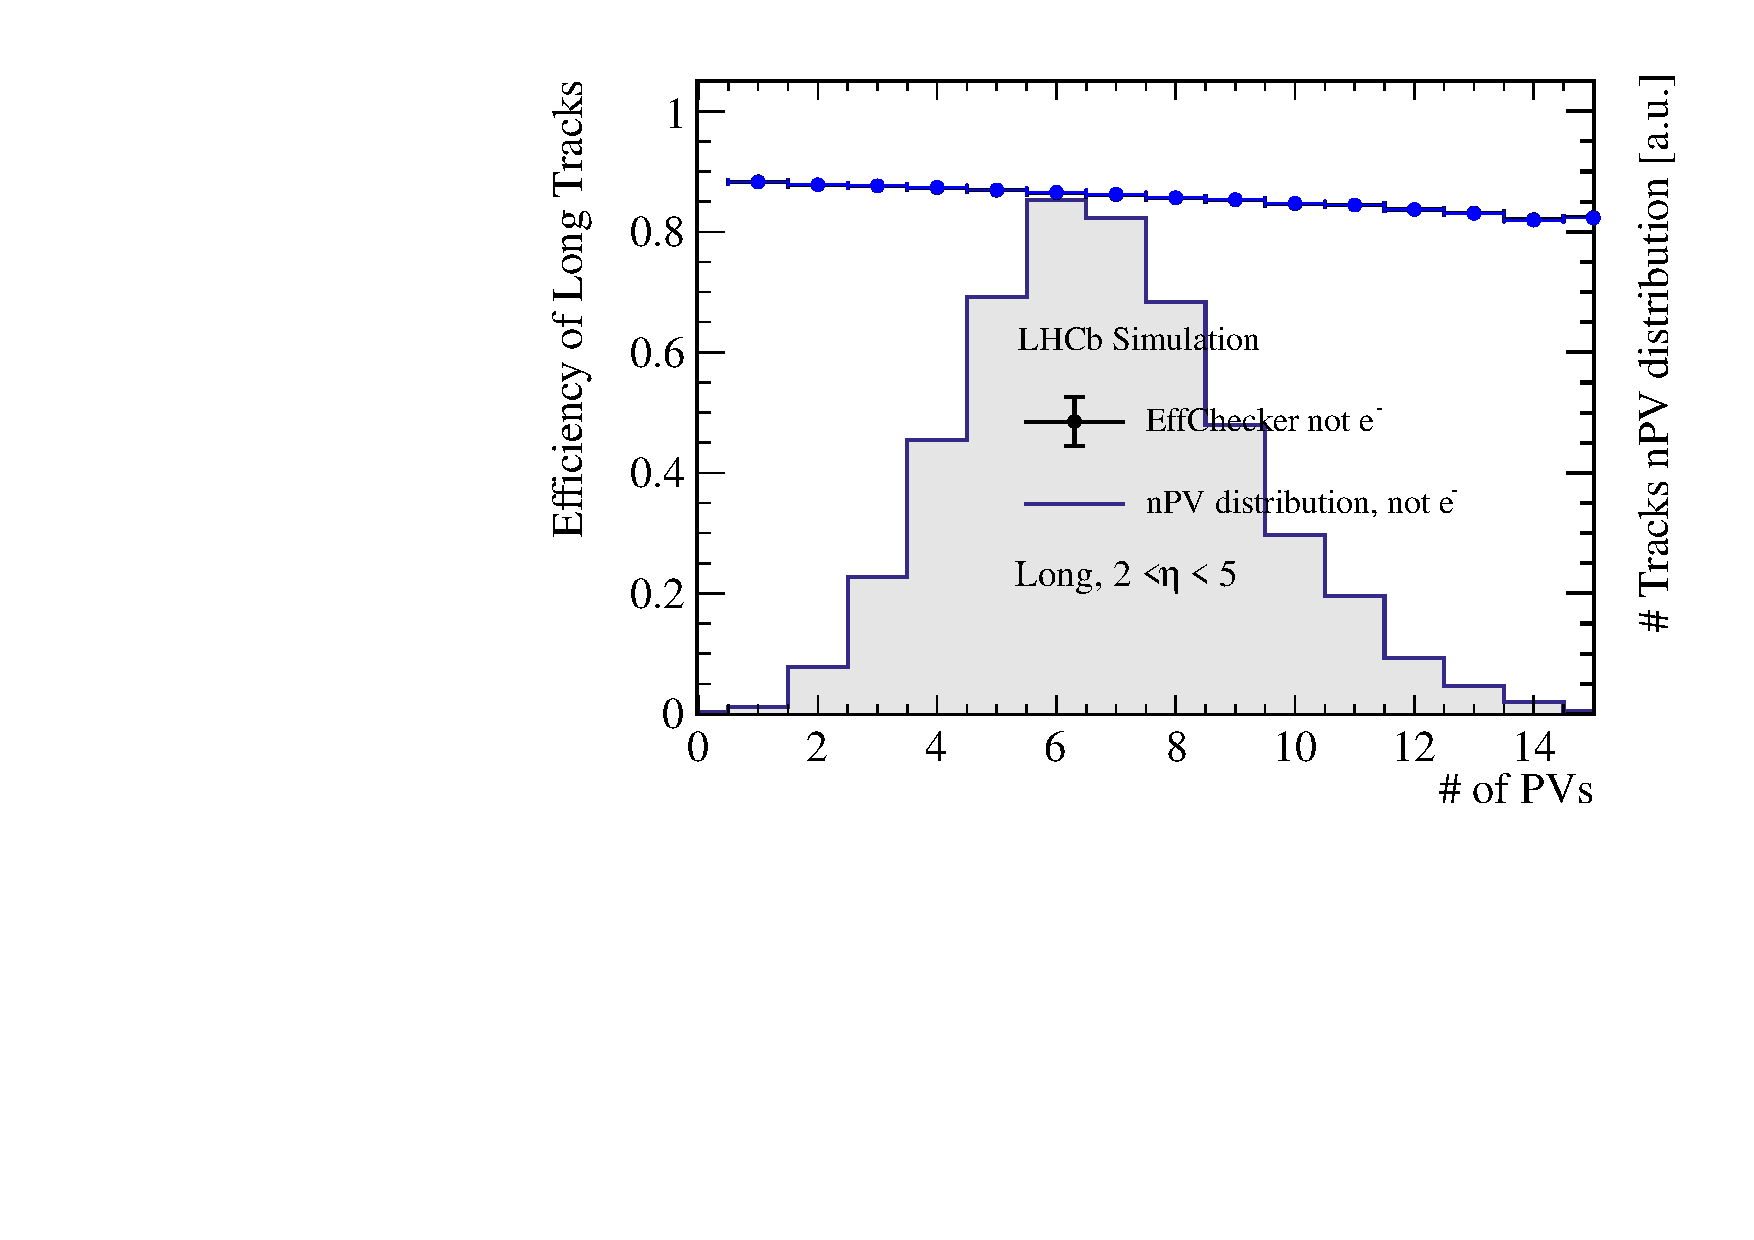
\includegraphics[width=1\textwidth]{Plots/TrackEfficiency_nPV_improved_MC_parameterisation.pdf}
    \end{subfigure}
    \vspace{-0.2cm}
    \caption*{Black: Old parameterisation. {\color{blue}Blue: Biased parameterisation of $z_{\rm mag}$} {\color{red}need to update these plots}.}
  \end{figure}
\end{frame}

\begin{frame}{Conclusion of $z_{\rm mag}$ studies}
  \vspace{0.0cm}
  \begin{itemize}
    \setlength\itemsep{1.0em}
    \item{Indeed, the improvement in performance when introducing a bias confirms that it is the search window size that drive the tracking efficiencies at low momentum}
    \item{Motivates us to keep the original $z_{\rm mag}$ parameterisation}
    \item{All other parameterisations will be updated using new MC samples}
    \item{I have already added these samples to TestDB in \href{https://gitlab.cern.ch/lhcb-datapkg/PRConfig/-/merge_requests/567}{this MR}}
    \item{I will also add documentation to the \href{https://gitlab.cern.ch/lhcb/paramscriptor}{ParamScriptor} repository}
  \end{itemize}
\end{frame}

\begin{frame}{Tracking efficiencies with final parameterisation}
  \vspace{0.0cm}
  \begin{figure}[htb]
    \centering
    \begin{subfigure}{0.45\textwidth}
      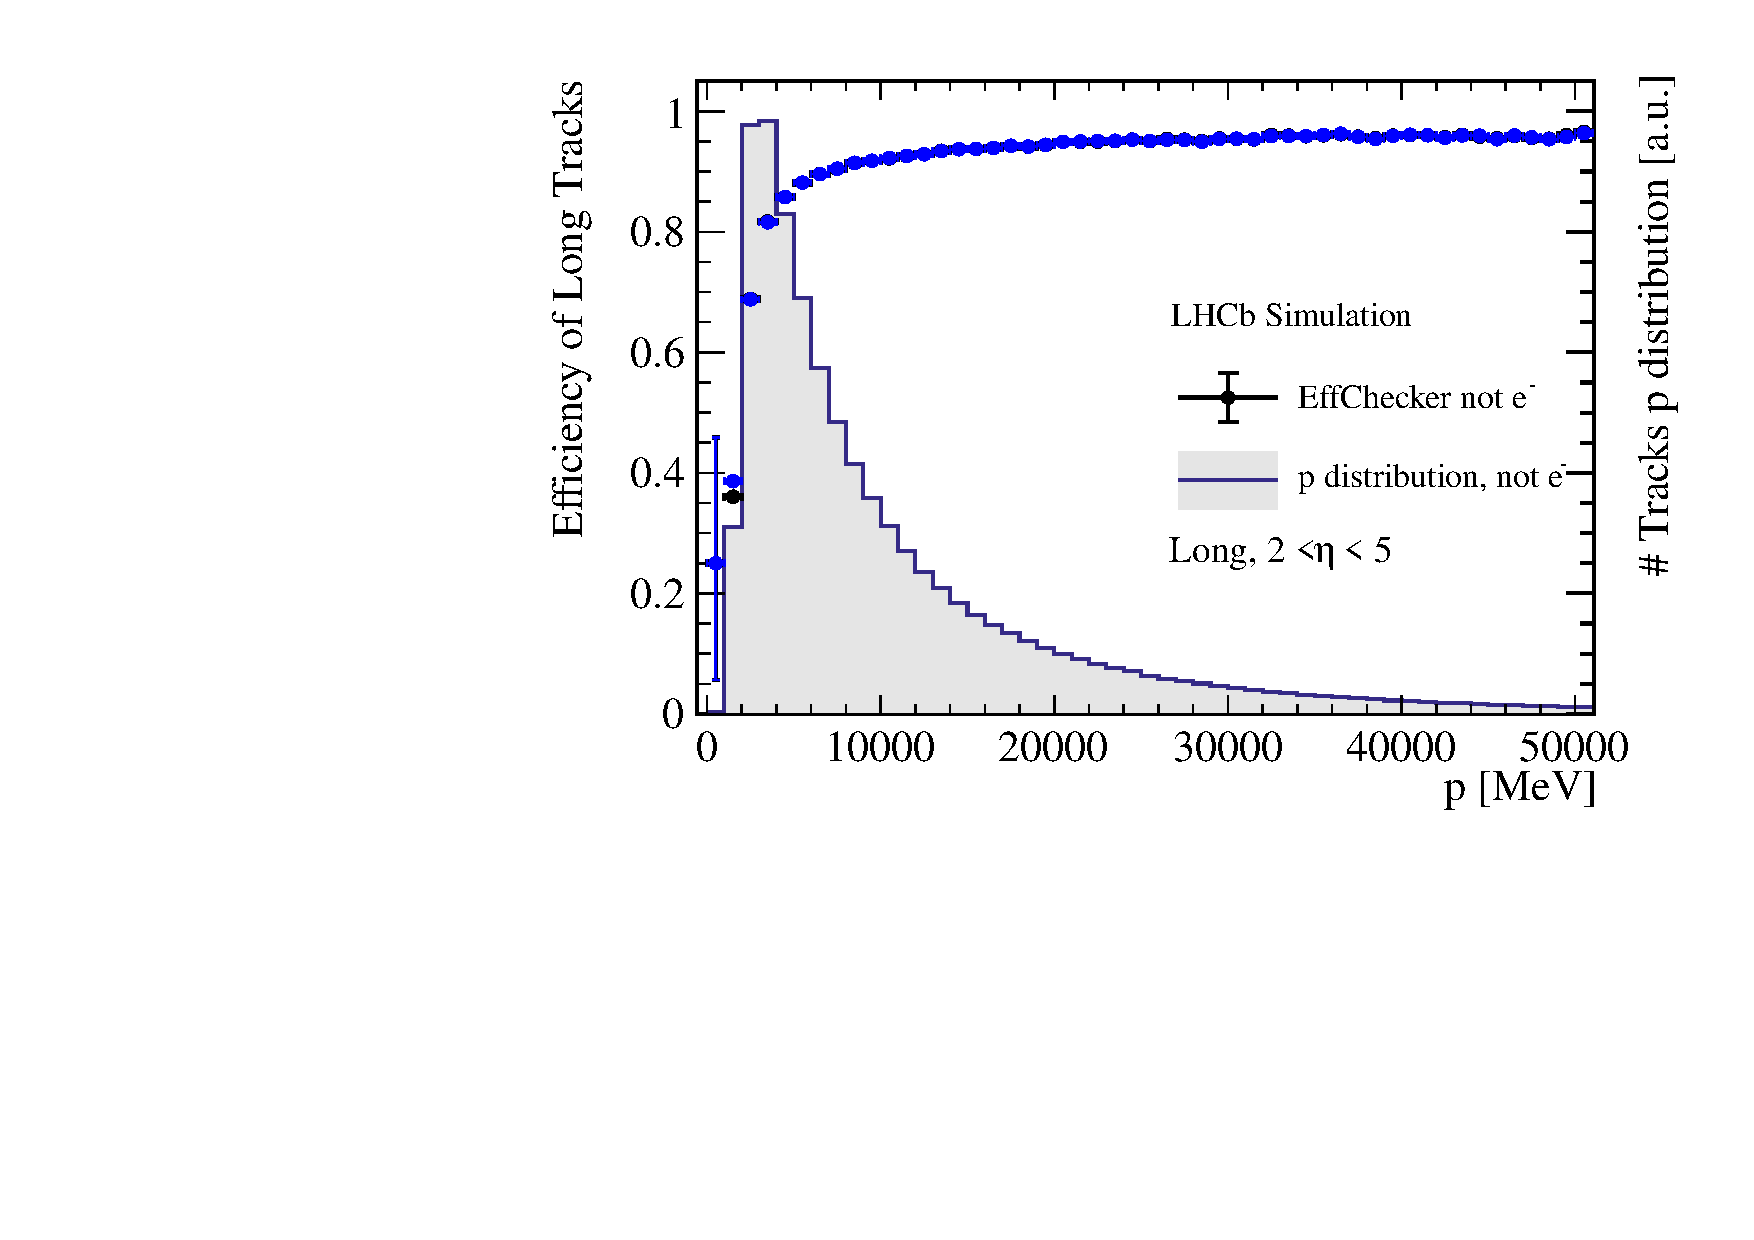
\includegraphics[width=1\textwidth]{Plots/TrackEfficiency_p_improved_MC_parameterisation.pdf}
    \end{subfigure}%
    \begin{subfigure}{0.45\textwidth}
      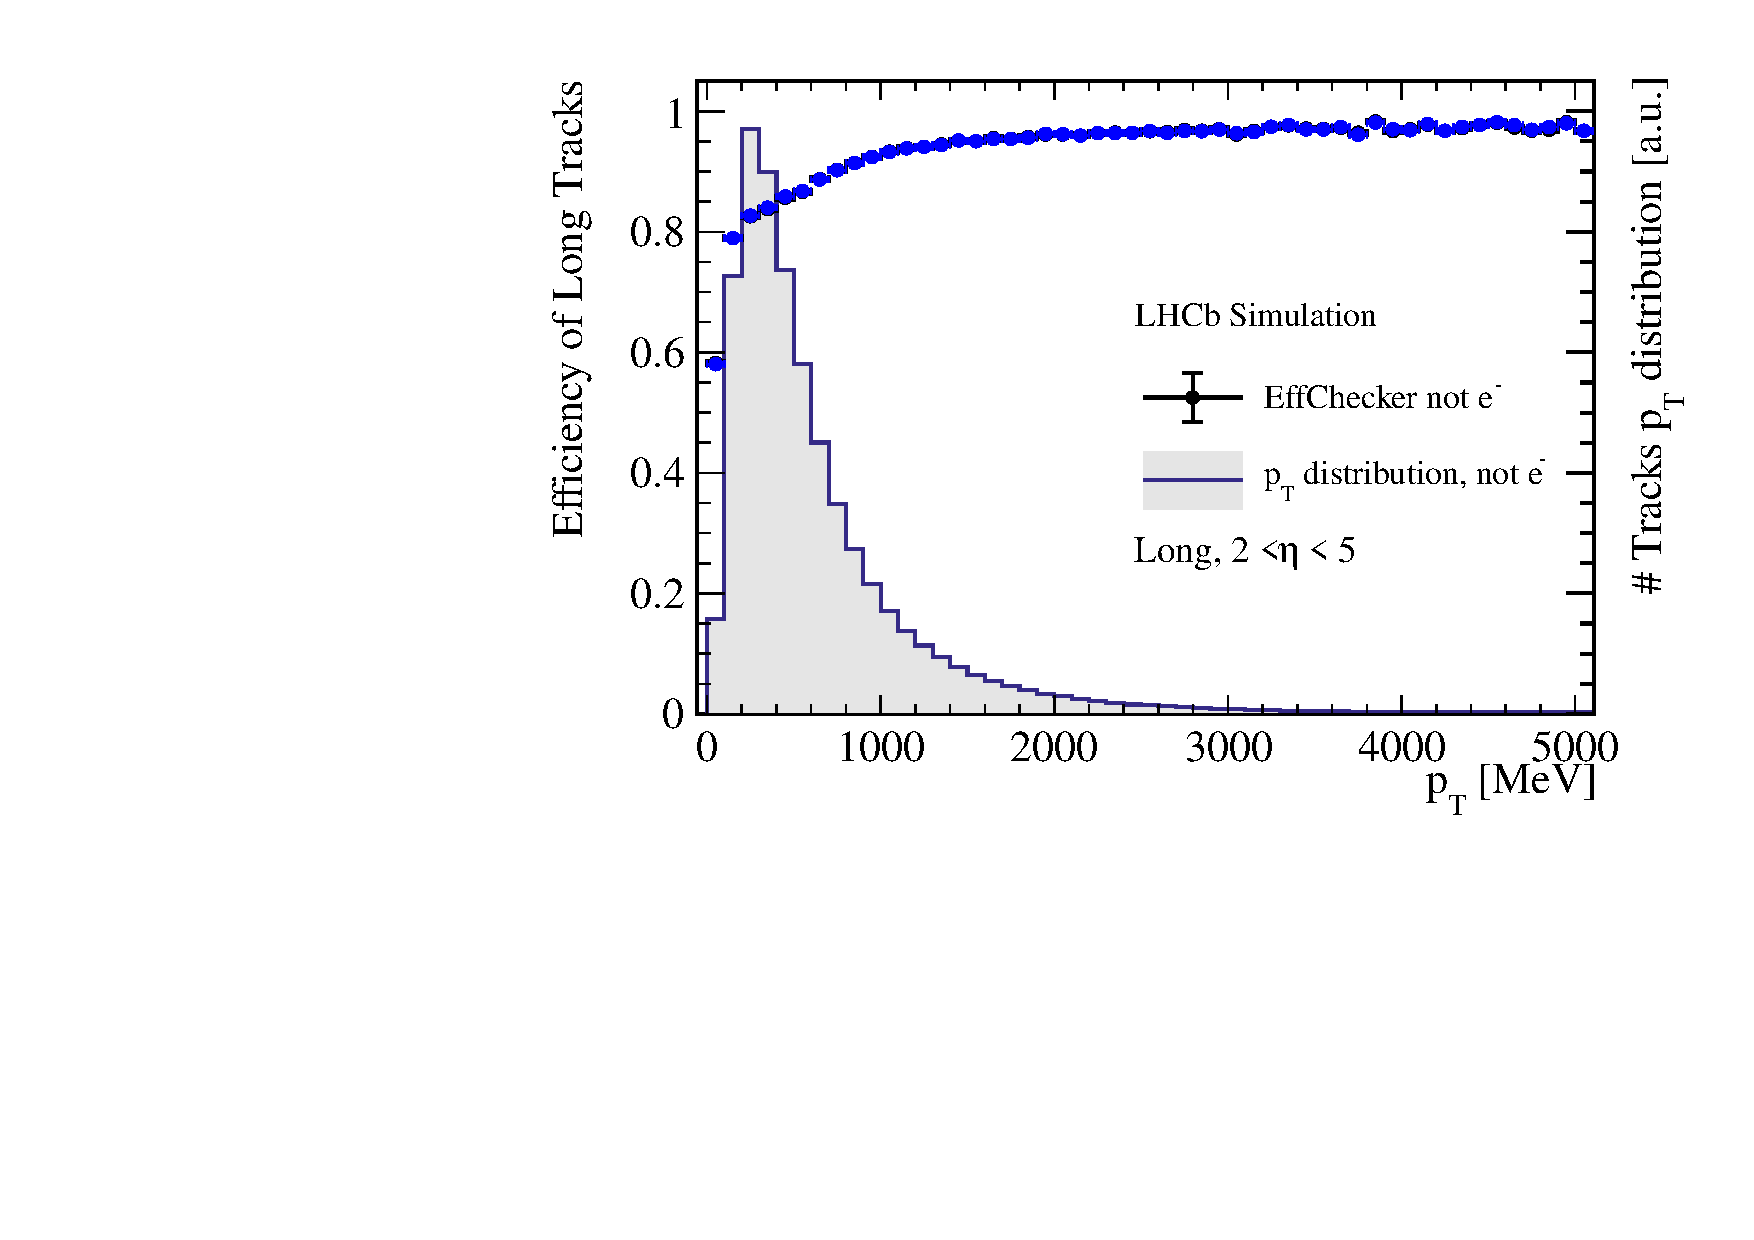
\includegraphics[width=1\textwidth]{Plots/TrackEfficiency_pt_improved_MC_parameterisation.pdf}
    \end{subfigure}
    \begin{subfigure}{0.45\textwidth}
      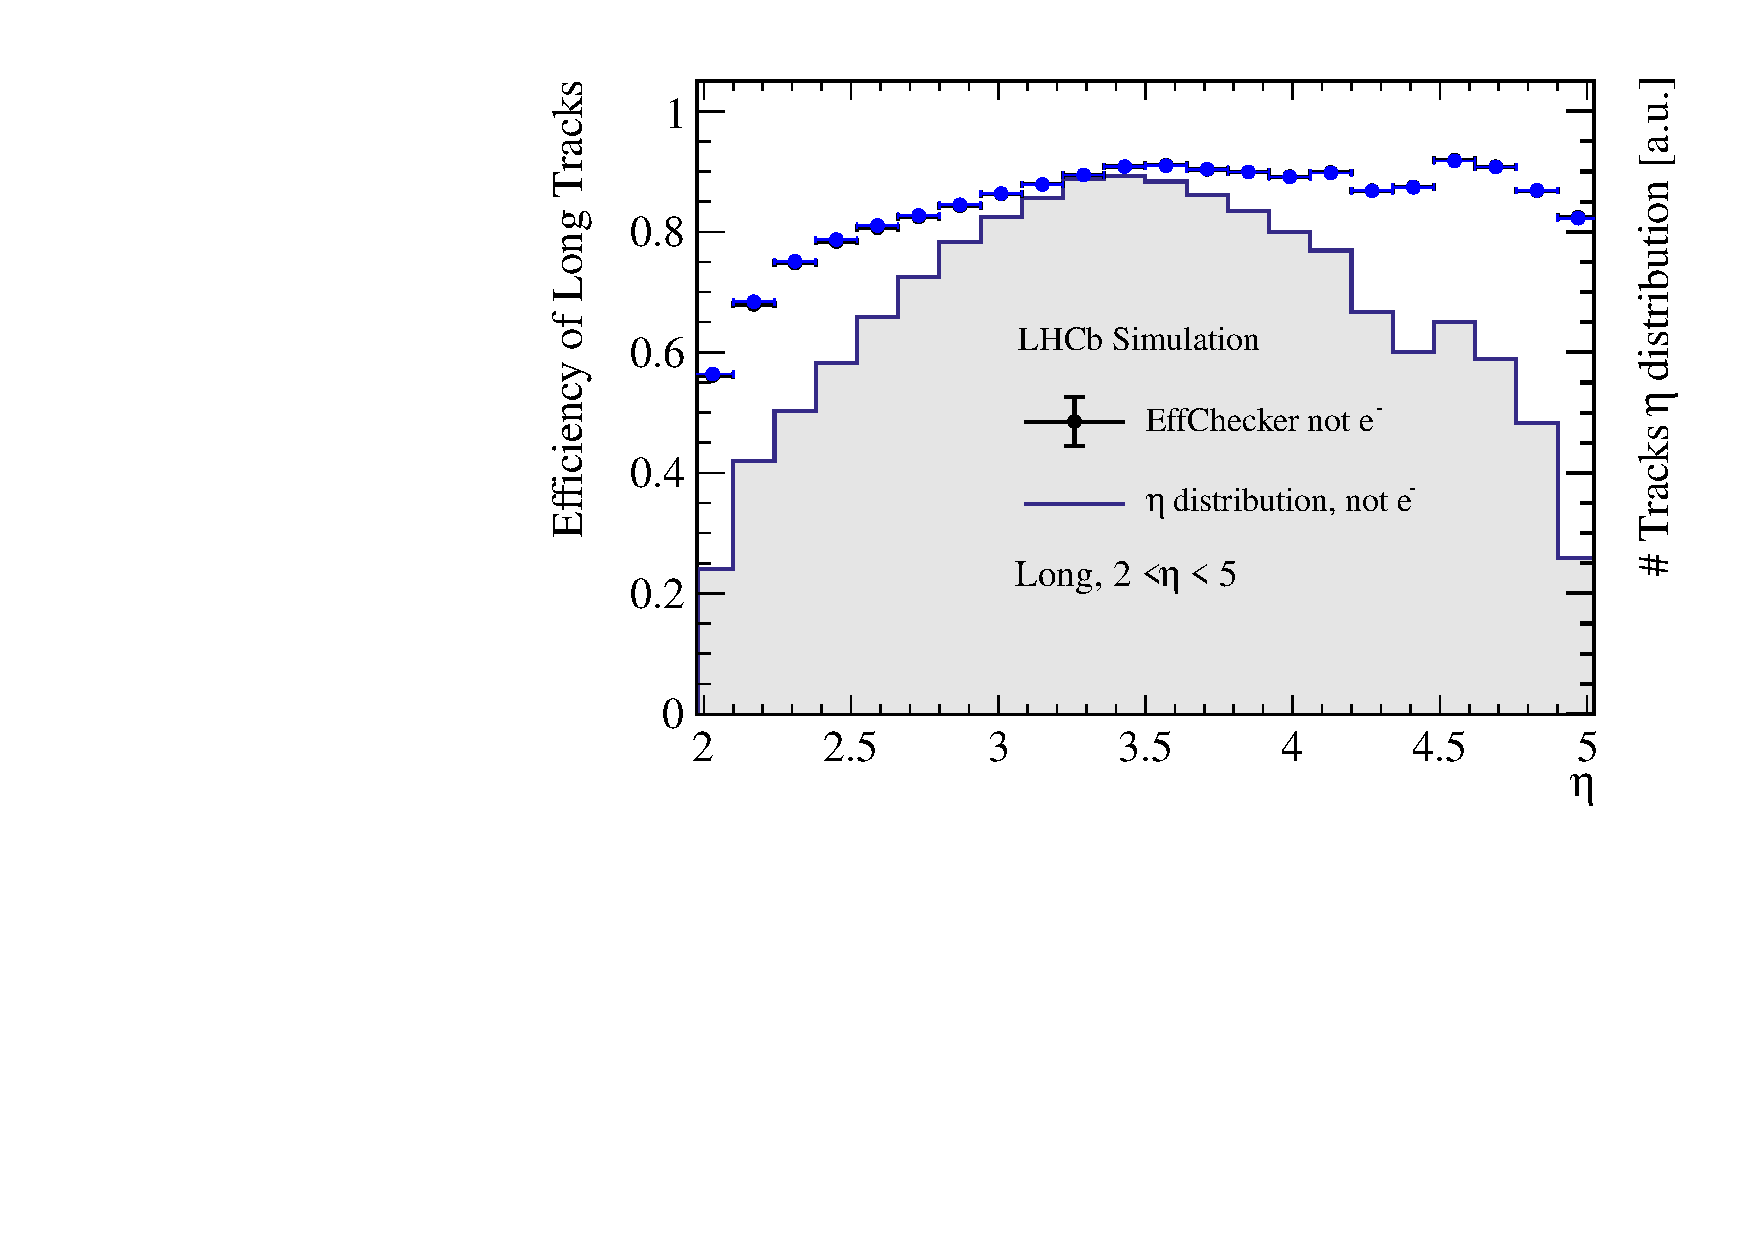
\includegraphics[width=1\textwidth]{Plots/TrackEfficiency_eta_improved_MC_parameterisation.pdf}
    \end{subfigure}%
    \begin{subfigure}{0.45\textwidth}
      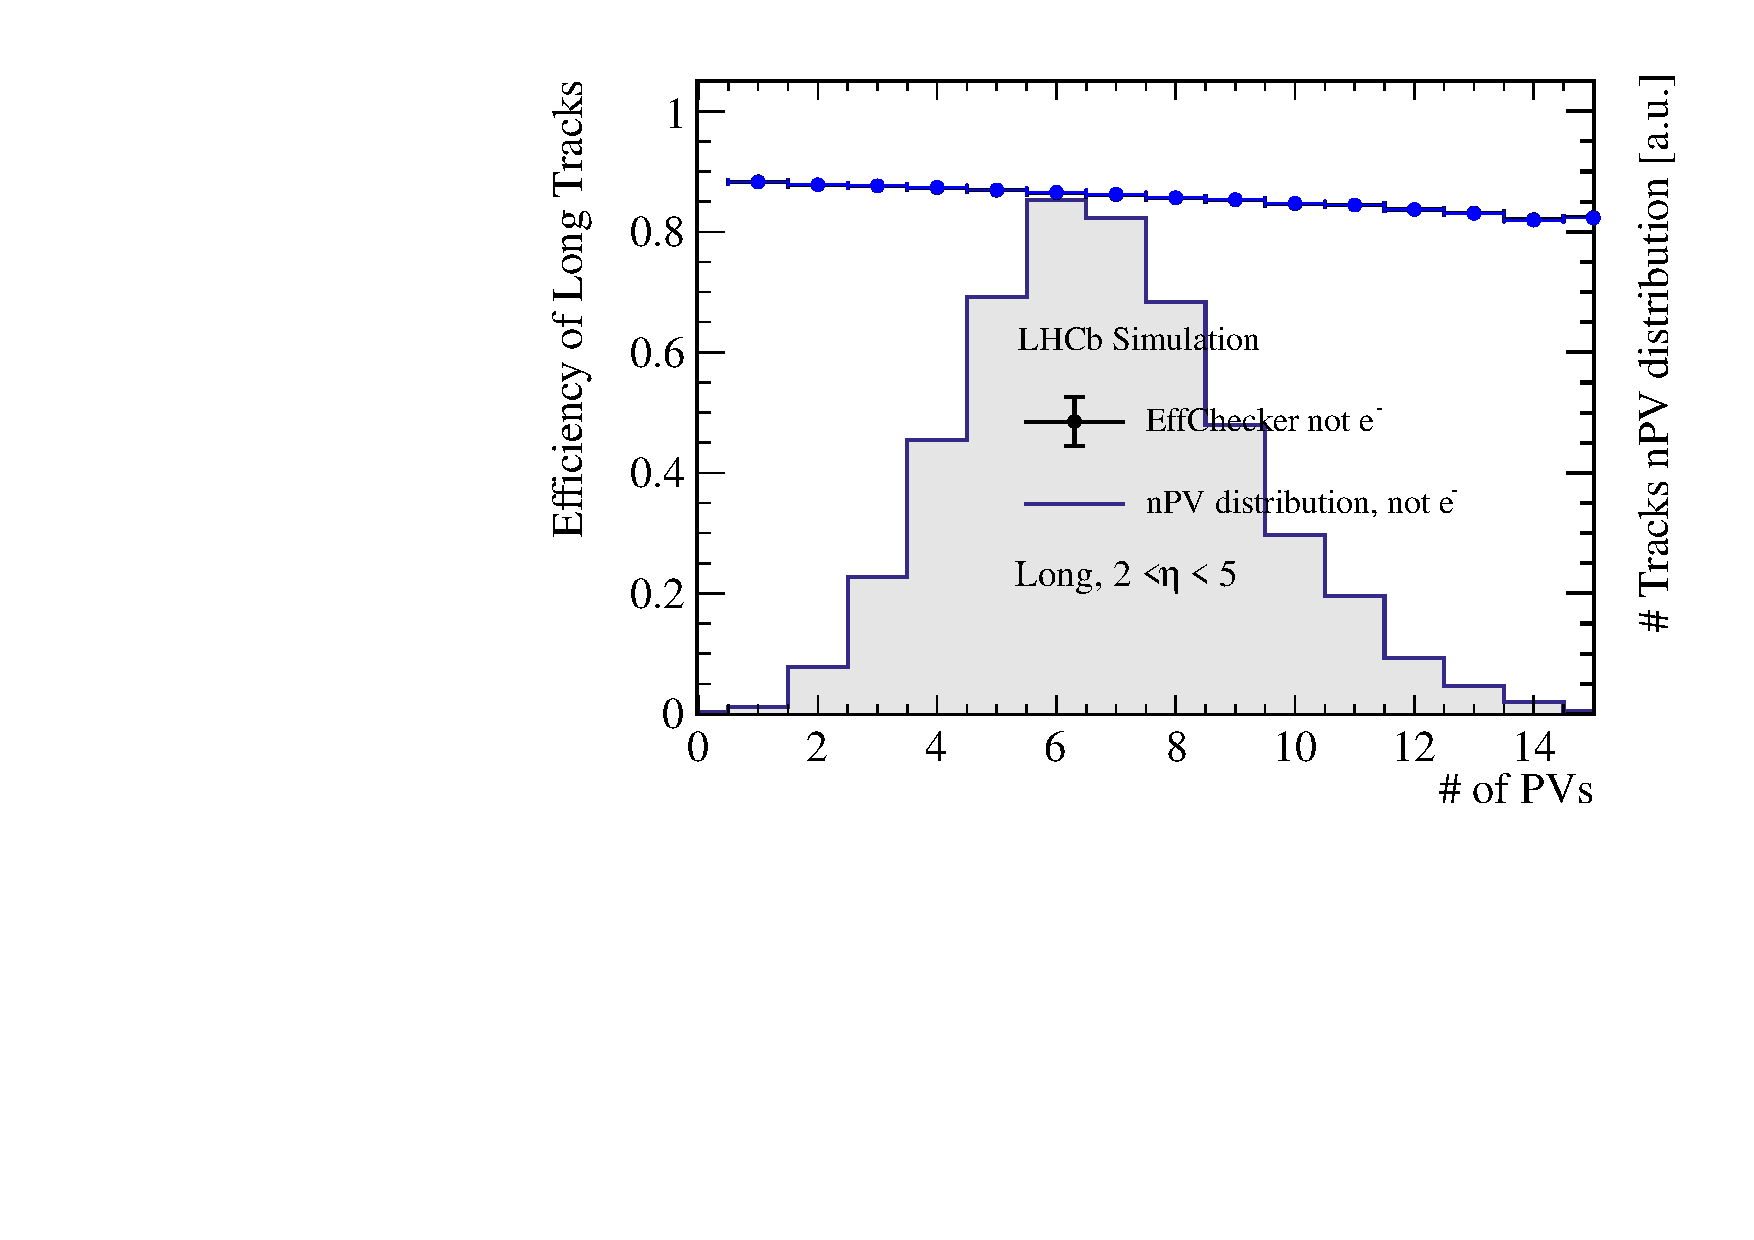
\includegraphics[width=1\textwidth]{Plots/TrackEfficiency_nPV_improved_MC_parameterisation.pdf}
    \end{subfigure}
    \vspace{-0.2cm}
    \caption*{Black: Old parameterisation. {\color{blue}Blue: Proposed parameterisation} {\color{red}need to update these plots}.}
  \end{figure}
\end{frame}

\begin{frame}{Momentum resolution with final parameterisation}
  \vspace{0.0cm}
  \begin{figure}[htb]
    \centering
    \begin{subfigure}{0.50\textwidth}
      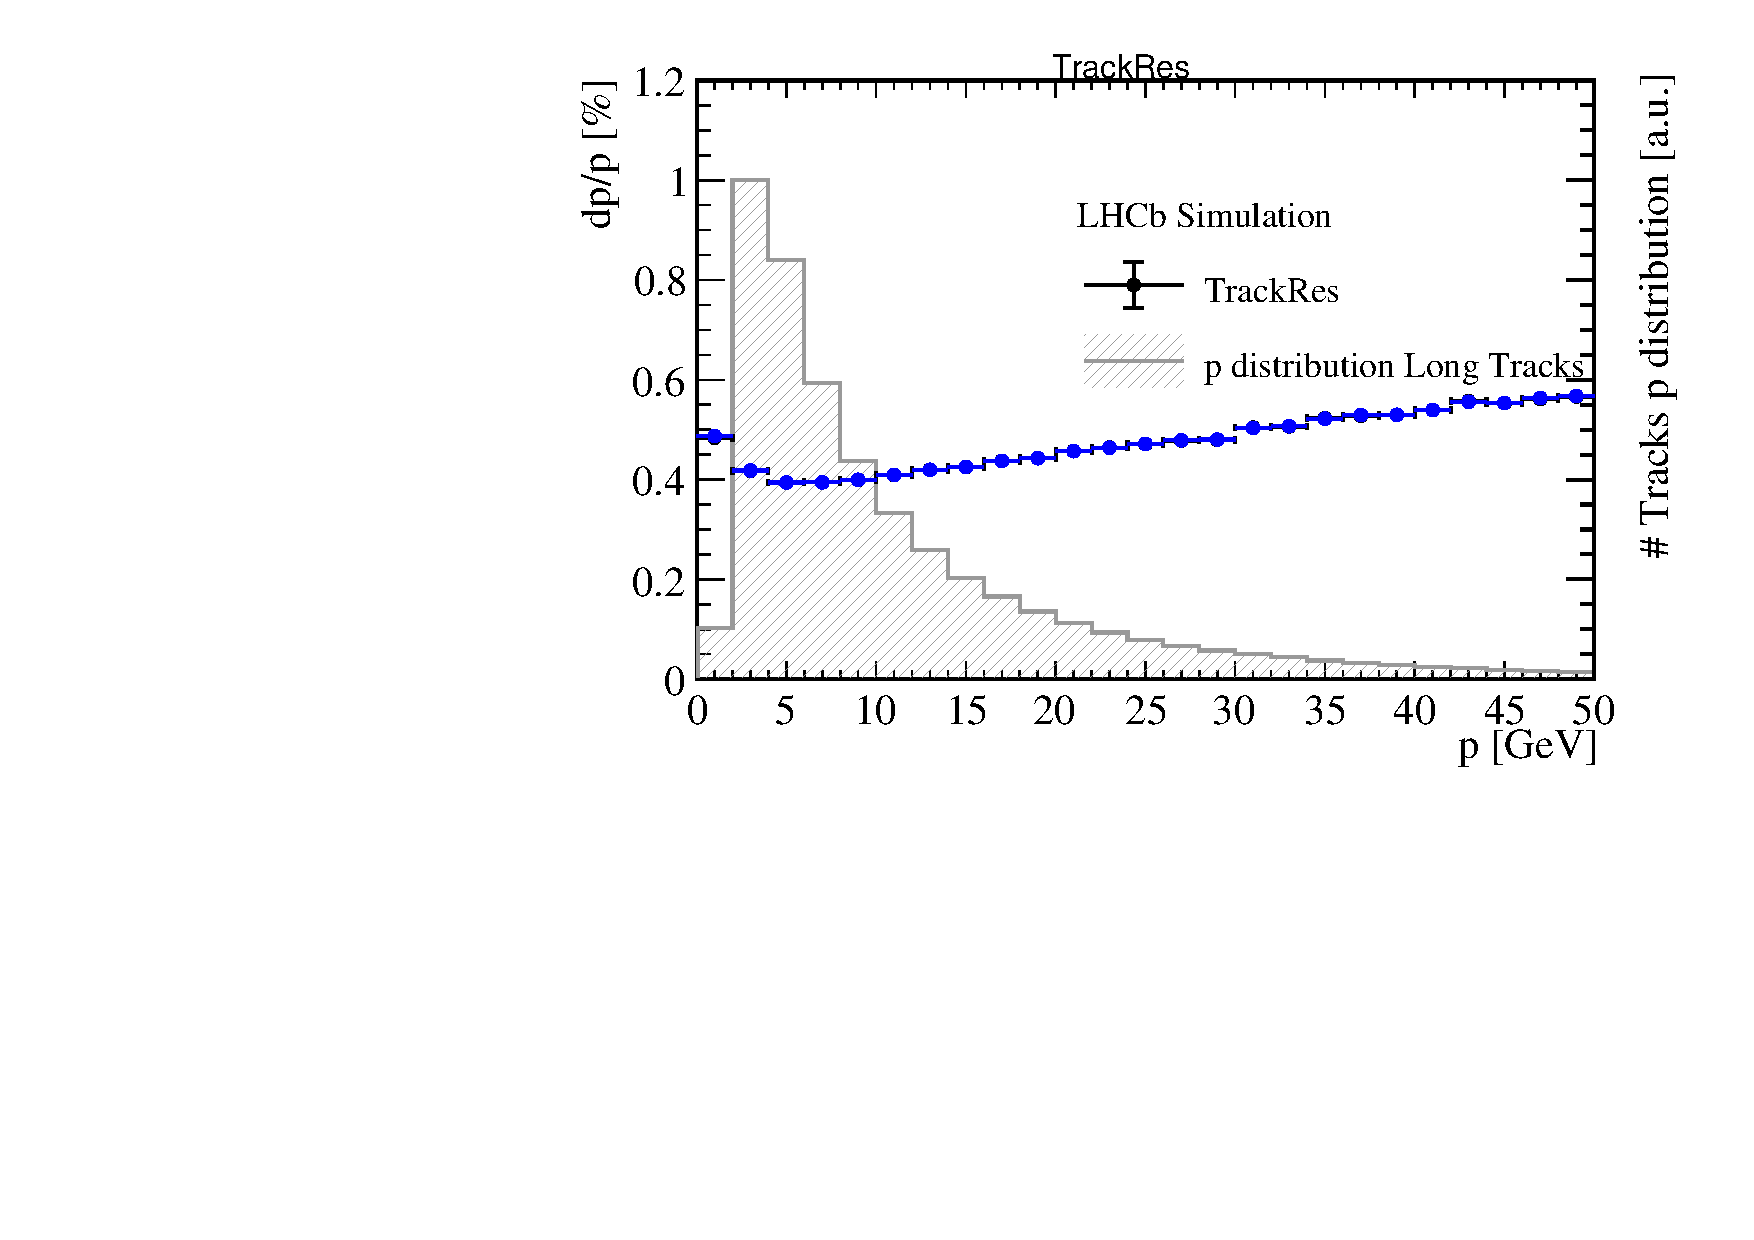
\includegraphics[width=1\textwidth]{Plots/Track_resolution_p_comparison.pdf}
    \end{subfigure}%
    \begin{subfigure}{0.50\textwidth}
      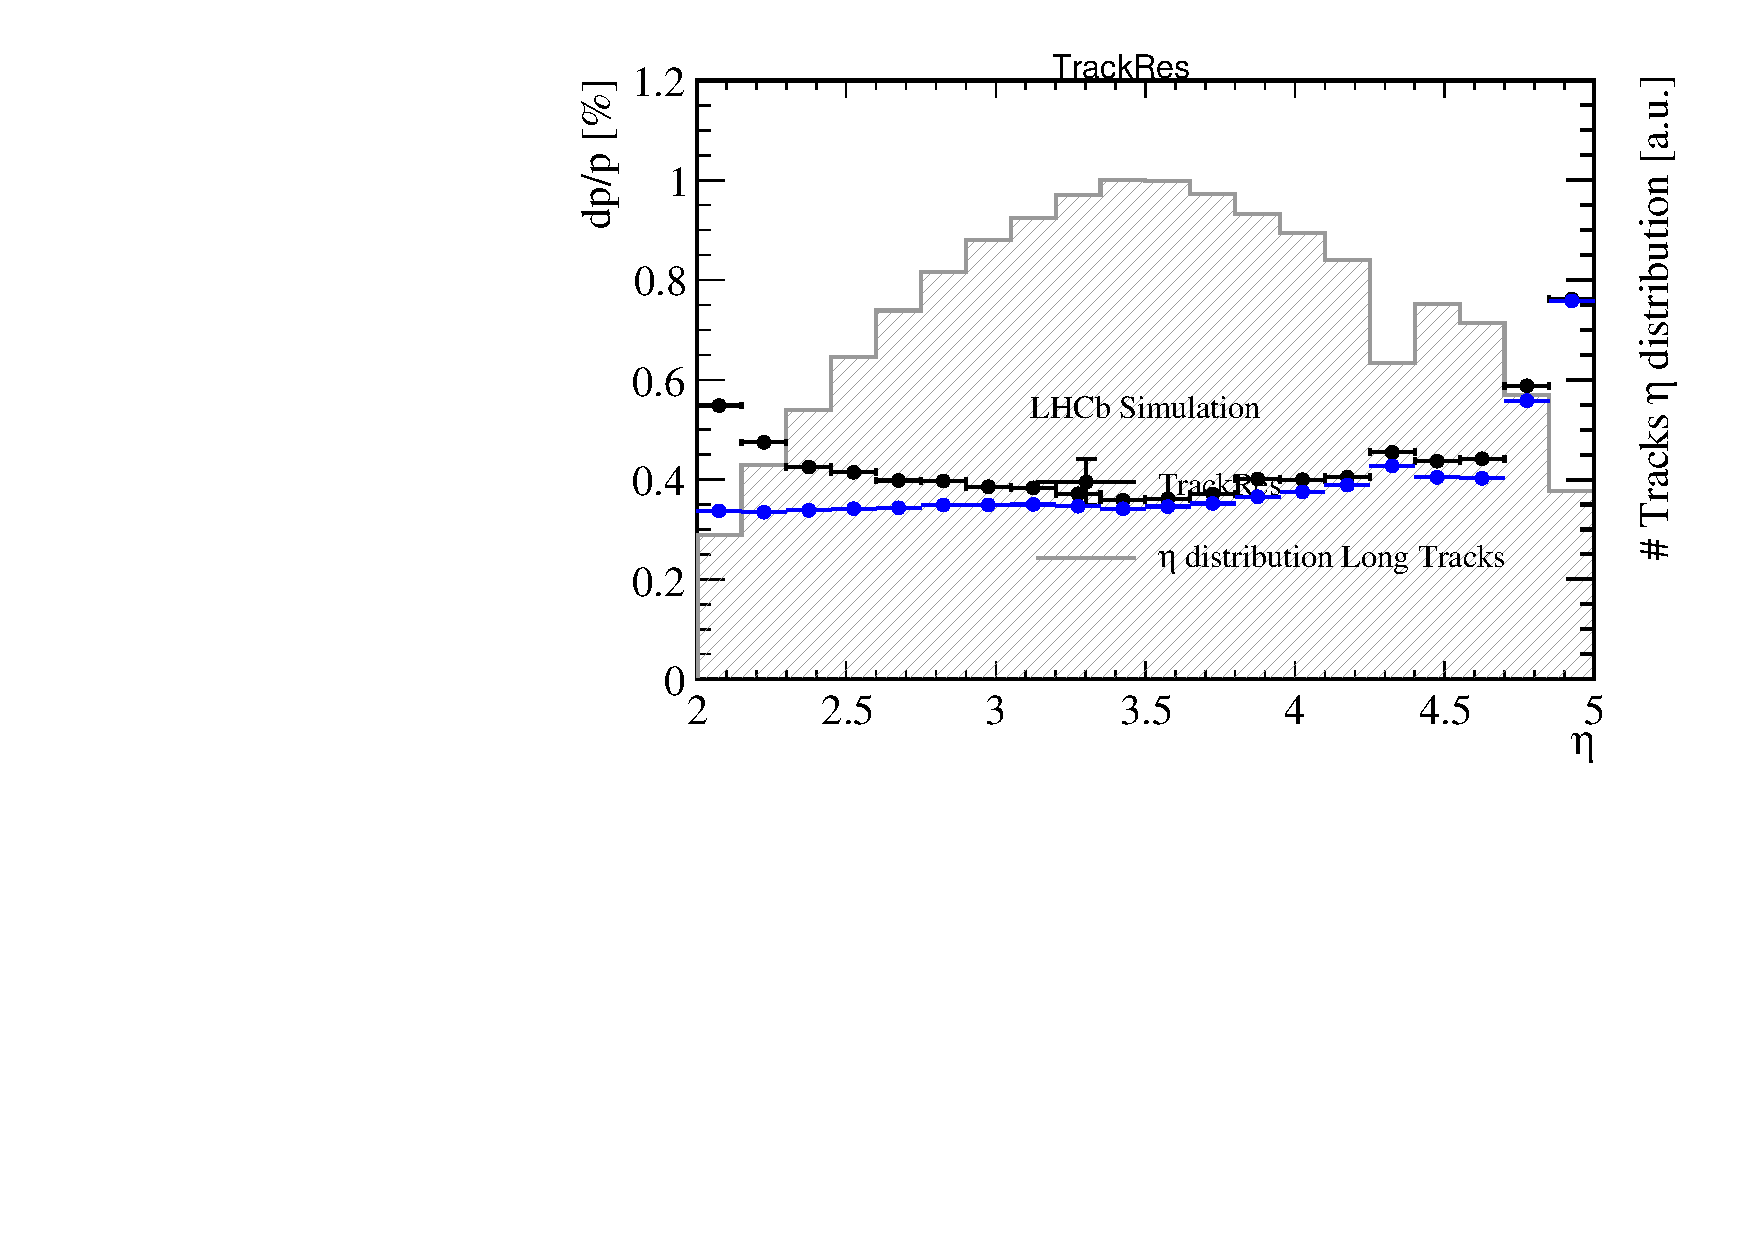
\includegraphics[width=1\textwidth]{Plots/Track_resolution_eta_comparison.pdf}
    \end{subfigure}
    \vspace{-0.2cm}
    \caption*{Black: Old parameterisation. {\color{blue}Blue: Proposed parameterisation}. {\color{red}need to update these plots}}
  \end{figure}
\end{frame}

\section{Conclusion}

\begin{frame}{Summary}
  \vspace{0.0cm}
  \begin{itemize}
    \setlength\itemsep{1.0em}
    \item{All parameterisations have been updated using centrally produced MC}
    \begin{enumerate}
      \item{Larger MC samples}
      \item{Both magnet polarities}
      \item{Larger selection of decay modes}
    \end{enumerate}
    \item{Possible improvements to $z_{\rm mag}$ parameterisation have been explored}
    \begin{itemize}
      \setlength\itemsep{0.3em}
      \item{Biases are reduced, but performance gets \underline{worse}}
      \item{Reason for this unexpected behaviour:}
      \begin{itemize}
        \item[-]{Original parameterisation mostly \underline{underestimated} $z_{\rm mag}$}
        \item[$\to$]{\underline{Overestimated} search windows in the $x$-plane}
        \item[$\to$]{More hits included in reconstruction}
        \item[$\to$]{Higher tracking reconstruction}
      \end{itemize}
    \end{itemize}
    \item{I propose: Update all parameterisations except for that of $z_{\rm mag}$}
    \begin{itemize}
      \item[-]{Negligible change in tracking efficiencies}
      \item[-]{Small improvement in momentum resolution}
    \end{itemize}
  \end{itemize}
\end{frame}

\begin{frame}{Next steps}
  \vspace{0.0cm}
  \begin{enumerate}
    \setlength\itemsep{2.0em}
    \item{Get \href{https://gitlab.cern.ch/lhcb/Rec/-/merge_requests/4362}{!4362} and \href{https://gitlab.cern.ch/lhcb-datapkg/PRConfig/-/merge_requests/567}{!567} merged}
    \item{Document work in ParamScriptor}
    \item{Final step: Improve throughput}
    \begin{itemize}
      \item{Code was already heavily optimised by Andre G{\"u}nther...}
      \item{...but I'll do some quick checks for obvious bottleknecks}
    \end{itemize}
  \end{enumerate}
  \vspace{0.3cm}
  \begin{center}
    \Huge Thanks for listening!
  \end{center}
\end{frame}

\end{document}
